%--------------------------------------------%
% Template Beamer para Apresentações da UFRN %
% by alcemygvseverino@gmail.com              %
% Baseado em MIT Beamer Template			 %
% versao 1.1								 %
% Atualizado em 14/05/2016					 %
%--------------------------------------------%
\documentclass[handout,t]{beamer}
% Para alterar a linguagem do documento
\usepackage[portuges]{babel}
% Para aceitar caracteres especias deretamente do teclado
\usepackage[utf8]{inputenc}
% Para seguir as normas da ABNT de citacao e referencias
\usepackage[alf]{abntex2cite}
% Para incluir figuras
\usepackage{graphicx}
% Para melhor ajuste da posisao das figuras
\usepackage{float}
% Para ajustar as dimensoes do layout da pagina
\usepackage{geometry}
% Para formatar estrutura e informacoes de formulas matematicas
\usepackage{amsmath}
% Para incluir simbolos especiais em formulas matematicas
\usepackage{amssymb}
% Para incluir links nas referencias
\usepackage{url}
% Para incluir paginas de documentos .pdf externos
\usepackage{pgfpages}
% Para ajustar o estilo dos contadores
\usepackage{enumerate}
% Para modificar a cor do texto
\usepackage{color}
% Para incluir condicoes
\usepackage{ifthen}
% Para colocar legendas em algo que nao e float
\usepackage{capt-of}
% Para definir o tema do slide
\usetheme{Berlin}
% Para difinir cores e background
\usecolortheme{ufrn}
% Para numerar as figuras
\setbeamertemplate{caption}[numbered]

% Pacotes adicionais
\usepackage{xcolor}
%\usepackage{listings}
\usepackage[utf8]{inputenc}
%\usepackage[framed,numbered,autolinebreaks,useliterate]{mcode}
\usepackage{subfig}
\usepackage{minted}


% Título
\title[Projeto por discretização de filtros contínuos]{
	Projeto de Filtro IIR}
% Data
\date{
	\today}
% Autores
\author[Lenival Gomes]{
	Lenival Gomes% \inst{1}\\
	%\vspace{0.25cm}
	%Autor 02 \inst{2}
	}
% Instituto
\institute[INSTITUTO]{
	%\inst{1}%
	\url{lenival@ufrn.edu.br}\\
	\vspace{0.25cm}
	%\inst{2}%
	Pós-Graduação em Engenharia Mecatrônica\\
	Universidade Federal do Rio Grande do Norte}
% Logo do canto inferior direito
%\pgfdeclareimage[height=0.8cm]{logo_ufrn}{figuras/logo_ufrn}
\pgfdeclareimage[height=0.8cm]{logo_lapps}{figuras/logo_lapps}
%\pgfdeclareimage[height=0.8cm]{logo_shell}{figuras/Shell-logo}
\pgfdeclareimage[height=0.8cm]{logo_npit}{figuras/logo_npit}
\pgfdeclareimage[height=0.8cm]{logo_imd}{figuras/logo_imd}
\logo{
	\vspace*{-0.15cm}
	%\pgfuseimage{logo_ufrn}
	\pgfuseimage{logo_lapps}
	%\pgfuseimage{logo_shell}
    \pgfuseimage{logo_npit}
    \pgfuseimage{logo_imd}
	\hspace*{-0.05cm}
    }


\begin{document}
% Sumário
\frame{\titlepage}
\section[]{}
\begin{frame}{Sumário}
	\tableofcontents
\end{frame}


\AtBeginSection[]
{
\begin{frame}
\frametitle{Resumo}
\tableofcontents[currentsection]
\end{frame}
}


% Introducao
\section{Introdução}
\begin{frame}{Introdução}
\begin{itemize}
    \item Um sinal de áudio corrompido por ruído colorido será gerado
	\item Serão projetados filtros IIR que removam este ruído
	\item Os filtros serão projetados e testado no MATLAB
	\item O processo de desenvolvimento será detalhado
	\item Gráficos com os resultados serão gerados
	\item A análise dos resultados será feita através dos gráficos 
\end{itemize}
	
\end{frame}

% Metodologia
\section{Metodologia}


\begin{frame}{Visão Geral}
    \begin{itemize}
        \item Obtêm-se sinal de áudio
        \item Inicializa-se parâmetros do sinal, ruído e filtros
        \item Gera-se ruído colorido e adiciona-se ao áudio
        \item Projeta-se filtros a partir do visto em \cite{oppenheim2013discrete} e \cite{chaparro2010signals}
        \begin{itemize}
            \item Define-se Ordem
            \item Calcula-se coeficientes
            \item Discretiza-se sistema obtido
        \end{itemize}
        \item Filtra-se sinal degradado pelo ruído
        \item Gera-se gráficos
        \item Reproduz-se áudio filtrado

    \end{itemize}
\end{frame}



% As built
\section{Como Construído}

\begin{frame}{Preparação do sinal de áudio corrompido}
	O sinal de áudio conterá:
	\begin{itemize}
	    \item Voz;
	    \item Ruído Branco limitado à faixa de 300 Hz em trono de 2 kHz
	\end{itemize}
	    \begin{figure}[!htb]
        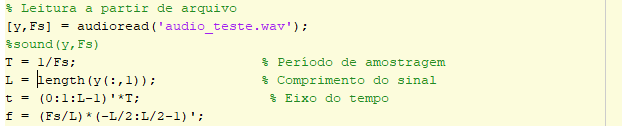
\includegraphics[width=0.7\textwidth]{graficos/code_audio.png}
        \end{figure} 
    	\begin{figure}[!htb]
        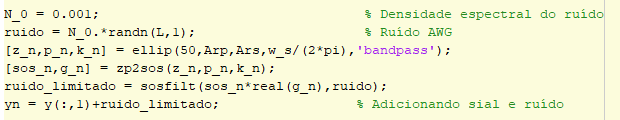
\includegraphics[width=0.7\textwidth]{graficos/code_ruido.png}
        \end{figure} 

\end{frame}

\begin{frame}{Áudio original}
    \begin{figure}[!htb]
        \centering
        \subfloat{
        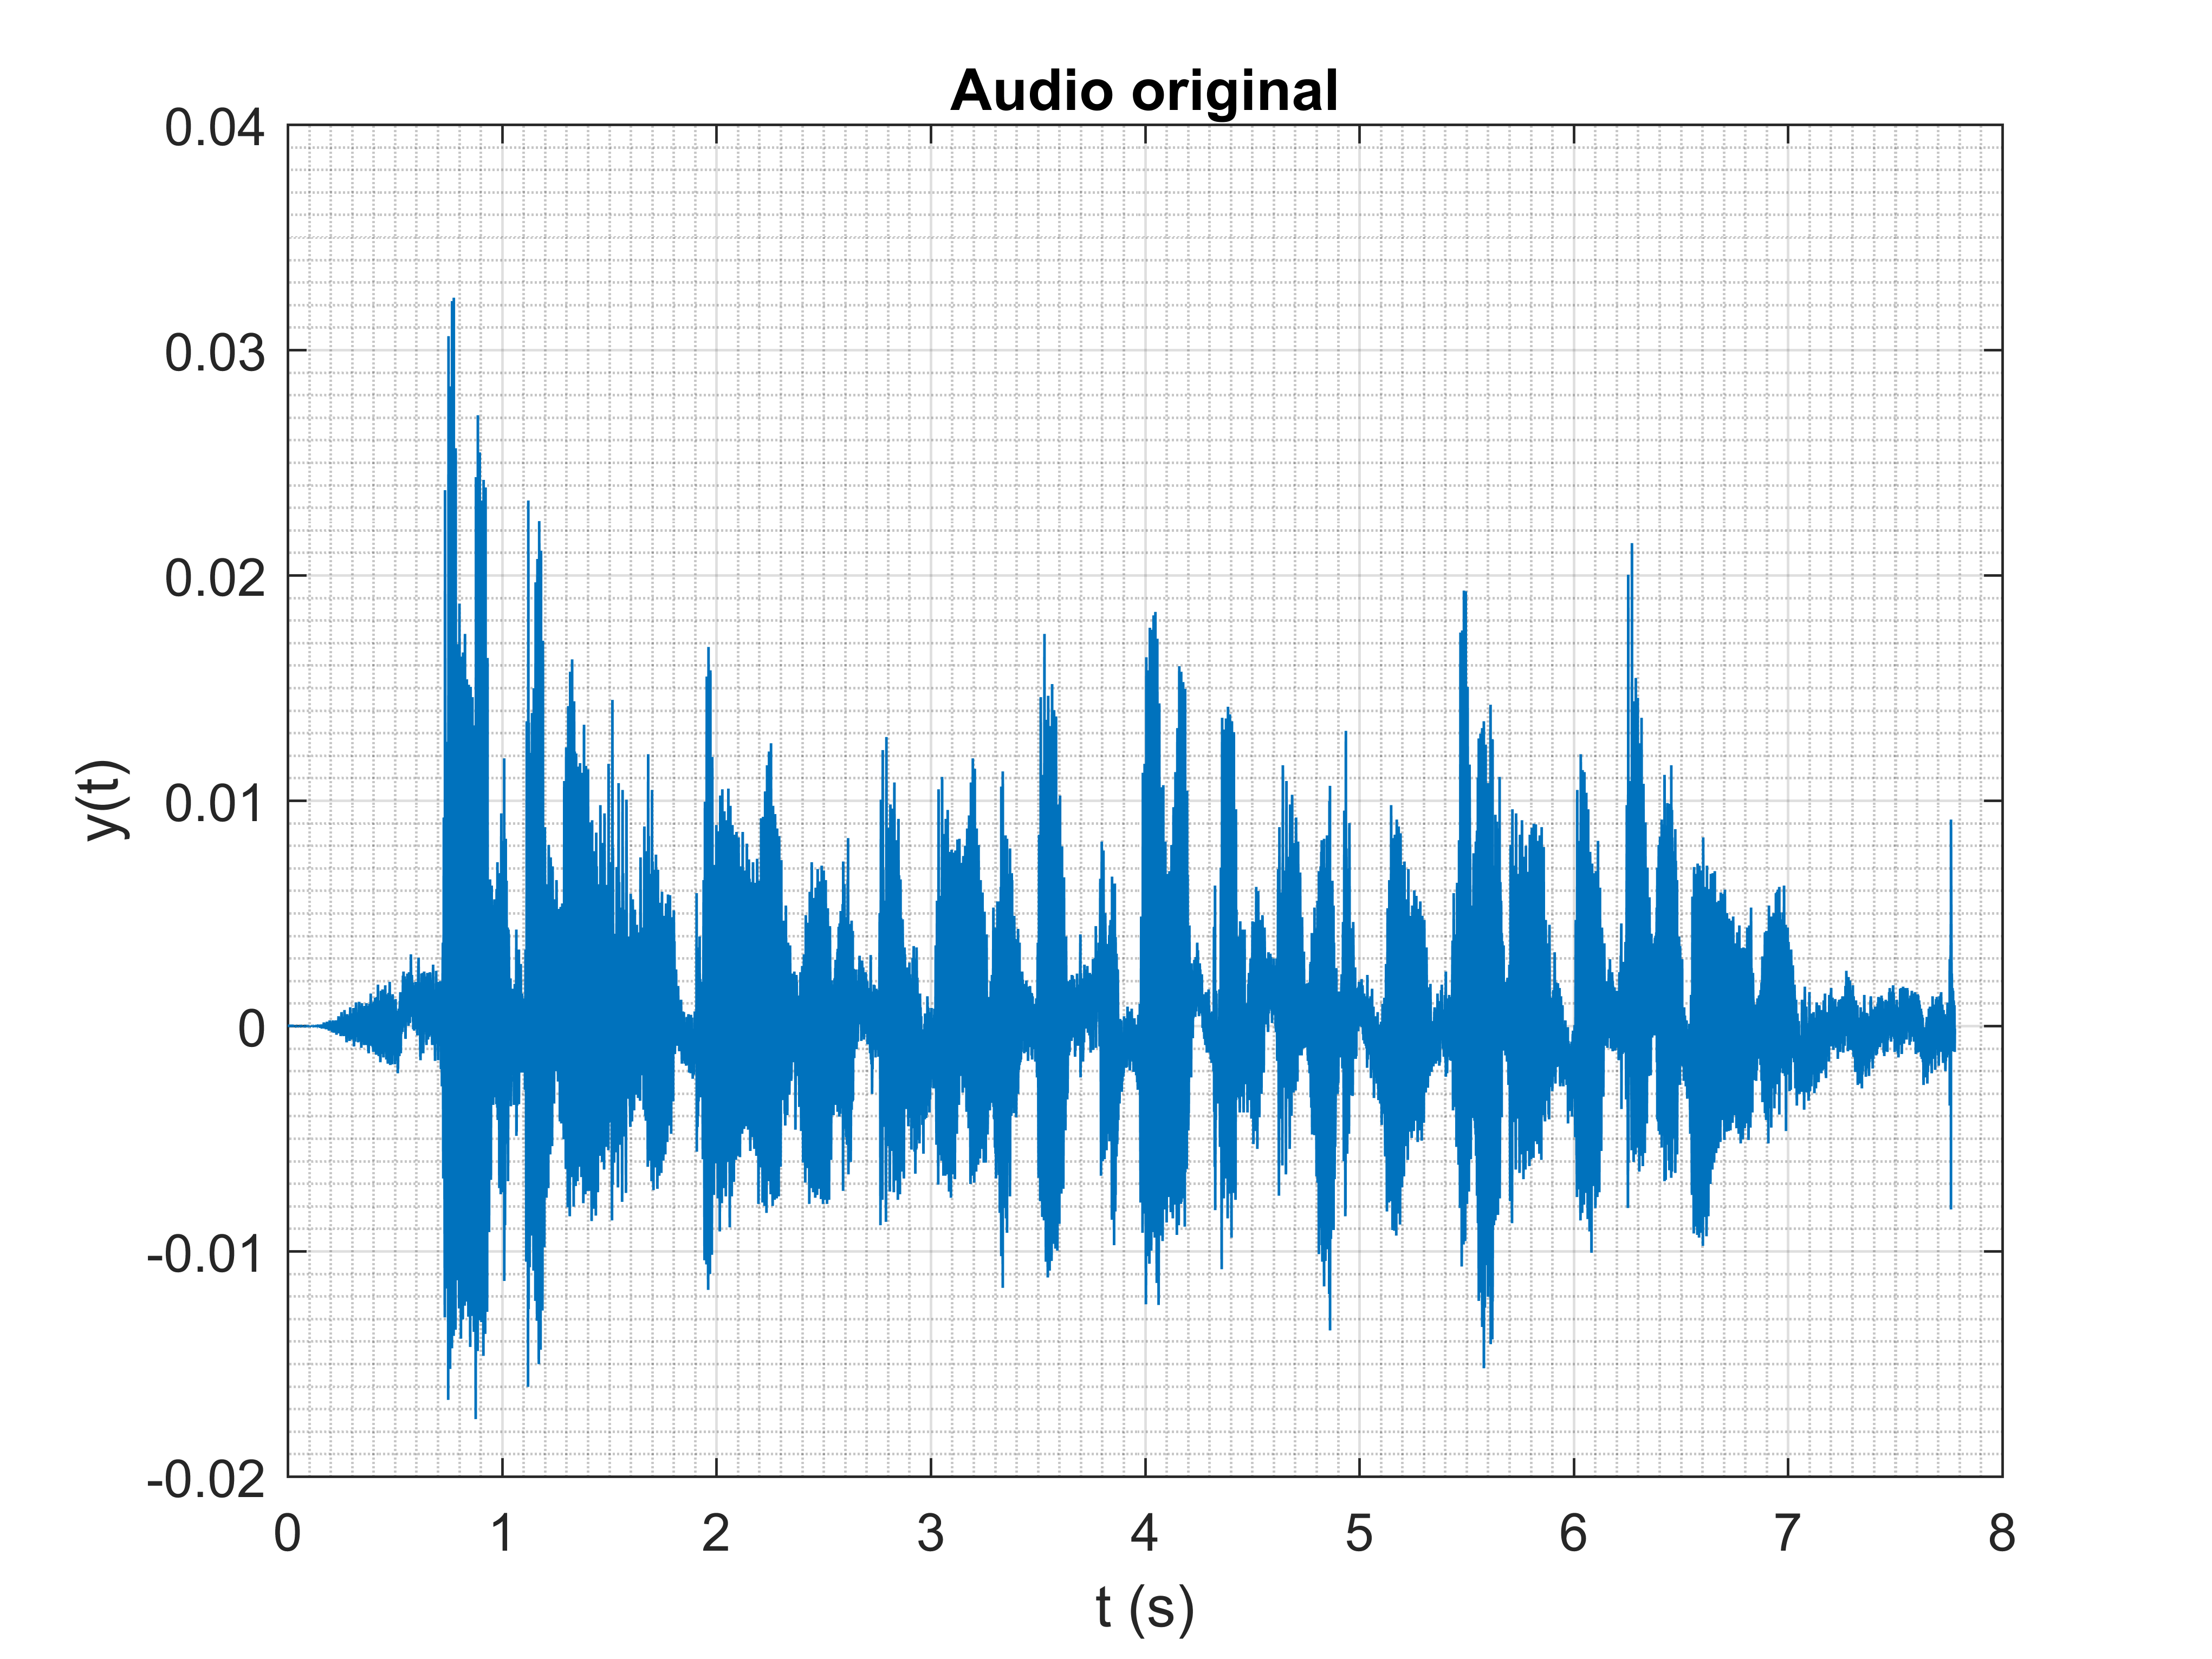
\includegraphics[scale=0.35]{graficos/audio_t.png}
        }
        \subfloat{
        \centering
        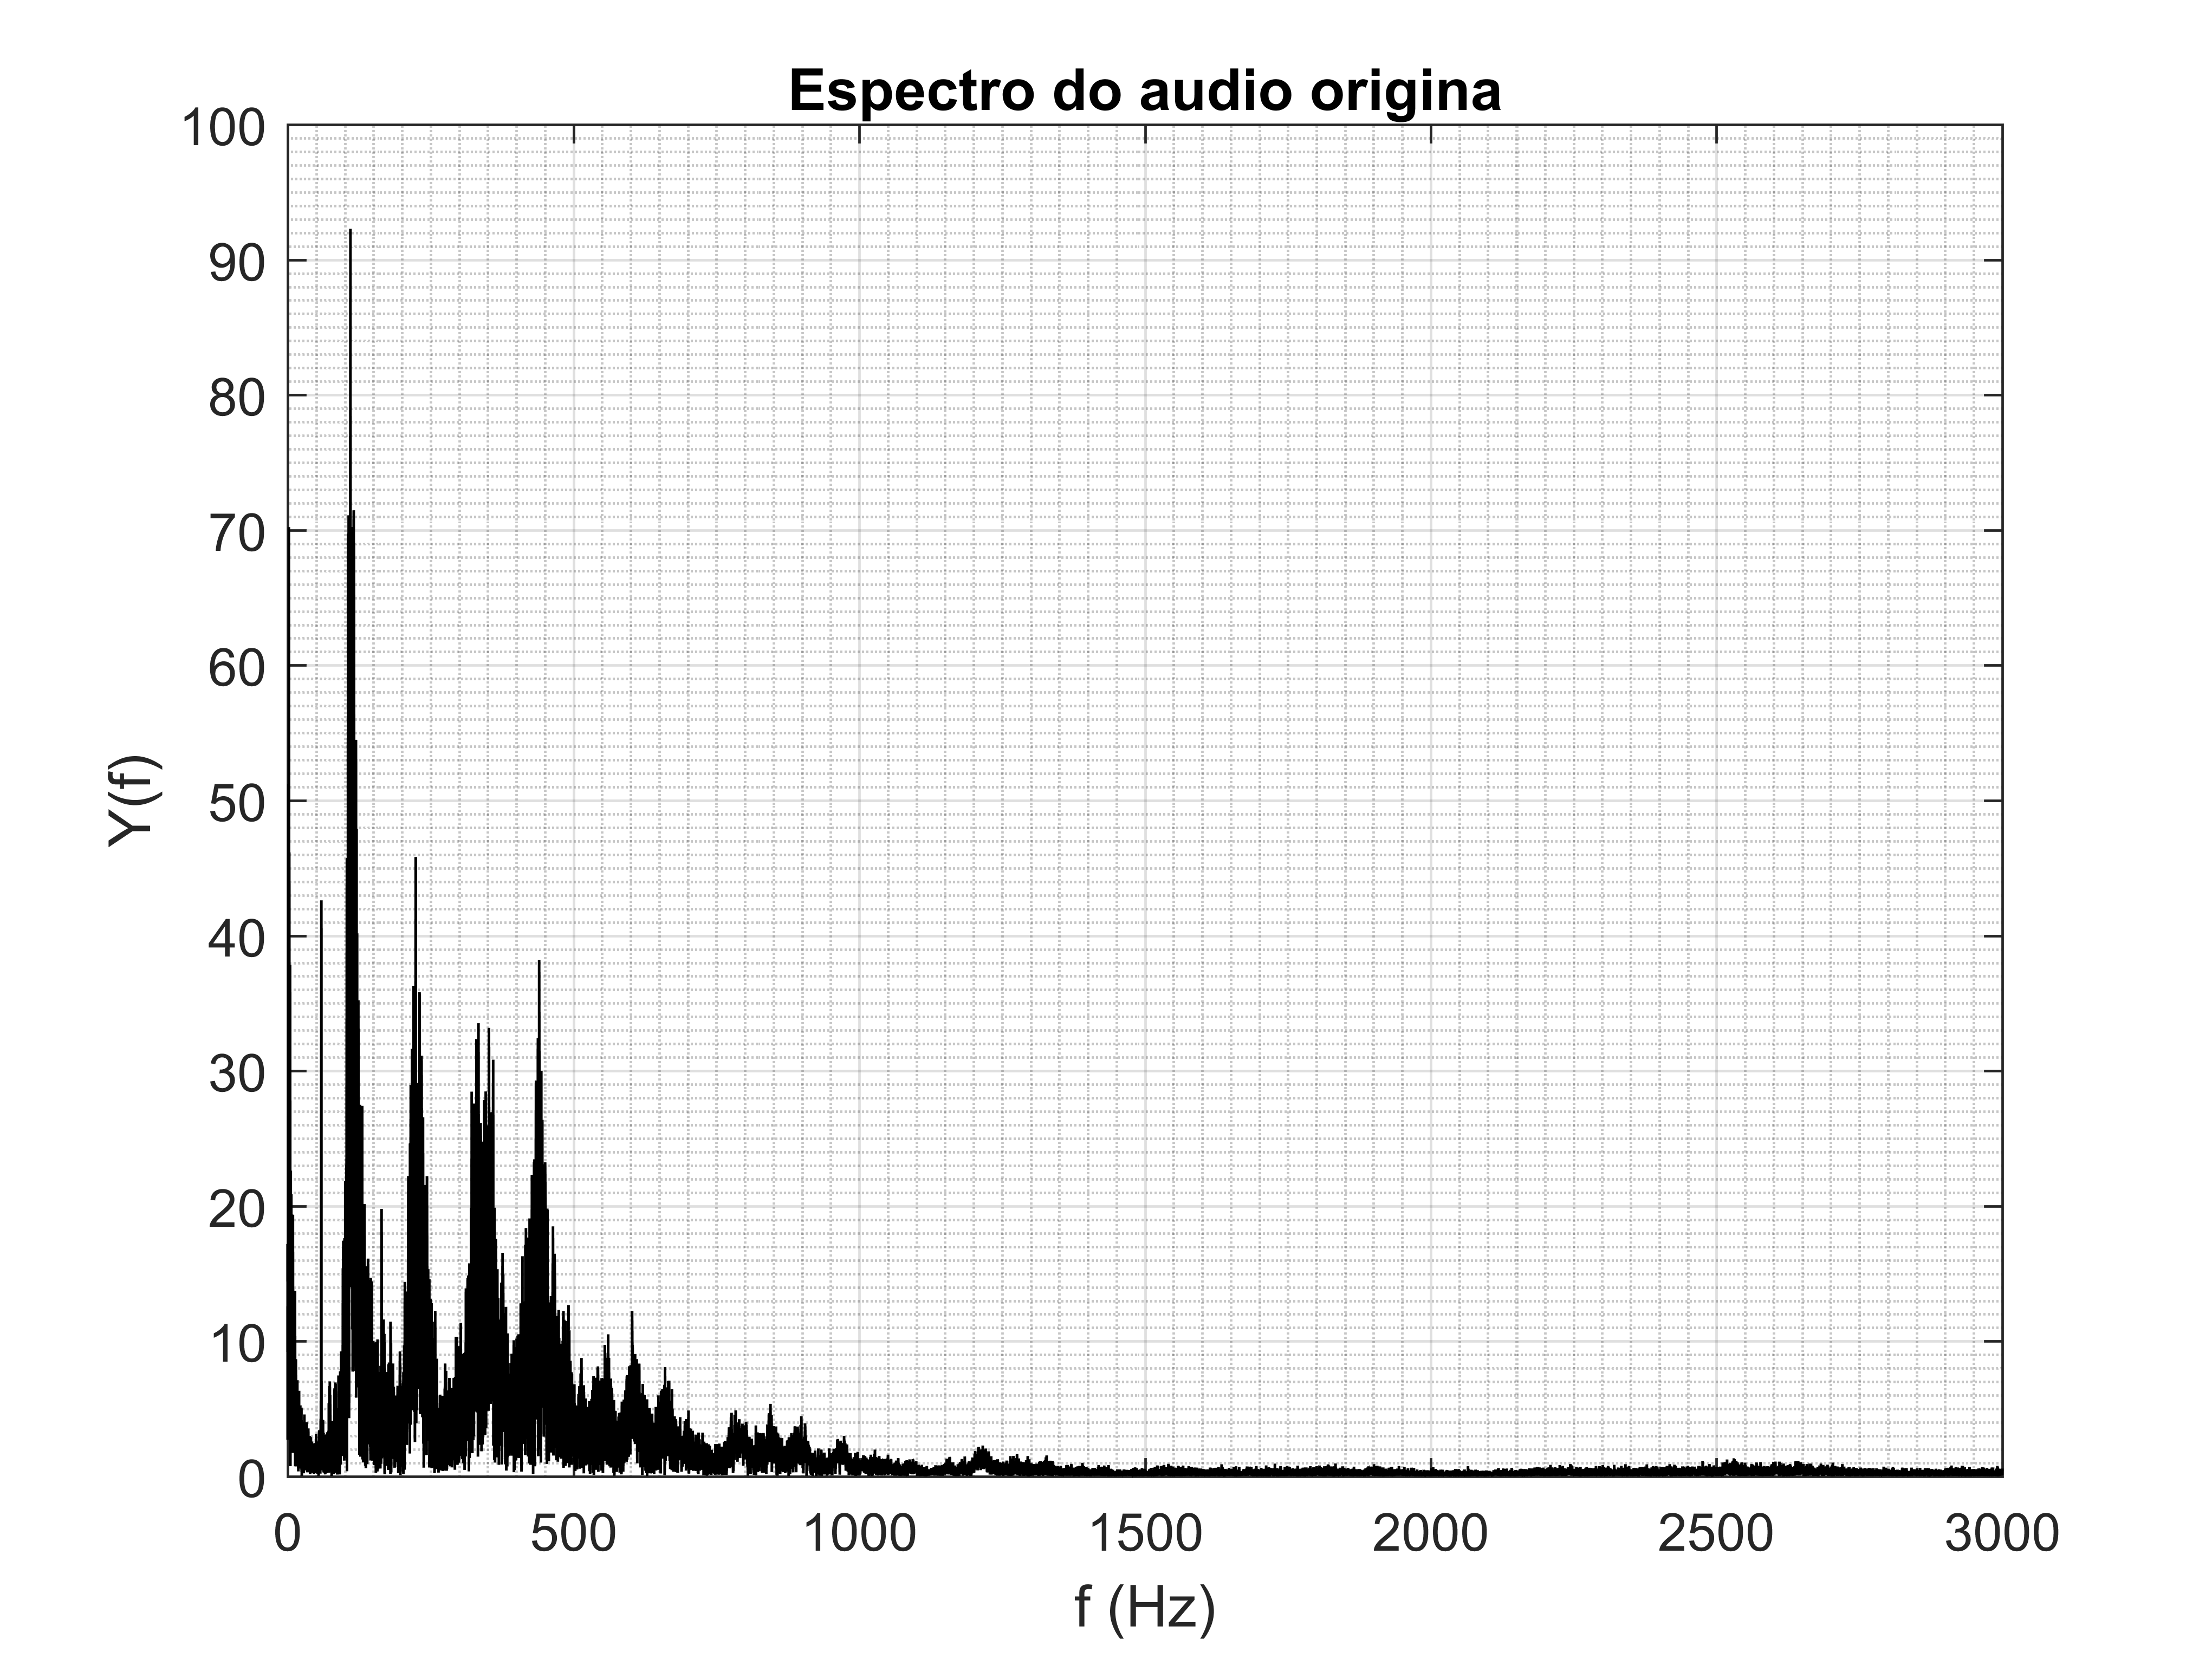
\includegraphics[scale=0.35]{graficos/audio_f.png}
        }
    \end{figure}   
\end{frame}

  

\begin{frame}{Ruído limitado em banda}
    \begin{figure}[!htb]
        \centering
        \subfloat{
        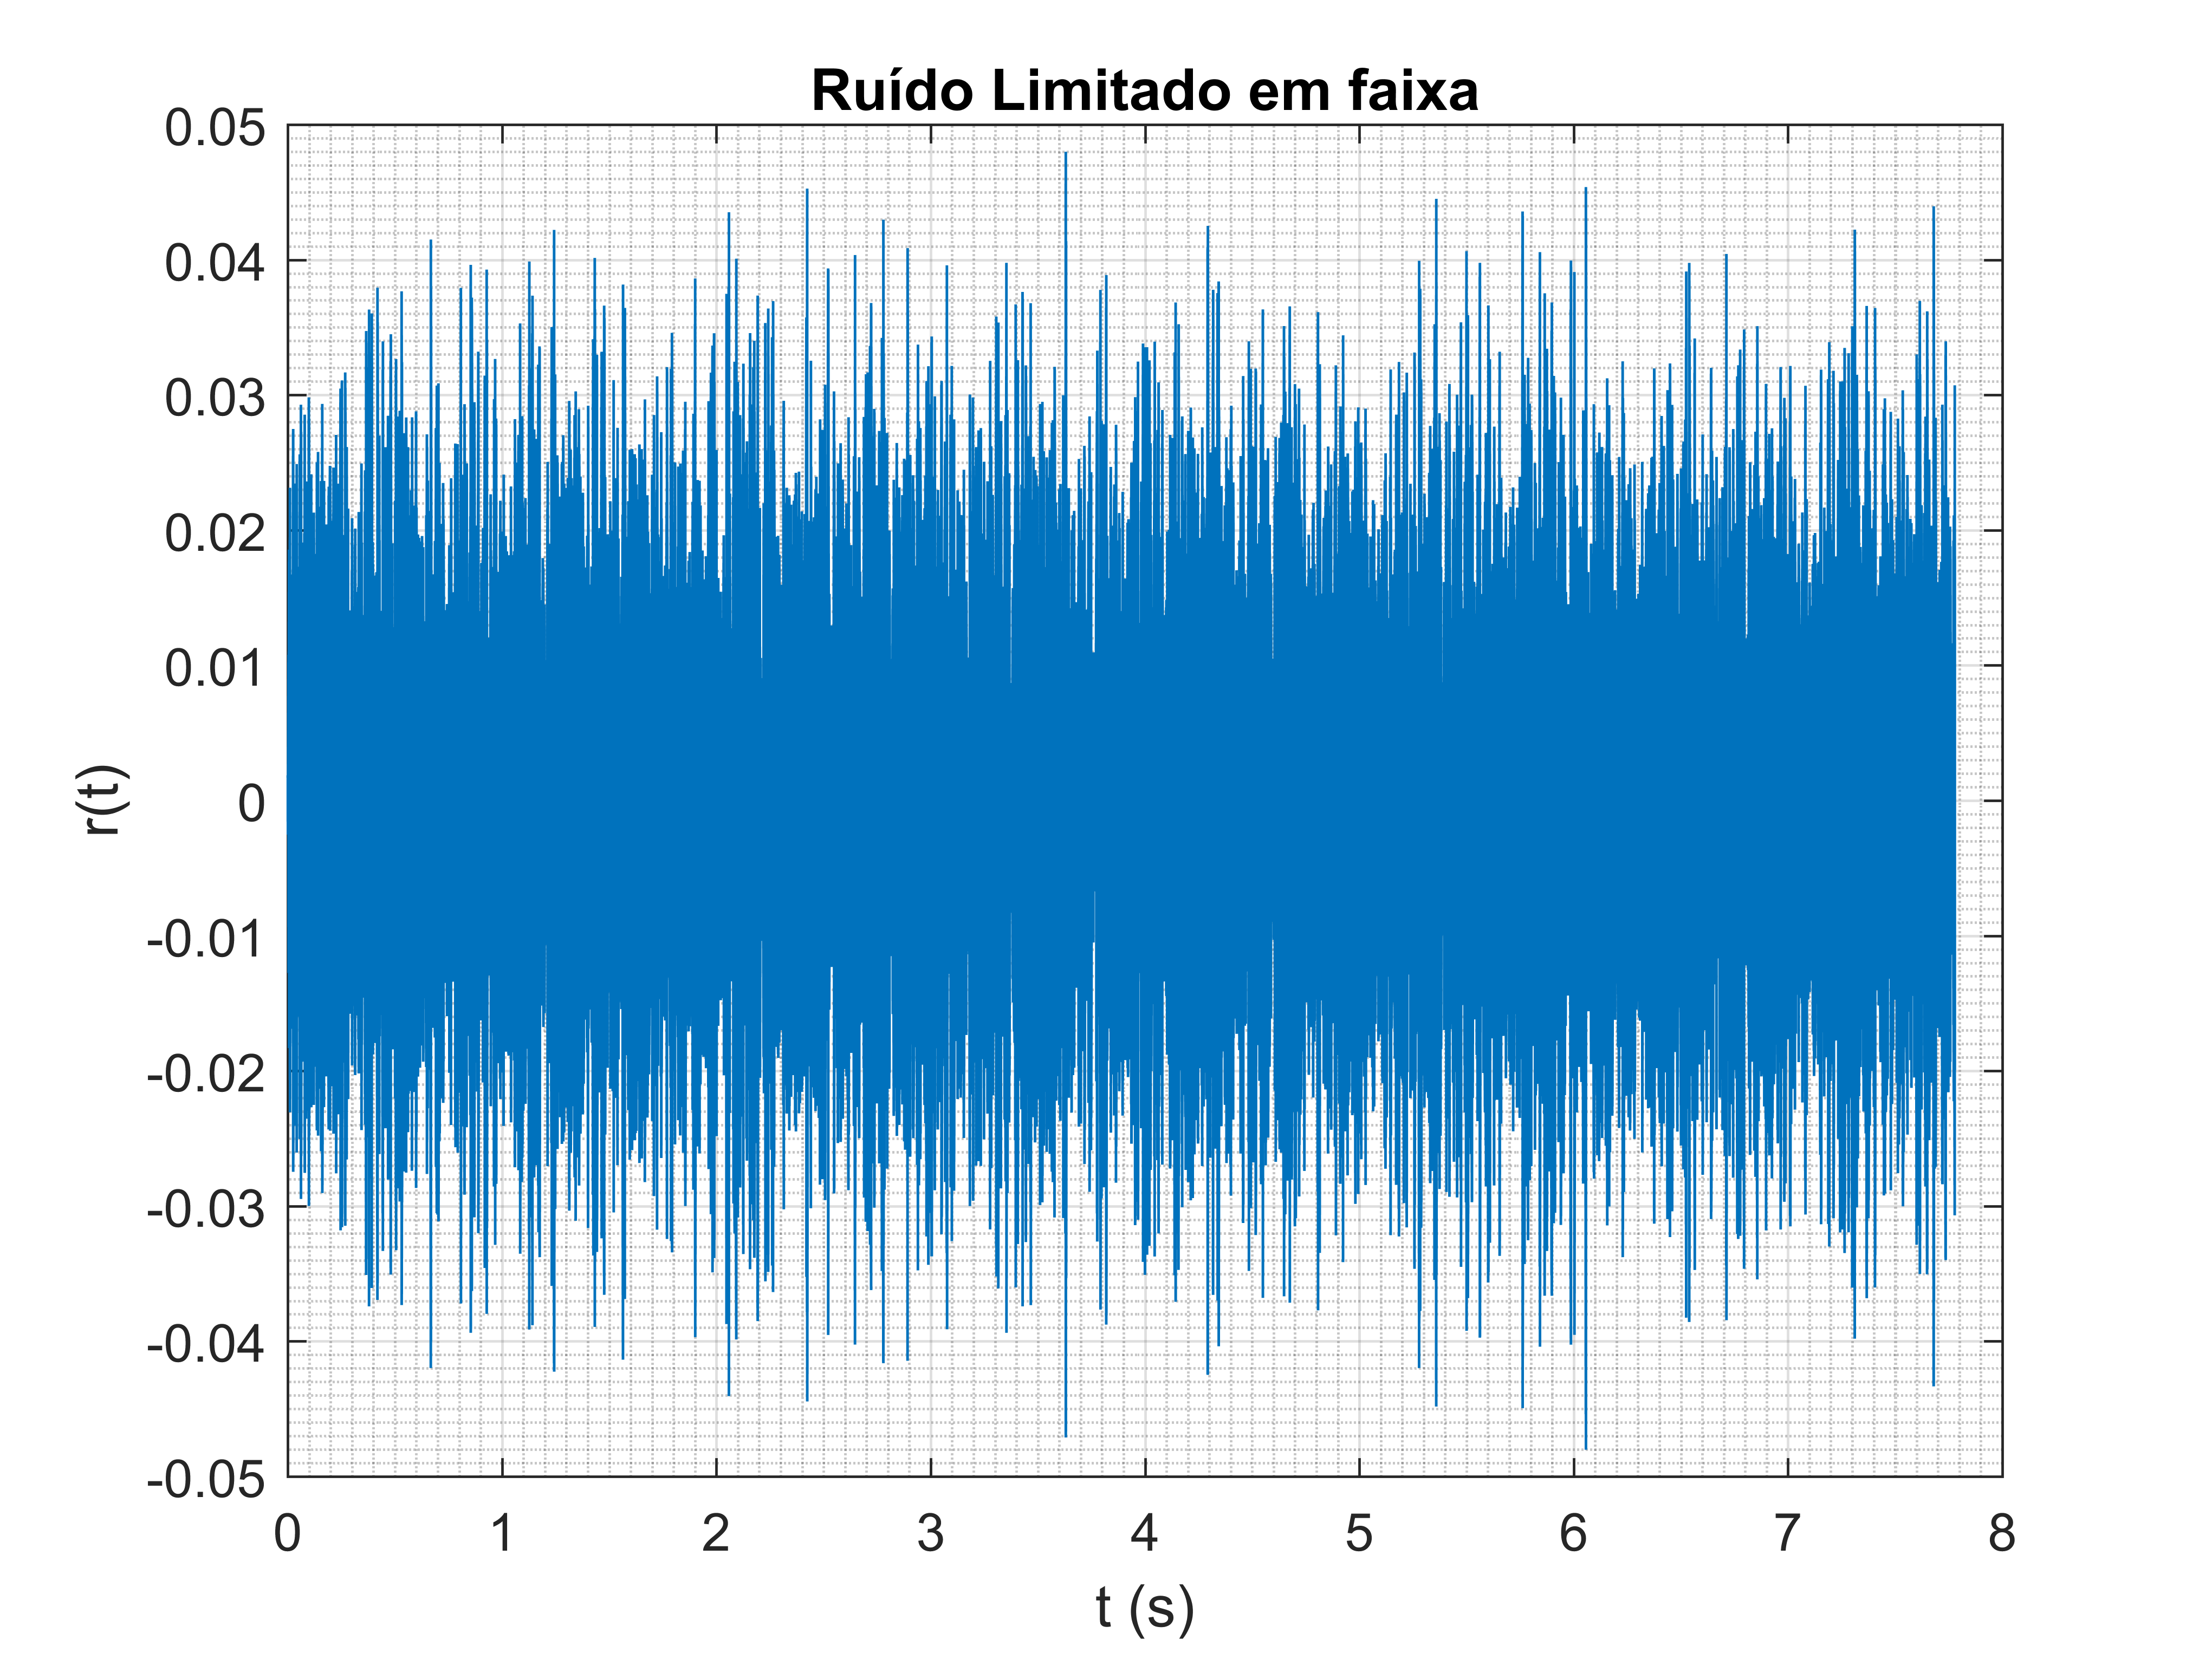
\includegraphics[scale=0.35]{graficos/ruido_limitado_t.png}
        }
        \subfloat{
        \centering
        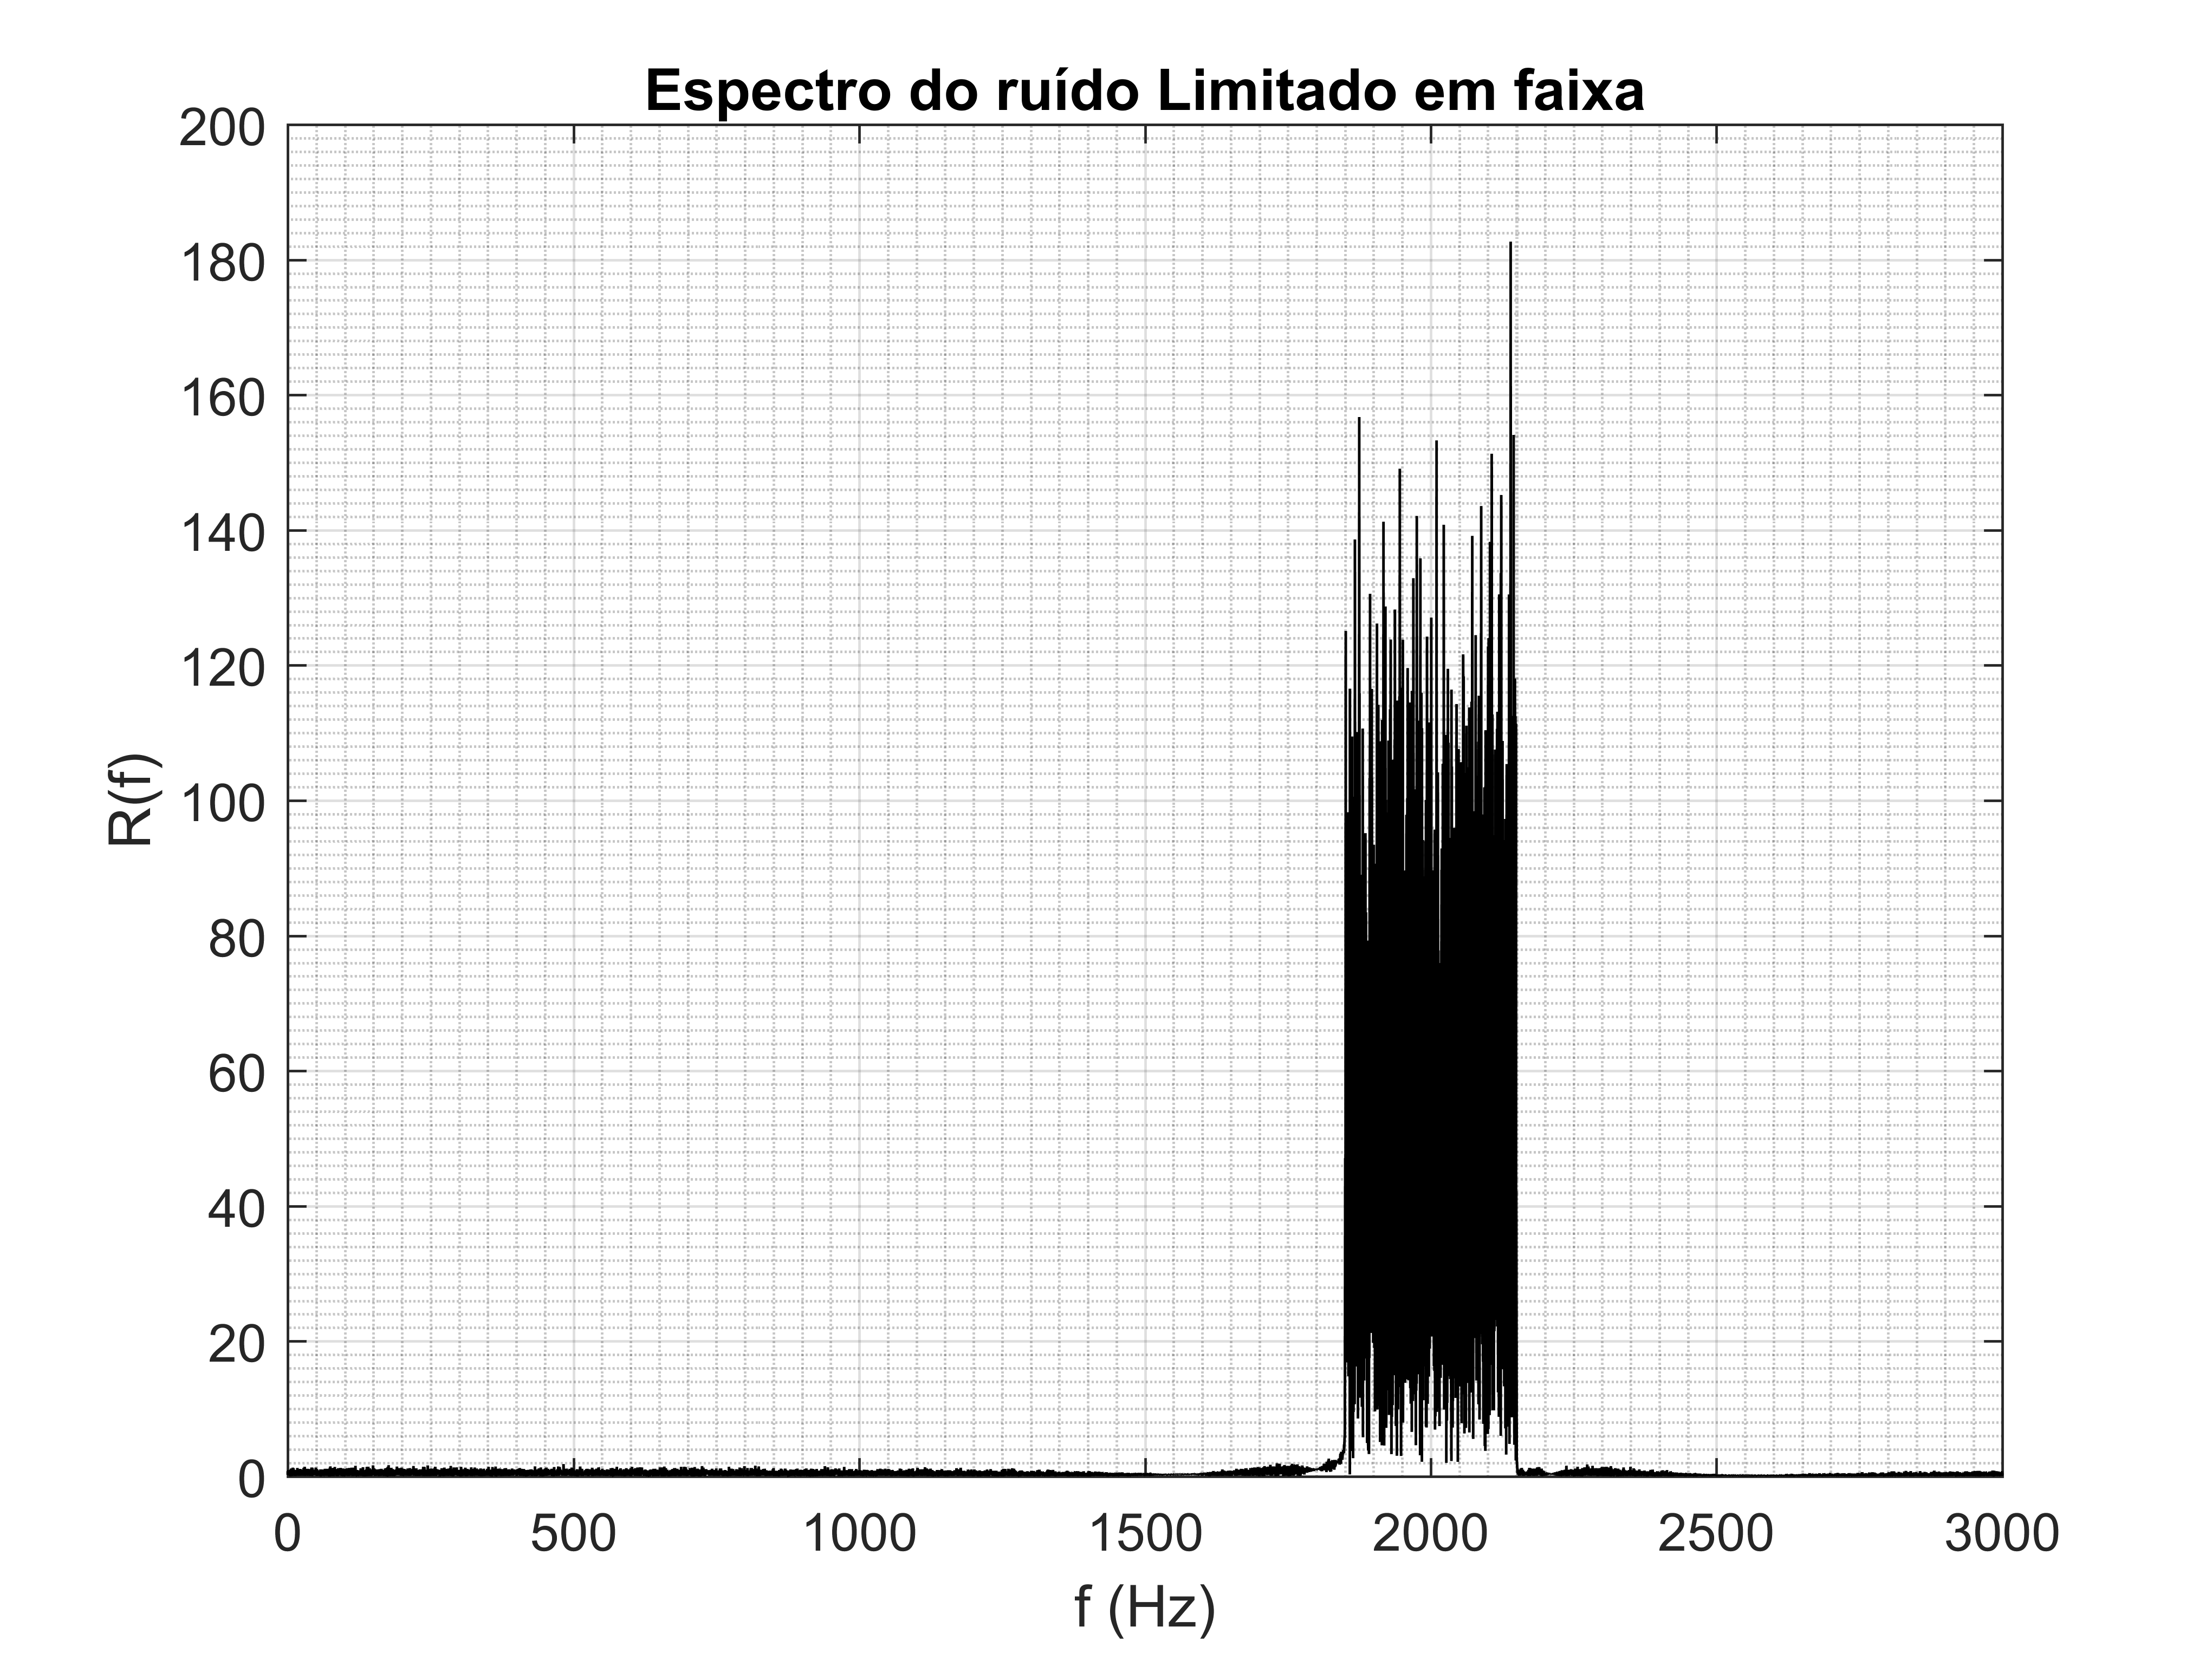
\includegraphics[scale=0.35]{graficos/ruido_limitado_f.png}
        }
    \end{figure}
    
\end{frame}

\begin{frame}{Áudio original corrompido pelo ruído}
    \begin{figure}[!htb]
        \centering
        \subfloat{
        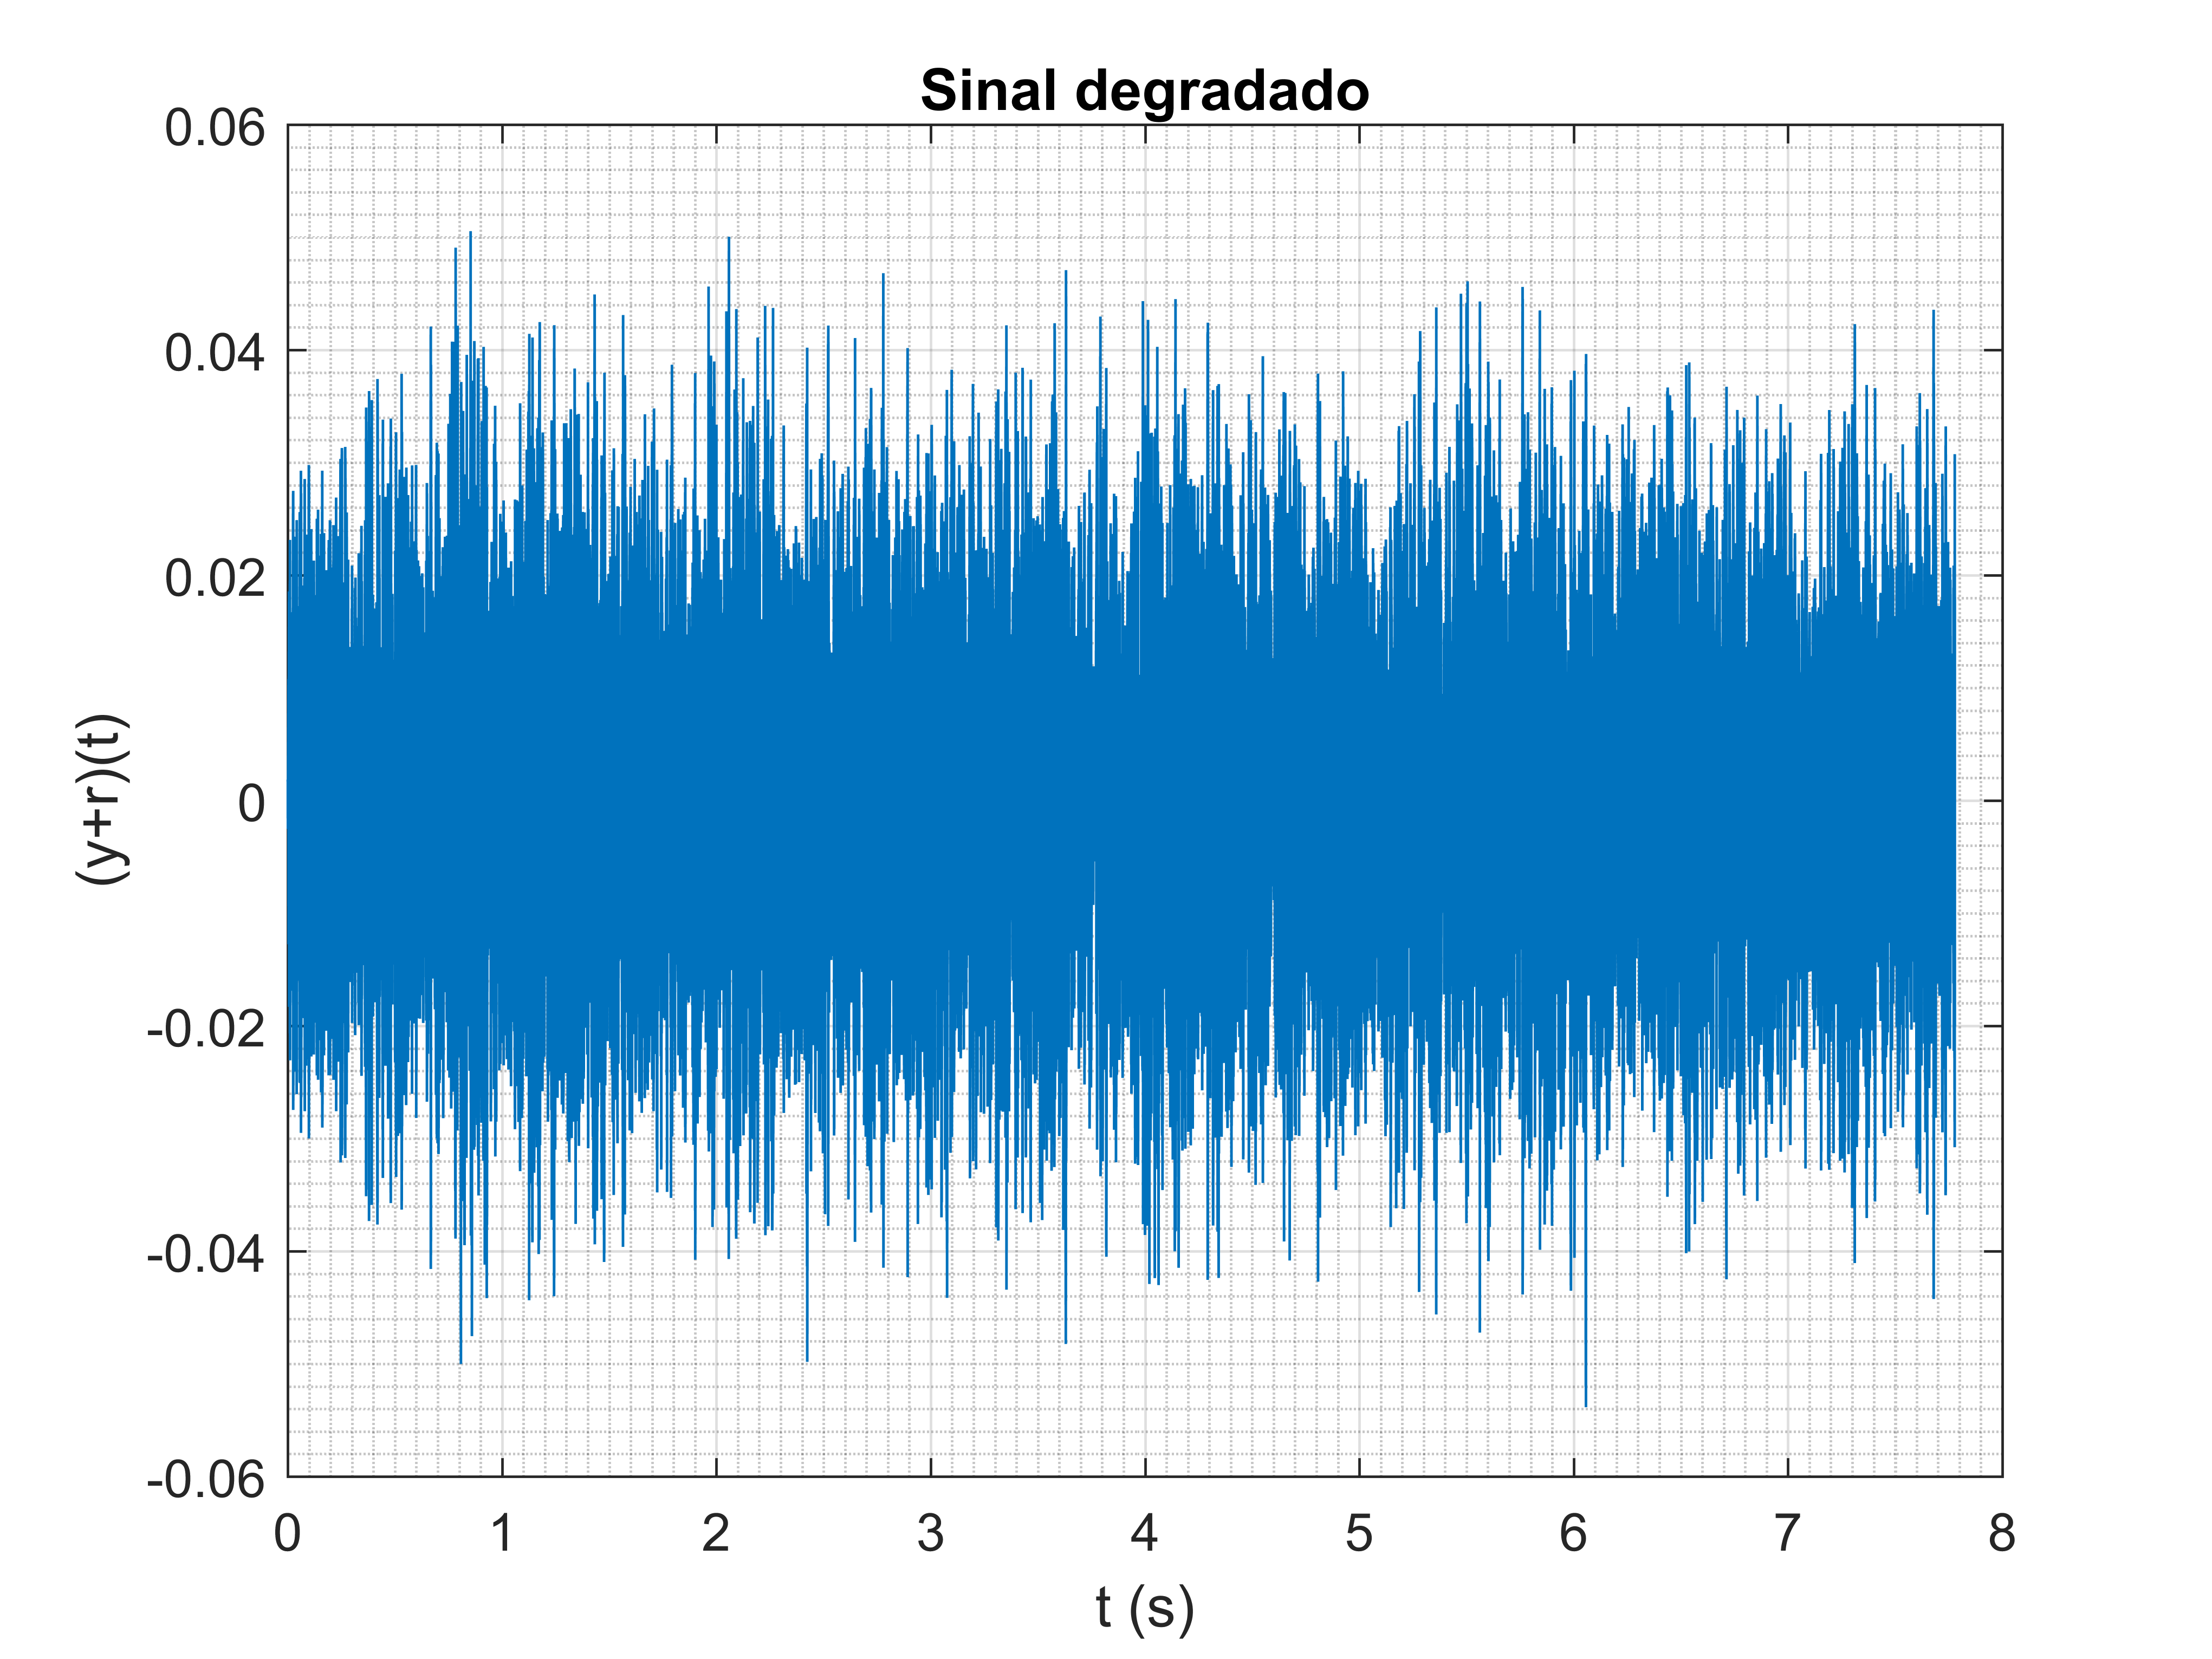
\includegraphics[scale=0.35]{graficos/sinal_ruido_t.png}
        }
        \subfloat{
        \centering
        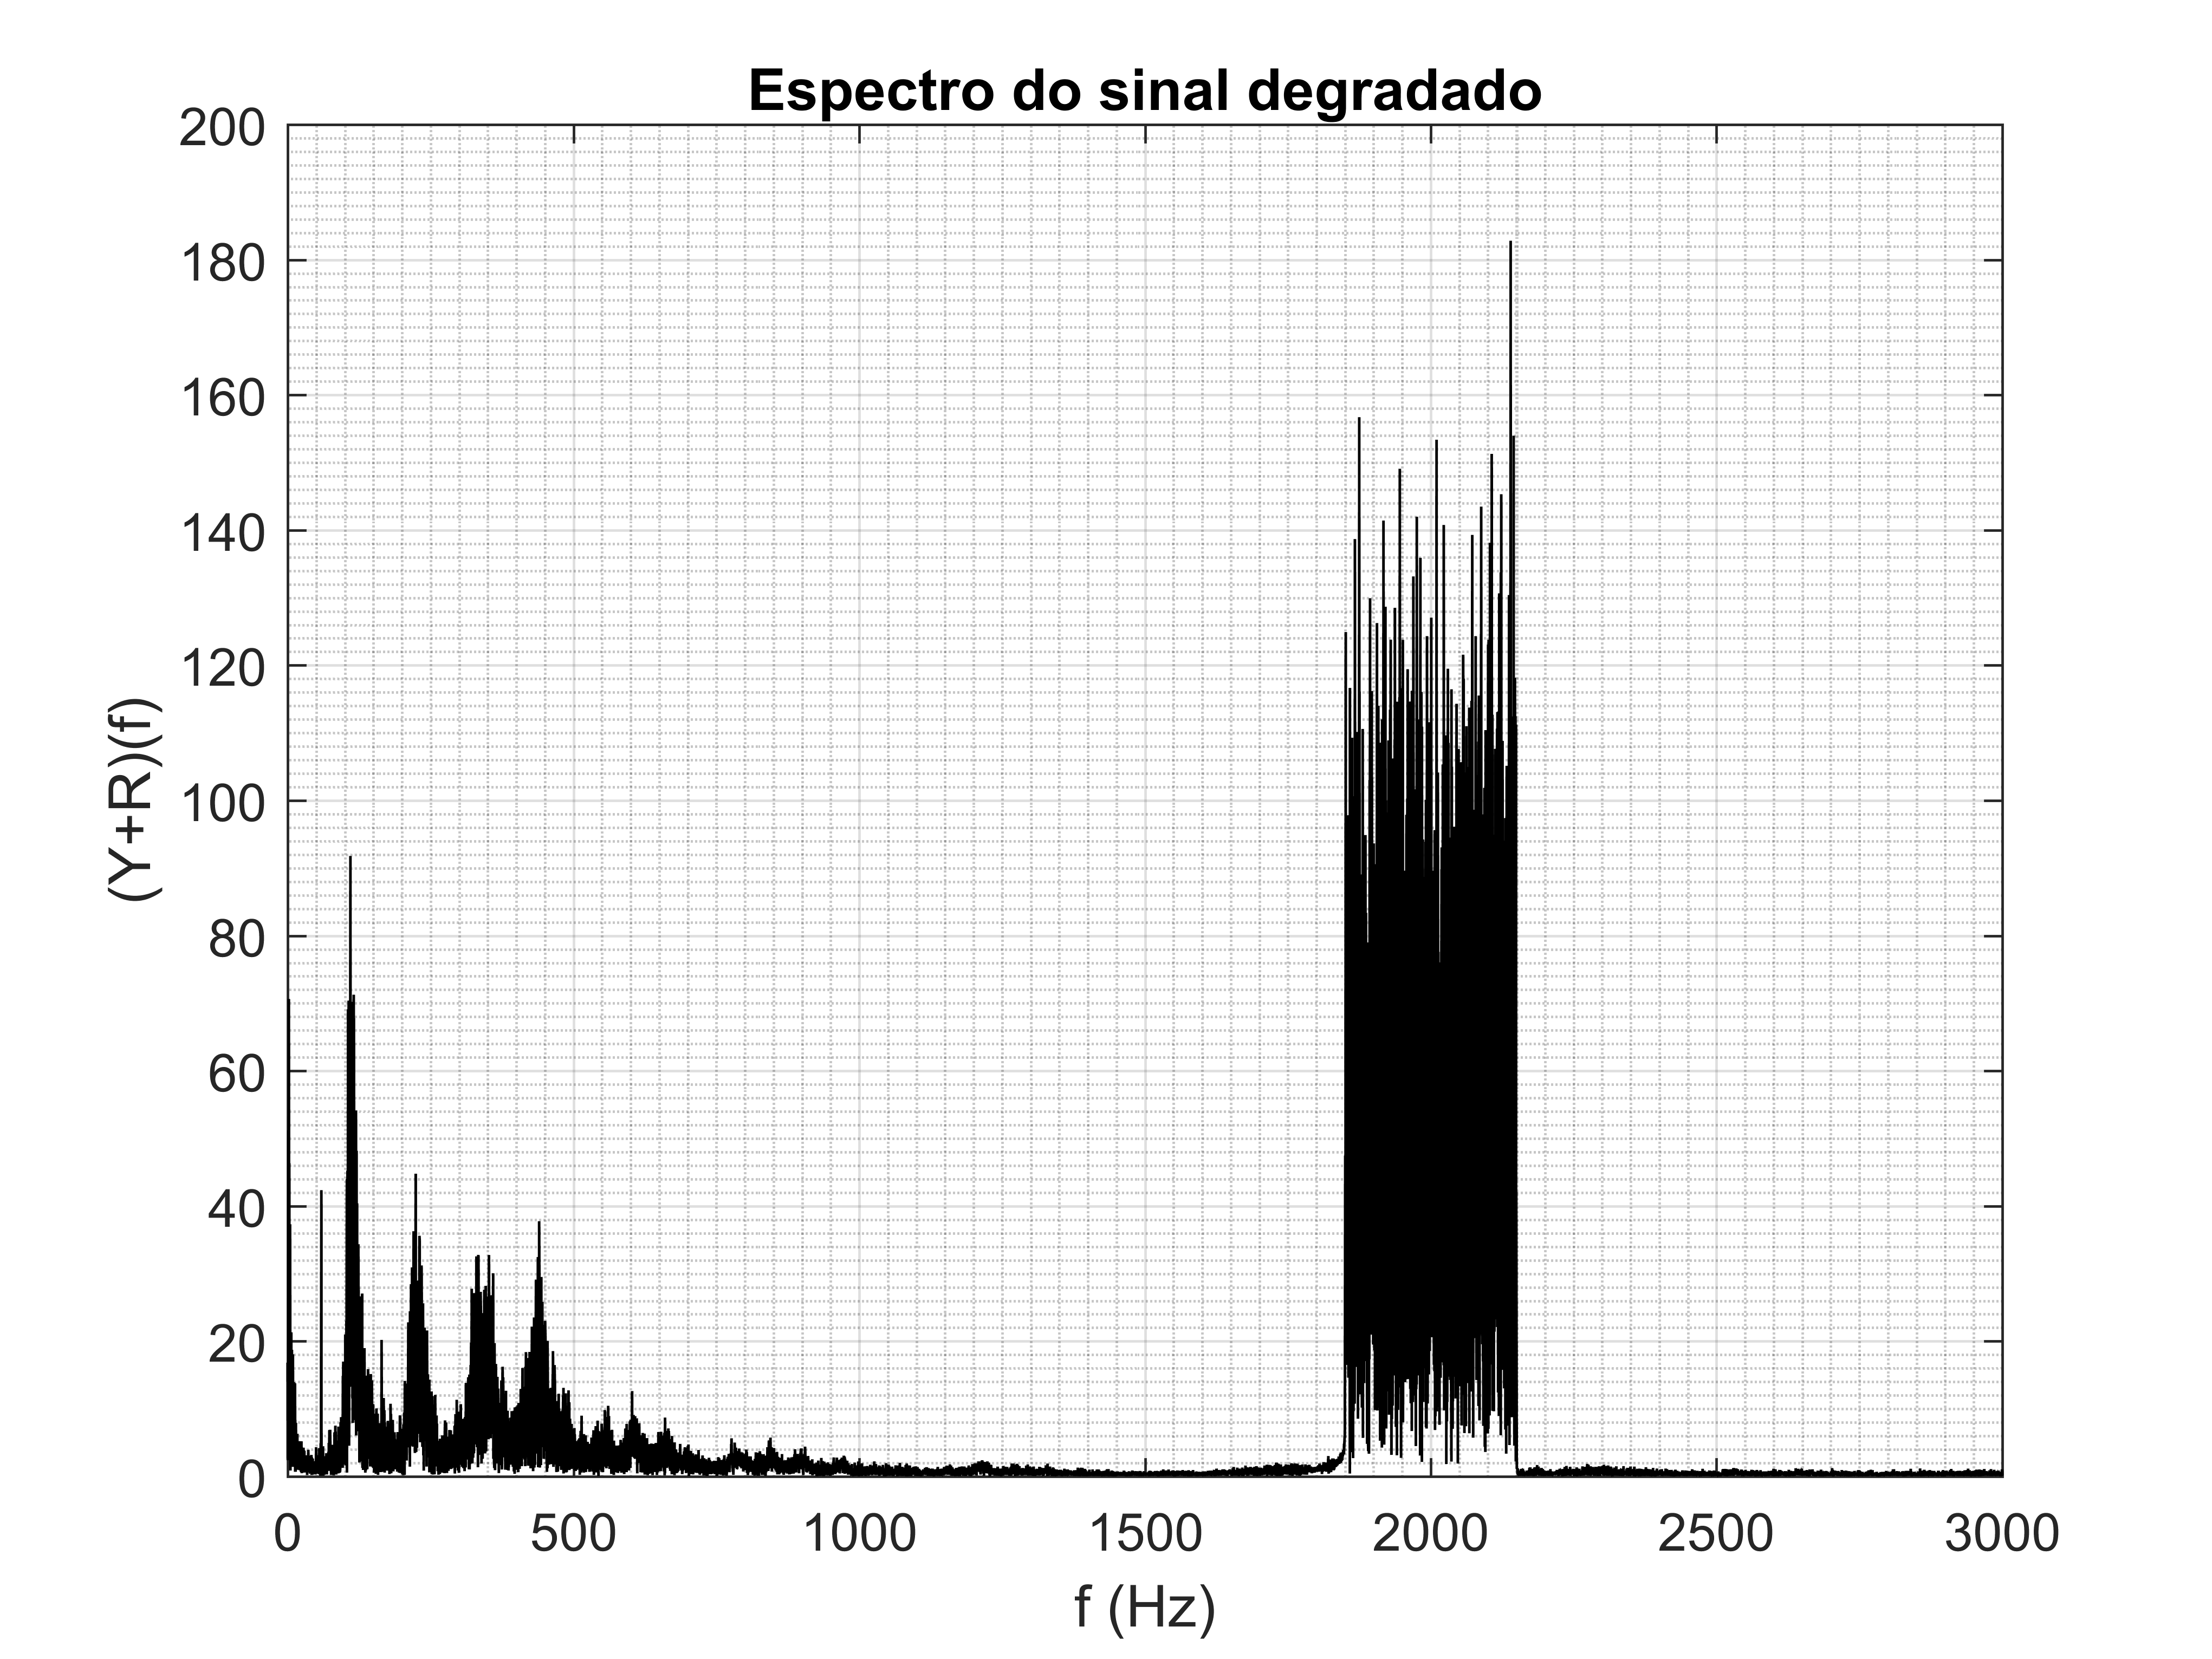
\includegraphics[scale=0.35]{graficos/sinal_ruido_f.png}
        }
    \end{figure}
\end{frame}


\begin{frame}{Especificações dos Filtros}
    \begin{itemize}
    \item Serão utilizadas 4 arquiteturas de filtros: Butterworth, Chebyshev I e II e Elíptico
        \item Os filtros serão passa-faixa com as especificações abaixo
            \begin{itemize}
                \item Limite da primeira faixa de passagem $\omega_{p1}$ = 2$\pi$1800
                \item Primeiro limite da faixa de rejeição $\omega_{s1}$ = 2$\pi$1850
                \item Segundo limite da faixa de rejeição $\omega_{p2}$ = 2$\pi$2150
                \item Limite da segunda faixa de passagem $\omega_{s2}$ = 2$\pi$2200
                \item Variação máxima de ganho nas faixas de passagem e transição $\epsilon$ = $\delta$ = 0.01 
            \end{itemize}
        
        \item Projetados usando técnicas de filtros analógicos
        
        \item Posteriormente discretizados usando transformação bilinear  
        
    \end{itemize}
\end{frame}

\begin{frame}{Especificações dos Filtros}
    \begin{figure}[!htb]
        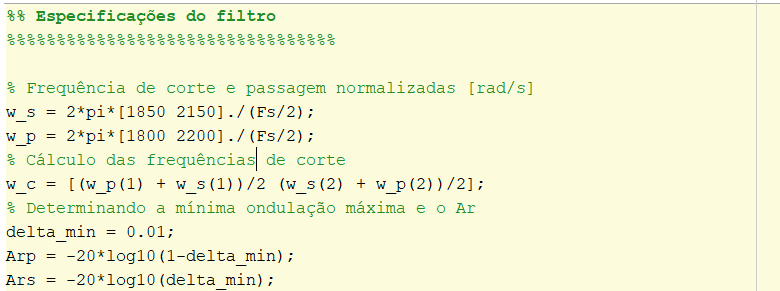
\includegraphics[width=0.9\textwidth]{graficos/especificacoes.png}
        \end{figure} 
\end{frame}

\begin{frame}{Gabarito do Filtro}
    	\begin{figure}[!htb]
        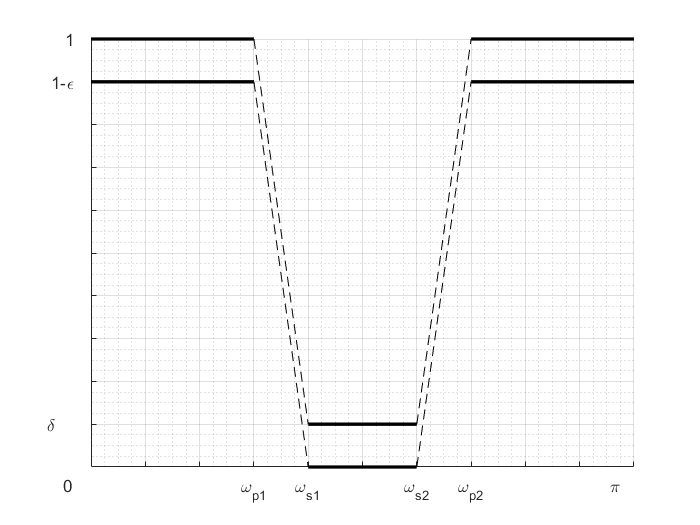
\includegraphics[width=0.7\textwidth]{graficos/gabarito.png}
        \end{figure} 
\end{frame}

\begin{frame}{Tentativa 1 de cálculo de H(s)=N(s)/D(s)}
\begin{itemize}
    \item A ordem do primeiro filtro (Butterworth) foi de 50
    \item Não foi possível representar adequadamente os polinômios
    
\end{itemize}
    \begin{figure}[!htb]
    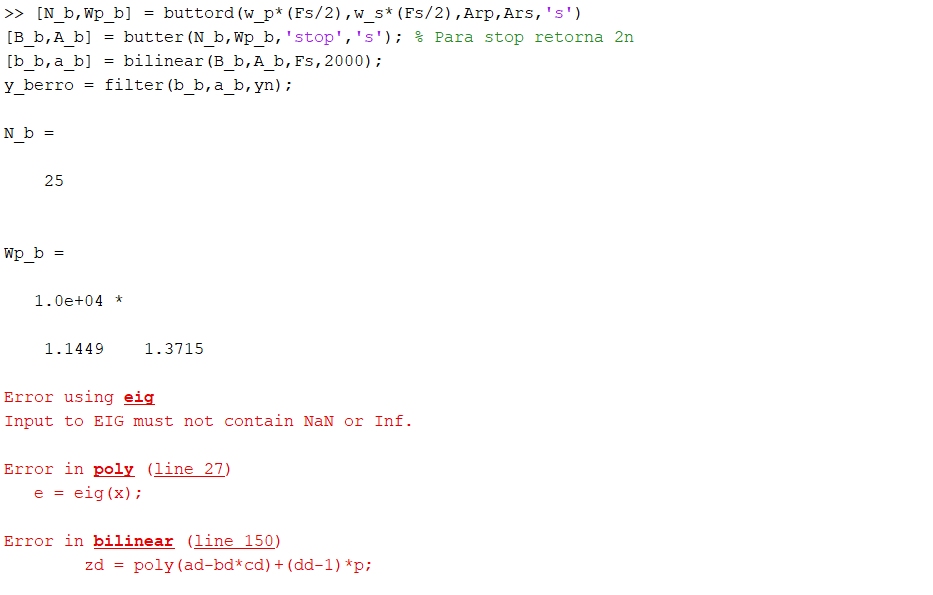
\includegraphics[width=0.6\textwidth]{graficos/num_dem_try_1_erro.png}
    \end{figure}
    
\end{frame}

\begin{frame}{Tentativa 1 de cálculo de H(s)=N(s)/D(s)}
        \begin{figure}[!htb]
        \centering
        \subfloat{
        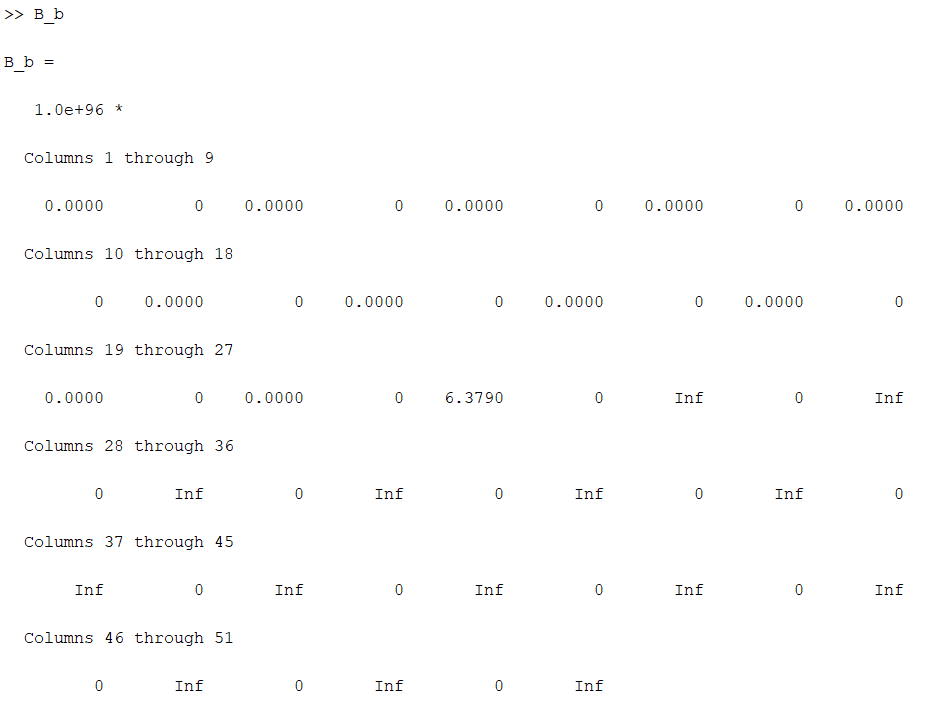
\includegraphics[scale=0.28]{graficos/num_dem_try_1_zeros.png}
        }
        \subfloat{
        \centering
        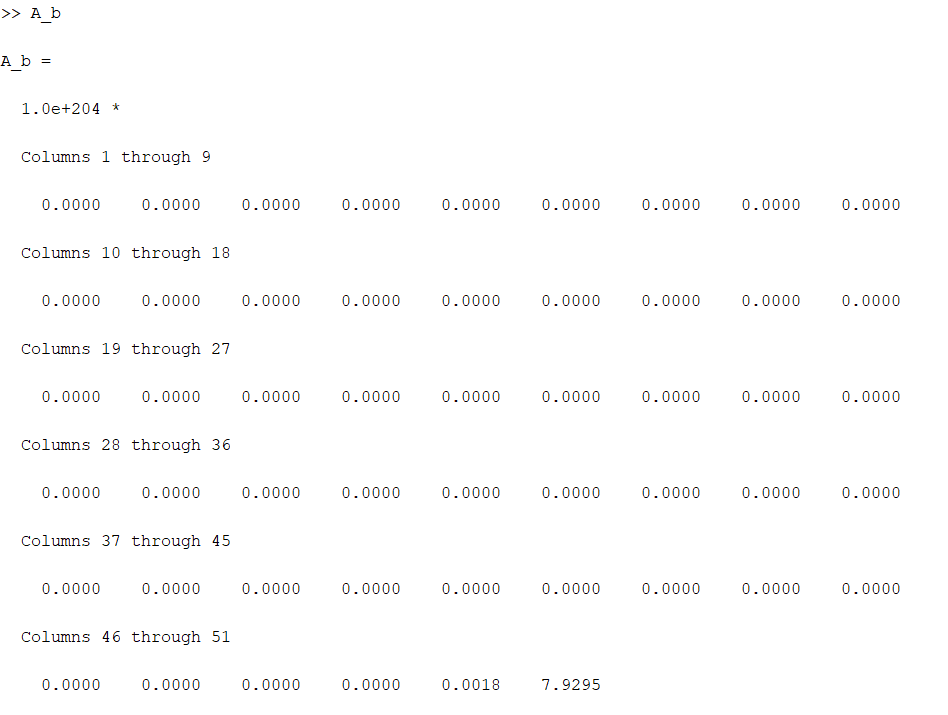
\includegraphics[scale=0.28]{graficos/num_dem_try_1_polos.png}
        }
    \end{figure}
\end{frame}

\begin{frame}{Tentativa 2 de cálculo de H(s)=N(s)/D(s)}
    \begin{itemize}
        \item Numa segunda tentativa foram calculados pólos e zeros fatorados
        \item Os pólos/zeros obtidos estavam no SPE (estáveis/fase mínima)
        \item Converteu-se estes pólos/zeros num polinômio D(s) e outro N(s)
        \item Novamente o polinômio obtido não representava adequadamente o filtro desejado
        \item Vários dos pólos/zeros do novo polinômio passaram a se localizar no SPD (instáveis/fase não-mínima)
    \end{itemize}
\end{frame}

\begin{frame}{Tentativa 2 de cálculo de H(s)=N(s)/D(s)}
    O diagrama de pólos e zeros mostra onde estavam os pólos e zeros originais (vermelhos) e onde passaram a ficar após serem tranformados em um polinômio de ordem alta (pretos)
    \begin{figure}[!htb]
    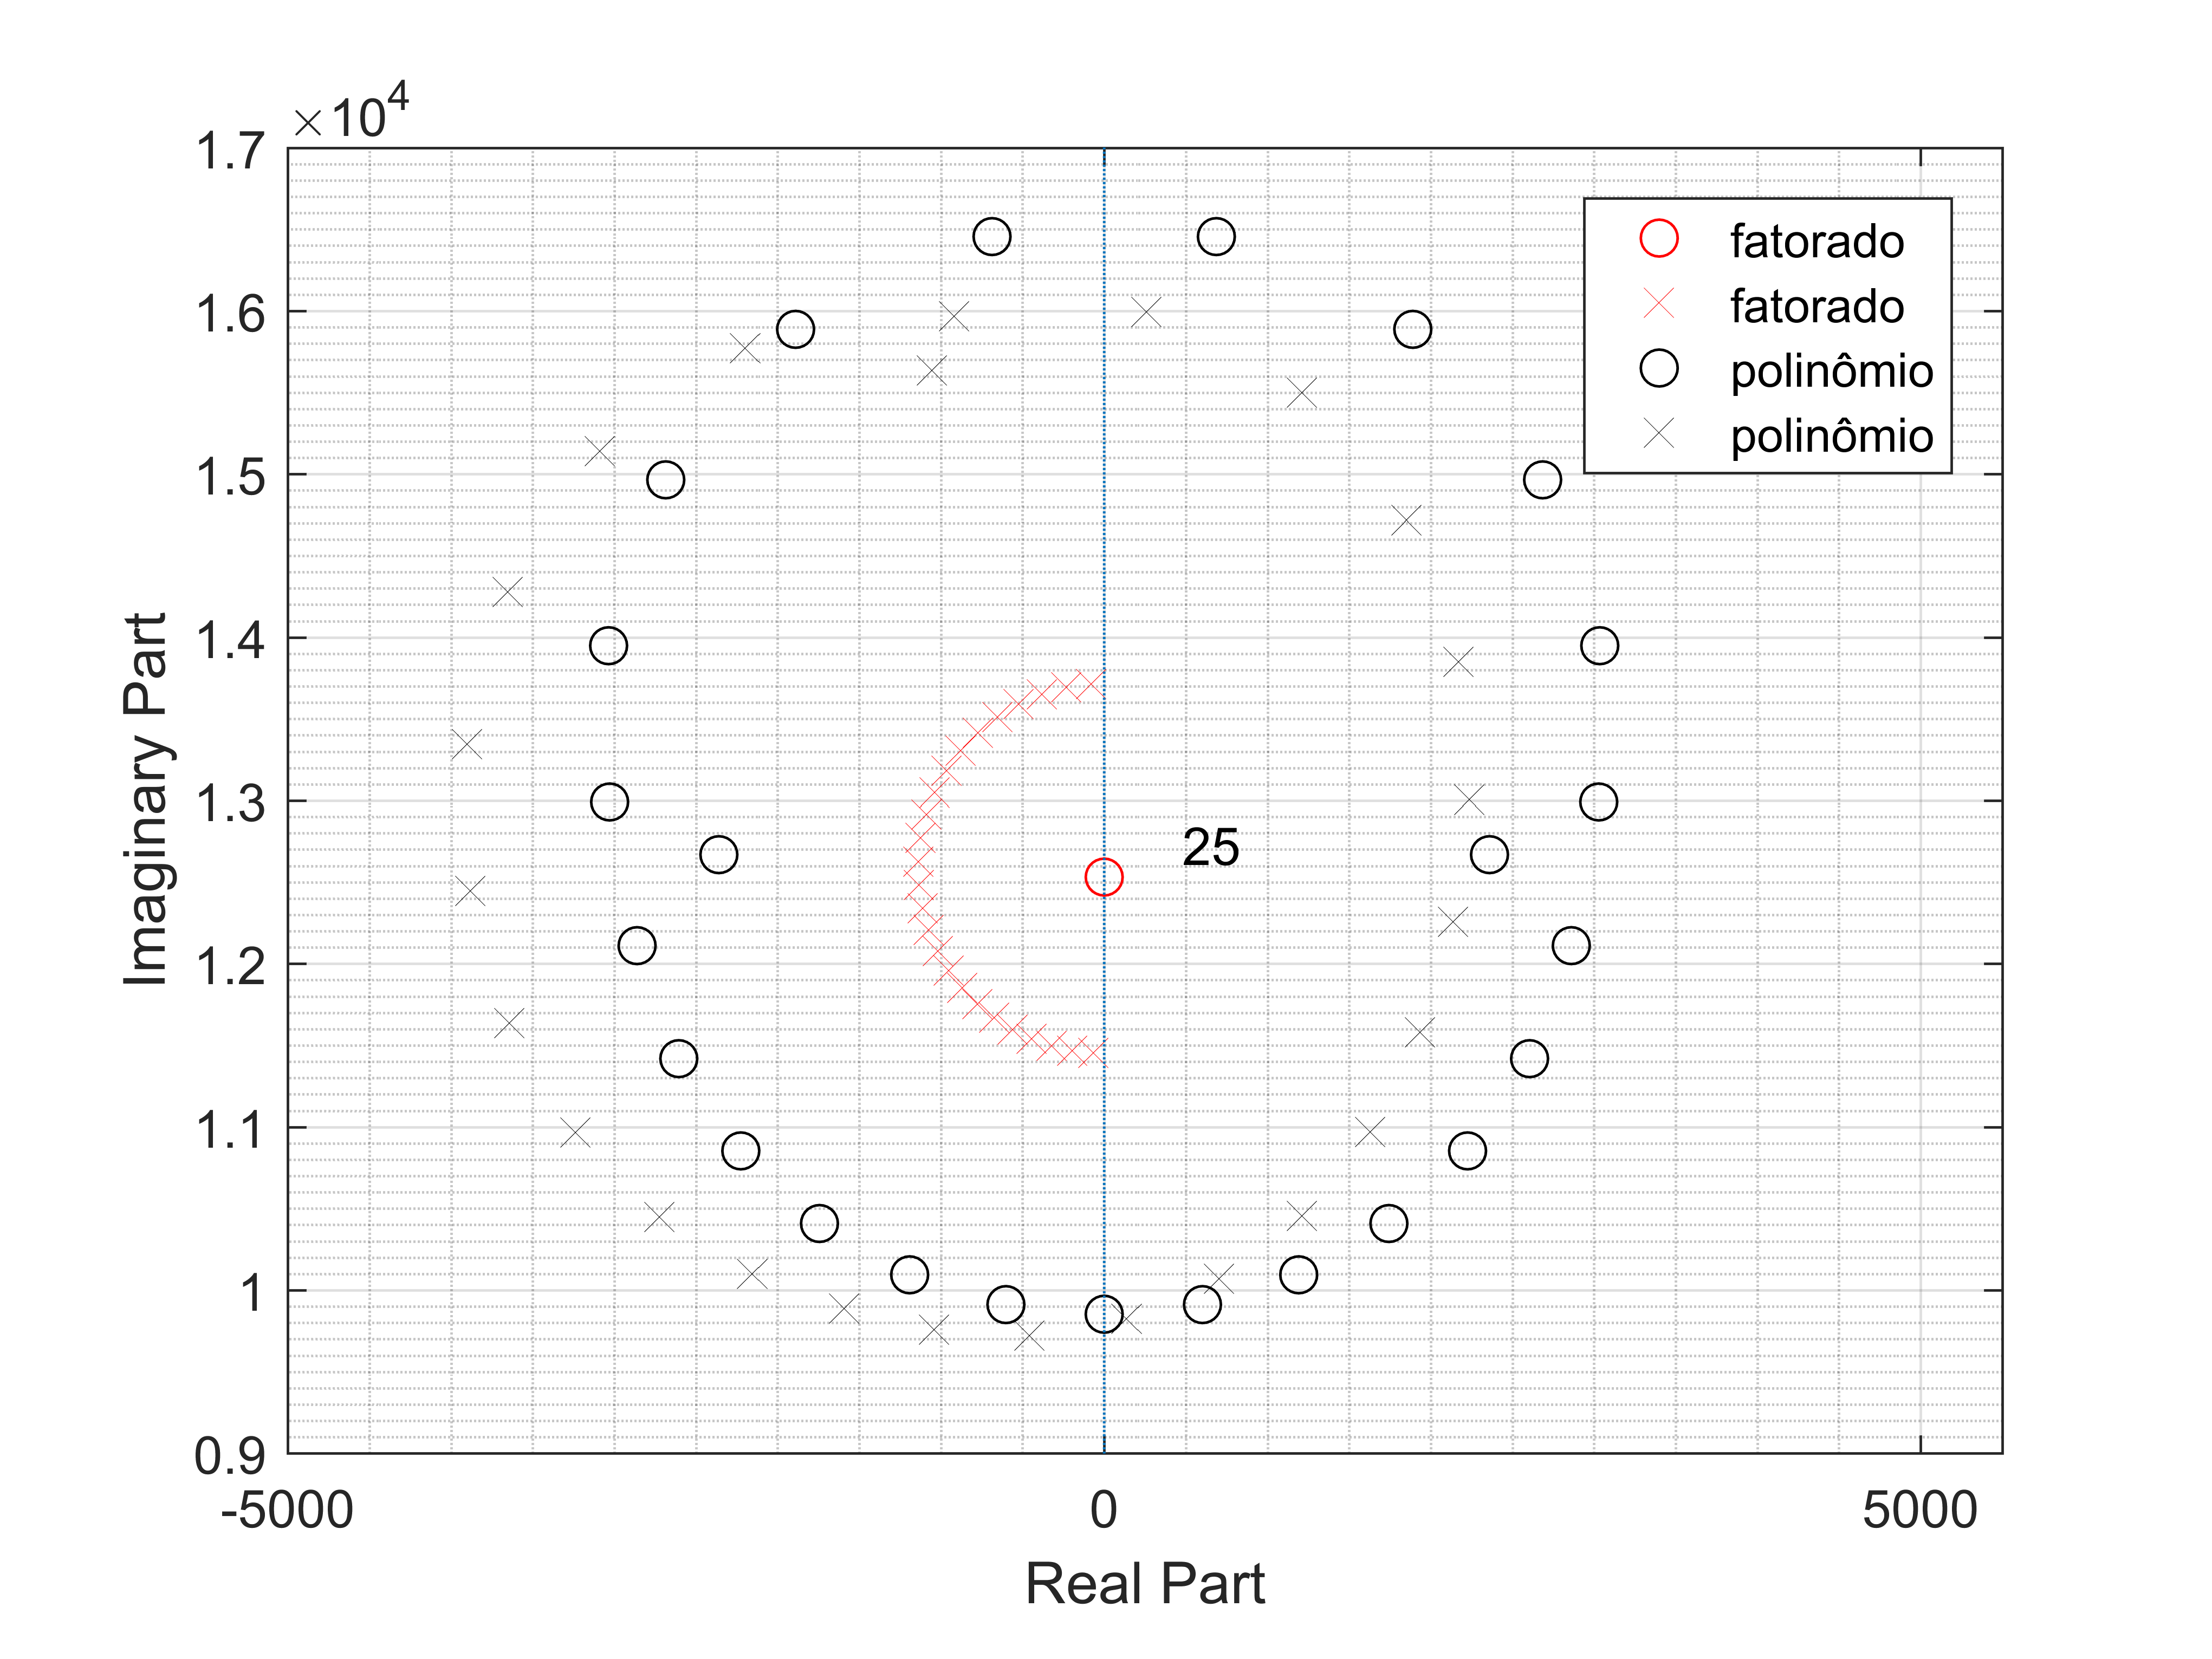
\includegraphics[width=0.6\textwidth]{graficos/z_plane_zpk_tf.PNG}
    \end{figure} 
    
\end{frame}

\begin{frame}{Tentativa 2 de cálculo de H(s)=N(s)/D(s)}
    Apenas para fins de análise o filtro instável foi discretizado e usado na filtragem do sinal. Como esperado, houve overflow com poucos milisegundos
        \begin{figure}[!htb]
    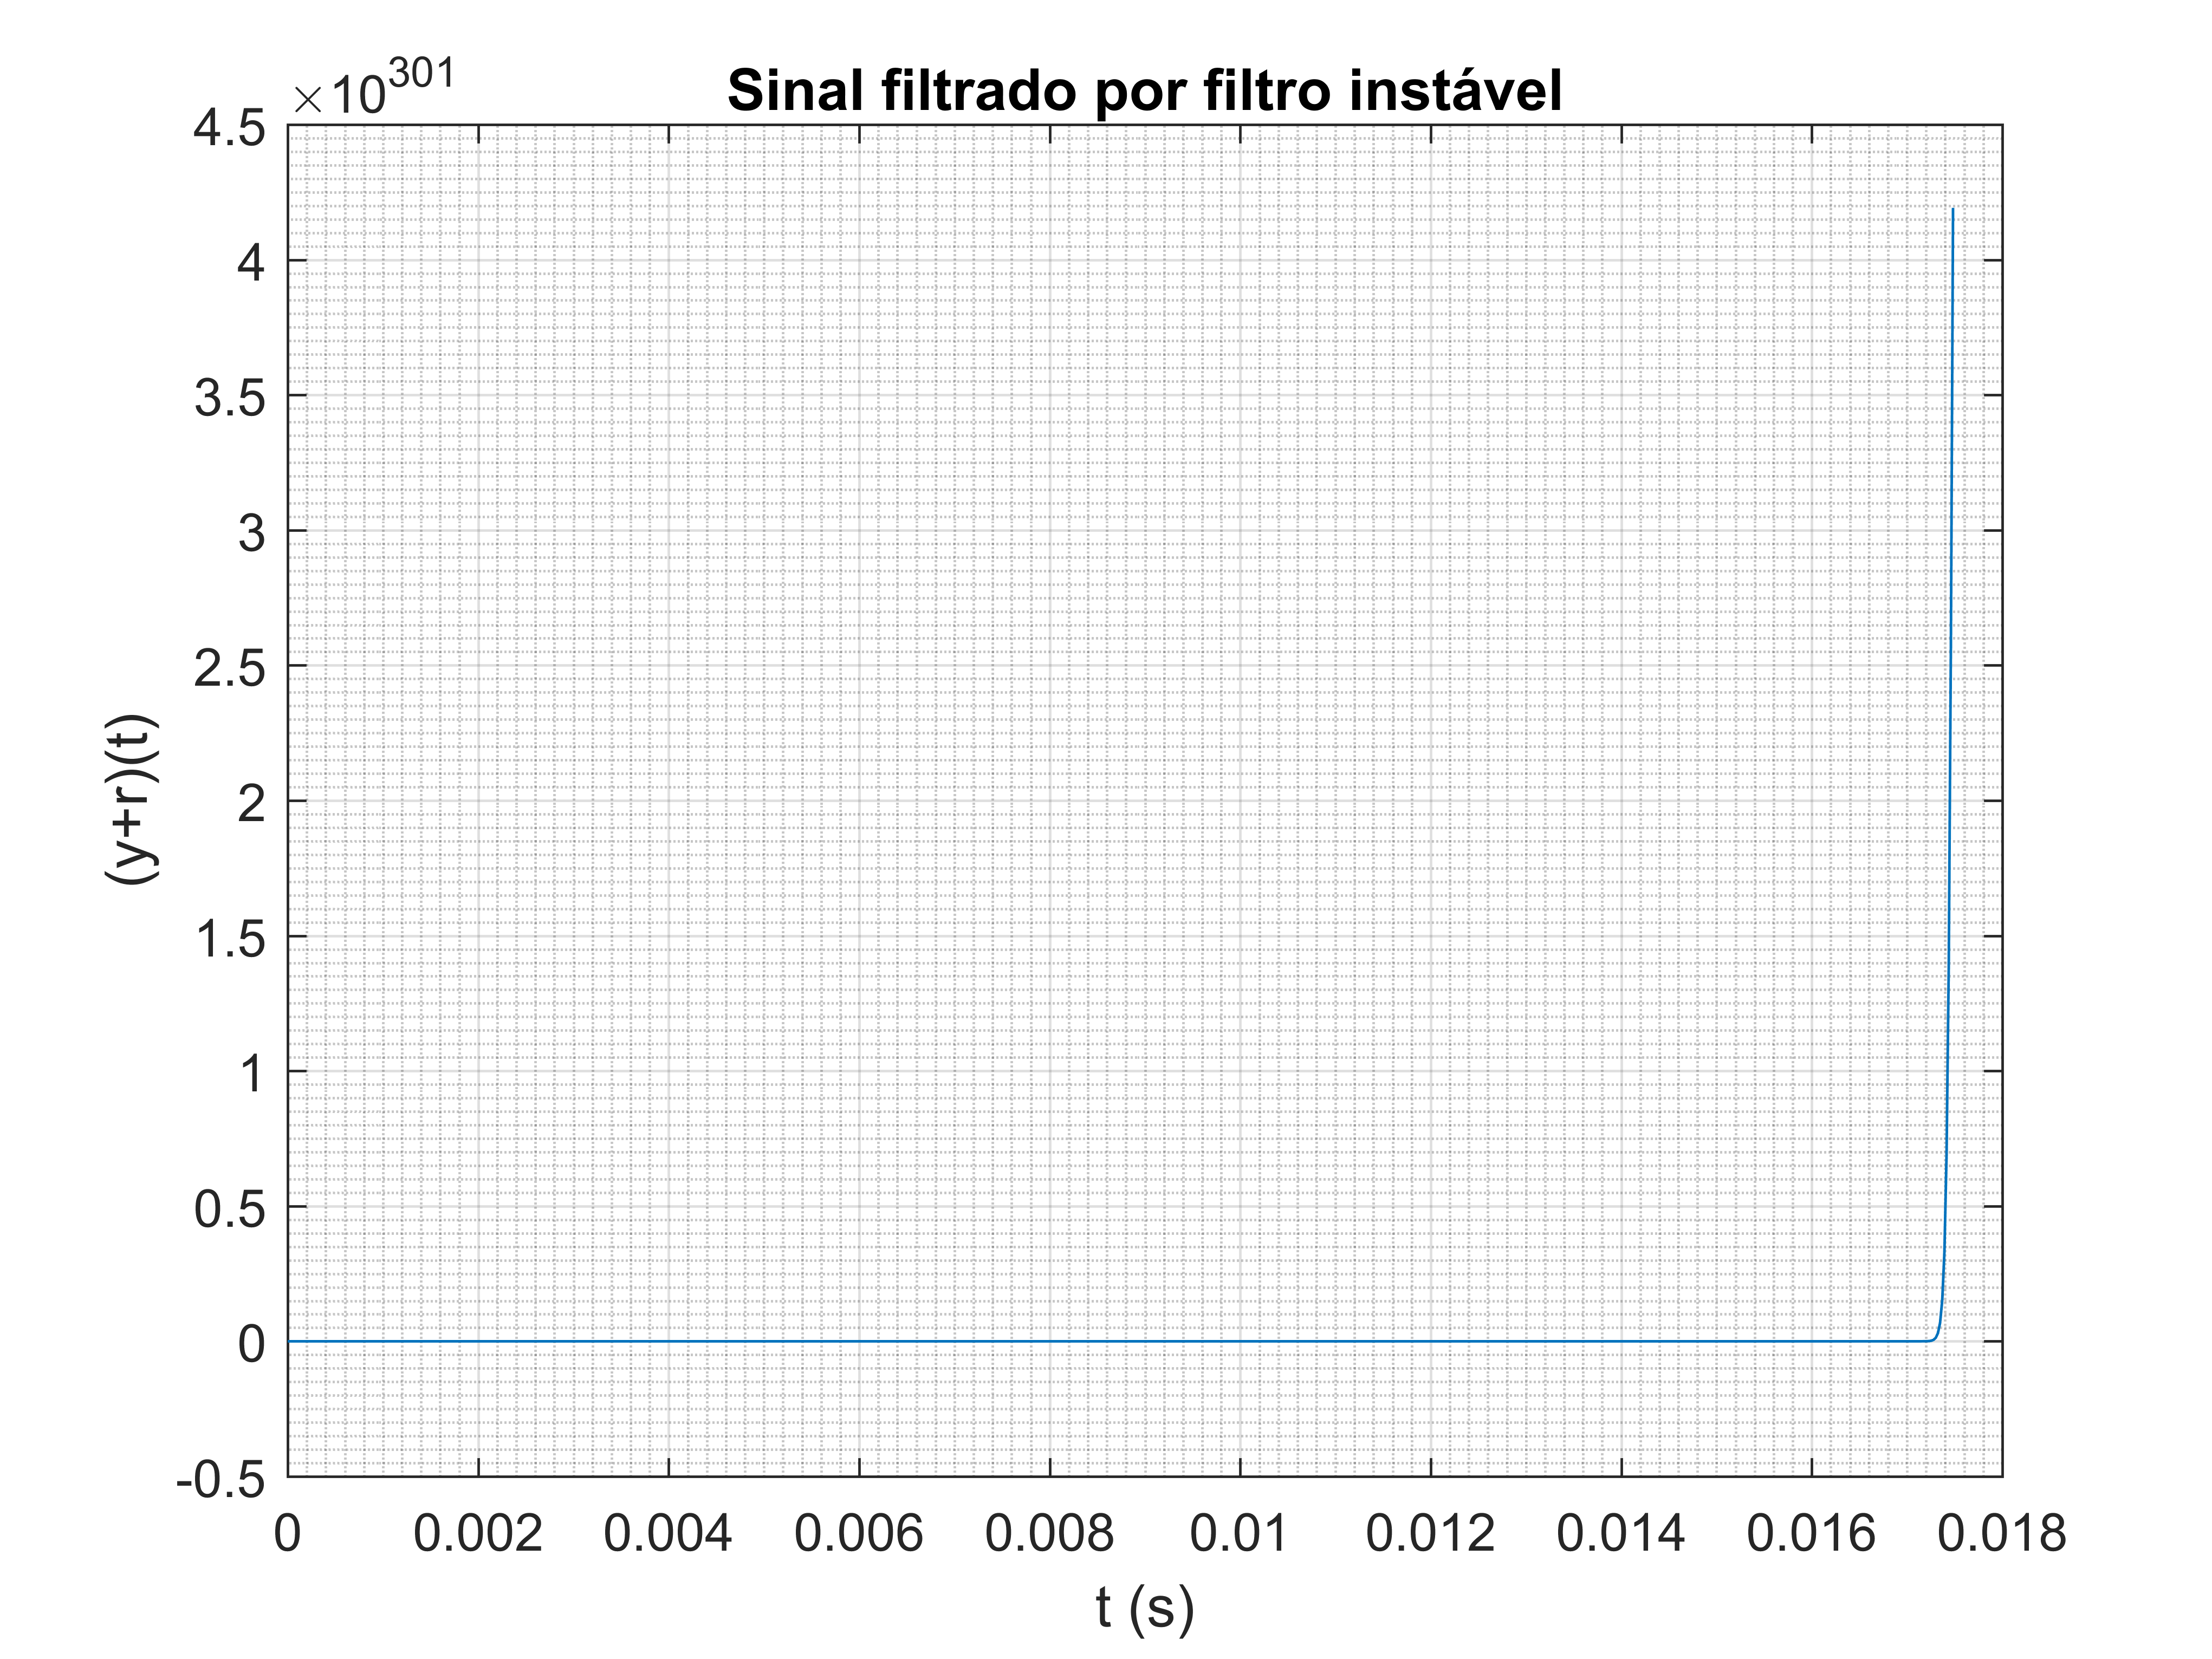
\includegraphics[width=0.6\textwidth]{graficos/filtro_instavel_t.PNG}
    \end{figure} 
    
\end{frame}

\begin{frame}{Tentativa 2 de cálculo de H(s)=N(s)/D(s)}
    Os pólos/zeros do SPD, após discretizados, ficaram fora do círculo unitário e a resposta em fase e magnitude teve comportamento totalmente diferente do desejado para um rejeita-faixa
    \begin{figure}[!htb]
    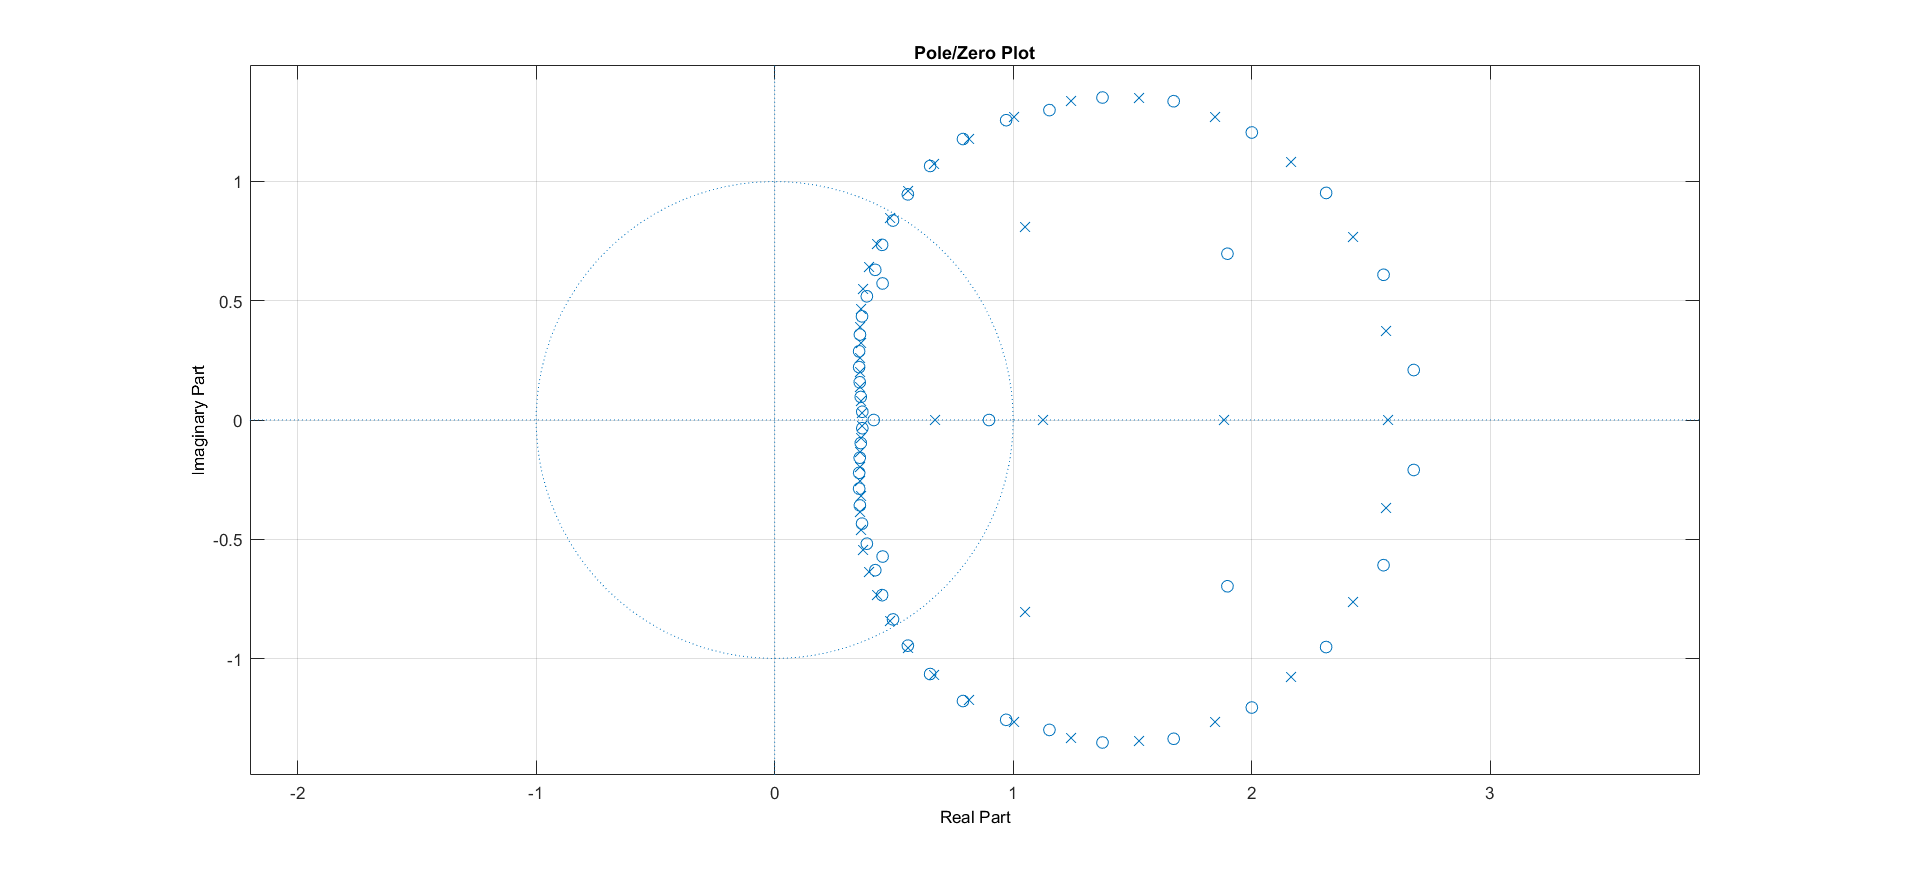
\includegraphics[width=0.9\textwidth]{graficos/zp_b_inst.PNG}
    \end{figure} 
\end{frame}
\begin{frame}{Tentativa 2 de cálculo de H(s)=N(s)/D(s)}
    \begin{figure}[!htb]
    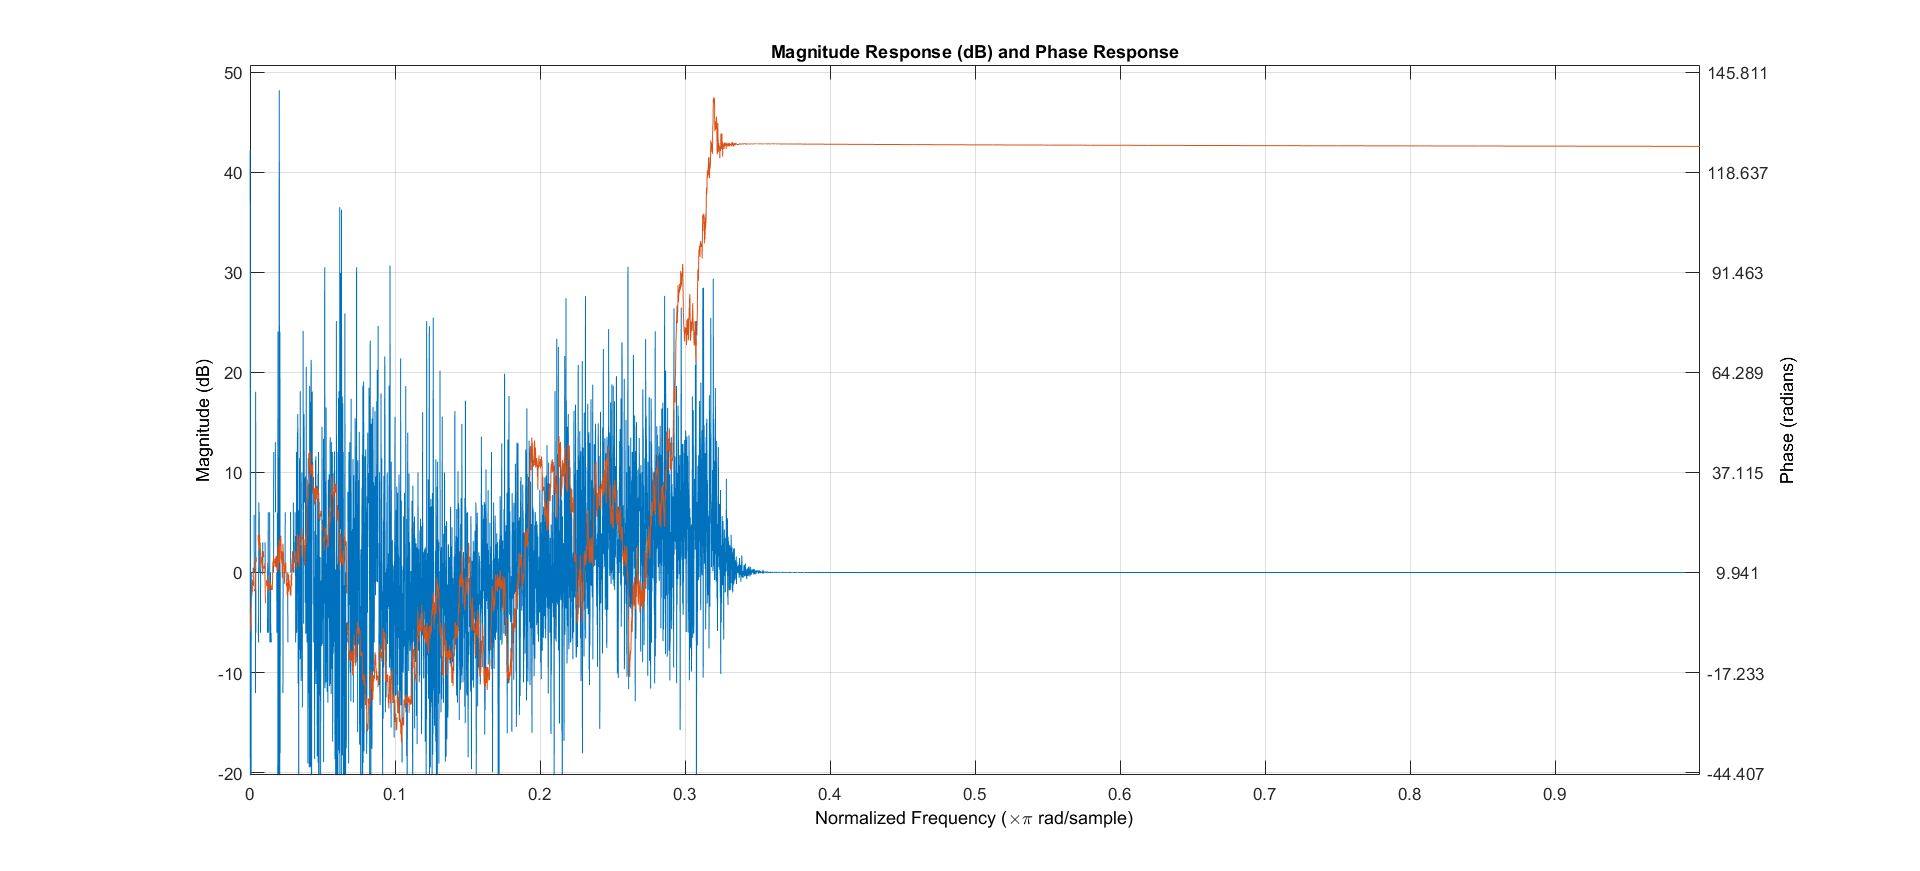
\includegraphics[width=0.9\textwidth]{graficos/mag_pha_b_inst.PNG}
    \end{figure} 
\end{frame}

\begin{frame}{Mitigação de Erro Numérico}
    \begin{itemize}
        \item Noutou-se que ordens altas de polinômios em funções de transferência são suceptíveis a erros númericos
        \item Polos/zeros podem deixar de ser estáveis/fase-mínima
        \item Contornou-se isto com cascatas de sistemas de segunda ordem
        \item O MATLAB usa as SOS (second order sections)
        \item sosfilt(SOS,X) é análoga ao filt(NUM,DEN,Ts) para SOS
    \end{itemize}

\end{frame}

\begin{frame}{Mitigação de Erro Numérico}
    \begin{figure}[!htb]
    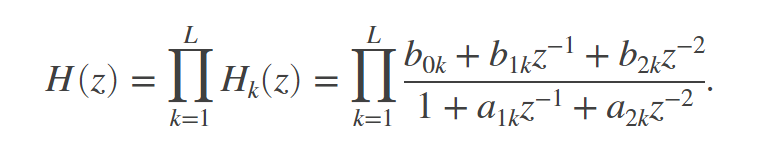
\includegraphics[width=0.6\textwidth]{graficos/eq_sos.PNG}
    \end{figure} 
	\begin{figure}[!htb]
    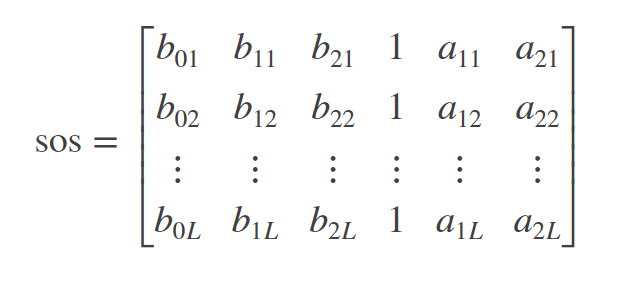
\includegraphics[width=0.6\textwidth]{graficos/matriz_sos.PNG}
    \end{figure} 
\end{frame}

\begin{frame}{Mitigação de Erro Numérico}
    \begin{figure}[!htb]
    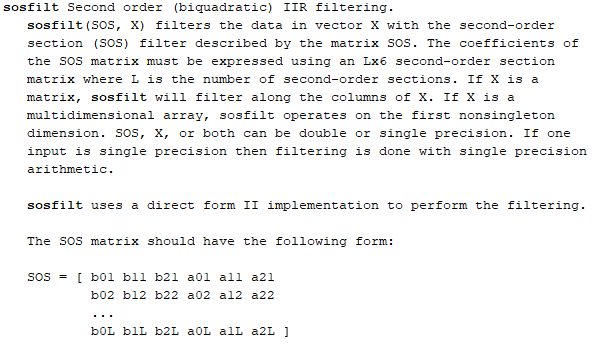
\includegraphics[width=0.9\textwidth]{graficos/sos_filt_doc.png}
    \end{figure}
    
\end{frame}

\begin{frame}{Butterworth e Chebyshev I}
    \begin{figure}[!htb]
    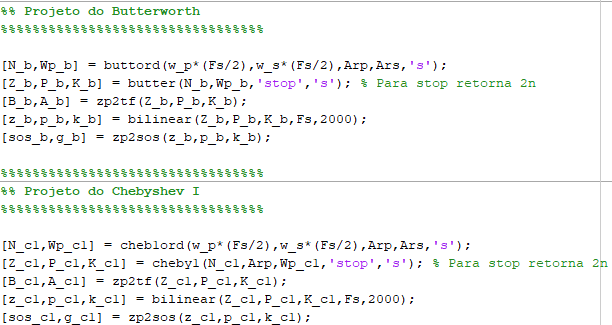
\includegraphics[width=0.9\textwidth]{graficos/code_butt_chebI.PNG}
    \end{figure} 
\end{frame}


\begin{frame}{Chebyshev II e Elíptico}
    \begin{figure}[!htb]
    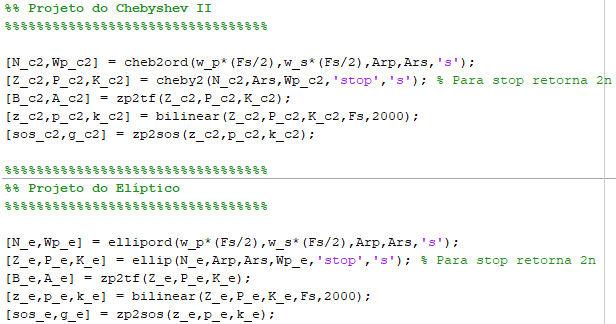
\includegraphics[width=0.9\textwidth]{graficos/code_chebII_ellip.png}
    \end{figure} 
\end{frame}


\begin{frame}{Filtragem das SOS calculadas}
    \begin{figure}[!htb]
    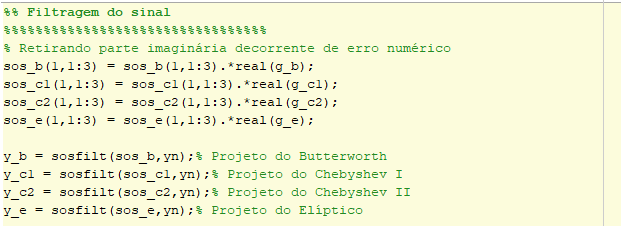
\includegraphics[width=0.9\textwidth]{graficos/code_sos_filtros.png}
    \end{figure} 
\end{frame}

% Resultados
\section{Resultados}
\begin{frame}{Resposta em Magnitude e Fase - Butterworth}
    \begin{figure}
        \centering
        \includegraphics[width=1.1\textwidth]{graficos/mag_pha_b.png}
    \end{figure}
\end{frame}

\begin{frame}{Pólos e Zeros - Butterworth}
    \begin{figure}
        \centering
        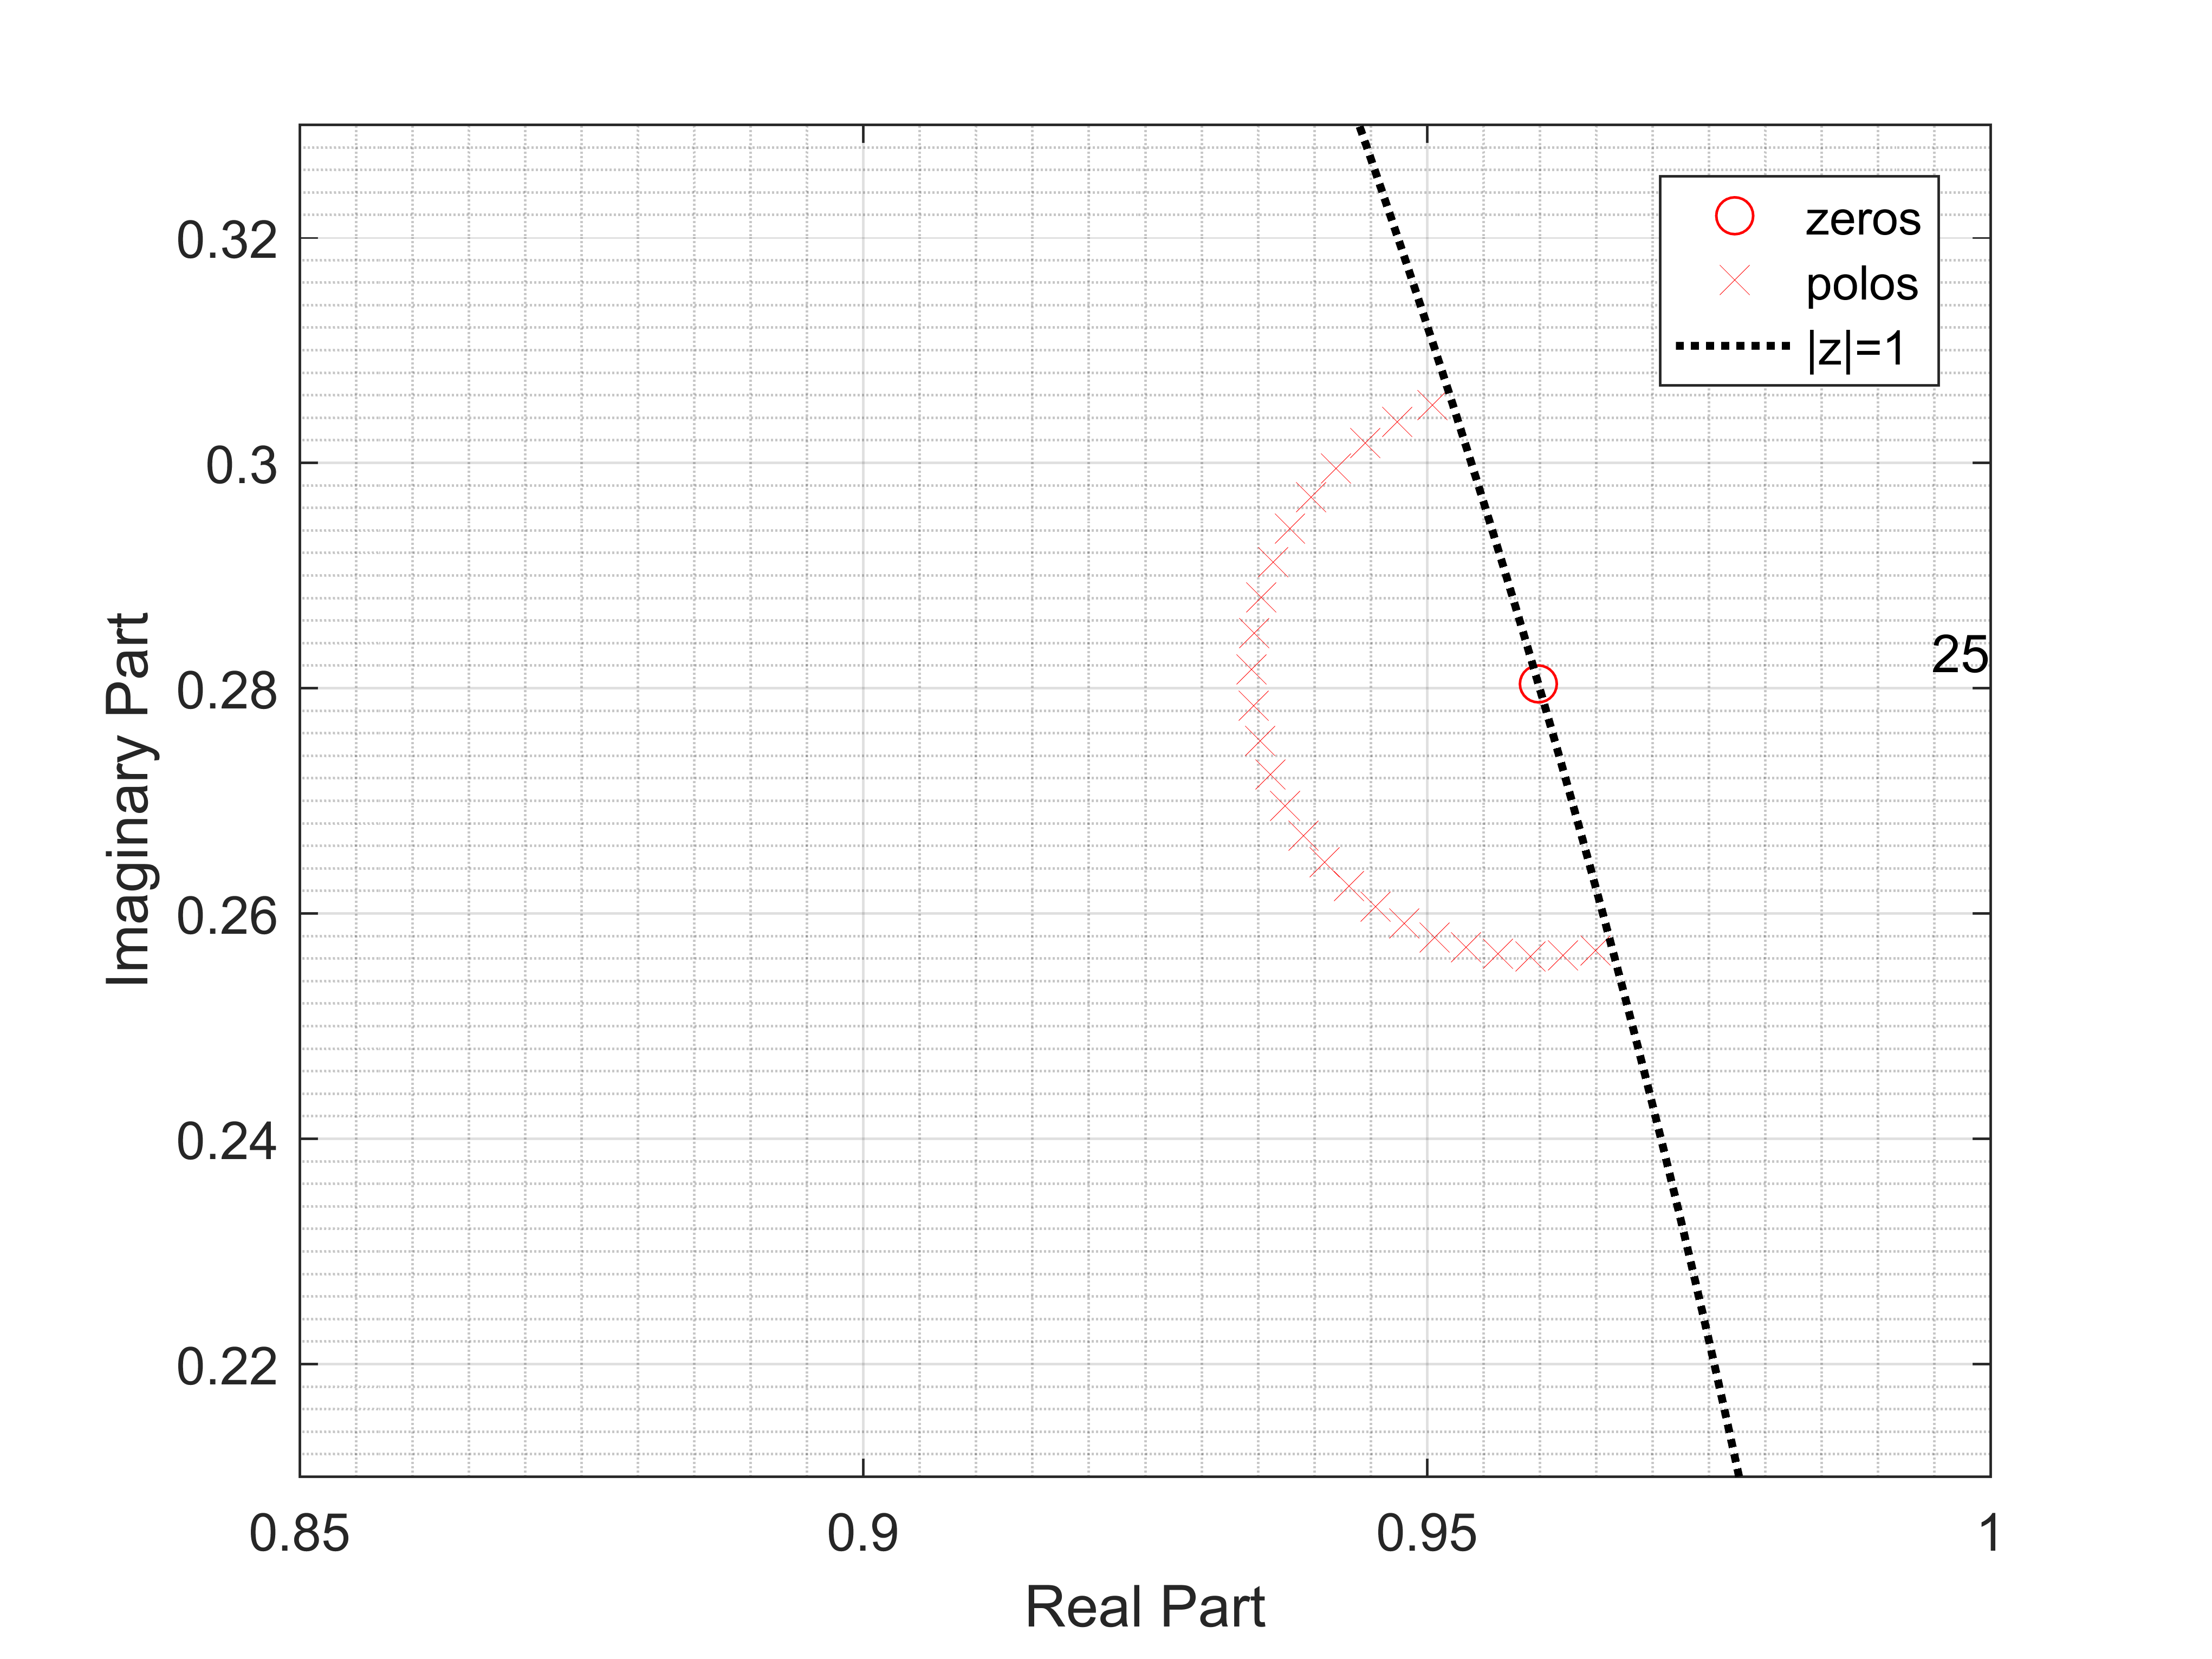
\includegraphics[width=0.7\textwidth]{graficos/zp_b.png}
    \end{figure}
\end{frame}

\begin{frame}{Resposta em Magnitude e Fase - Chebyshev I}
    \begin{figure}
        \centering
        \includegraphics[width=1.1\textwidth]{graficos/mag_pha_c1.png}
    \end{figure}
\end{frame}

\begin{frame}{Pólos e Zeros - Chebyshev I}
    \begin{figure}
        \centering
        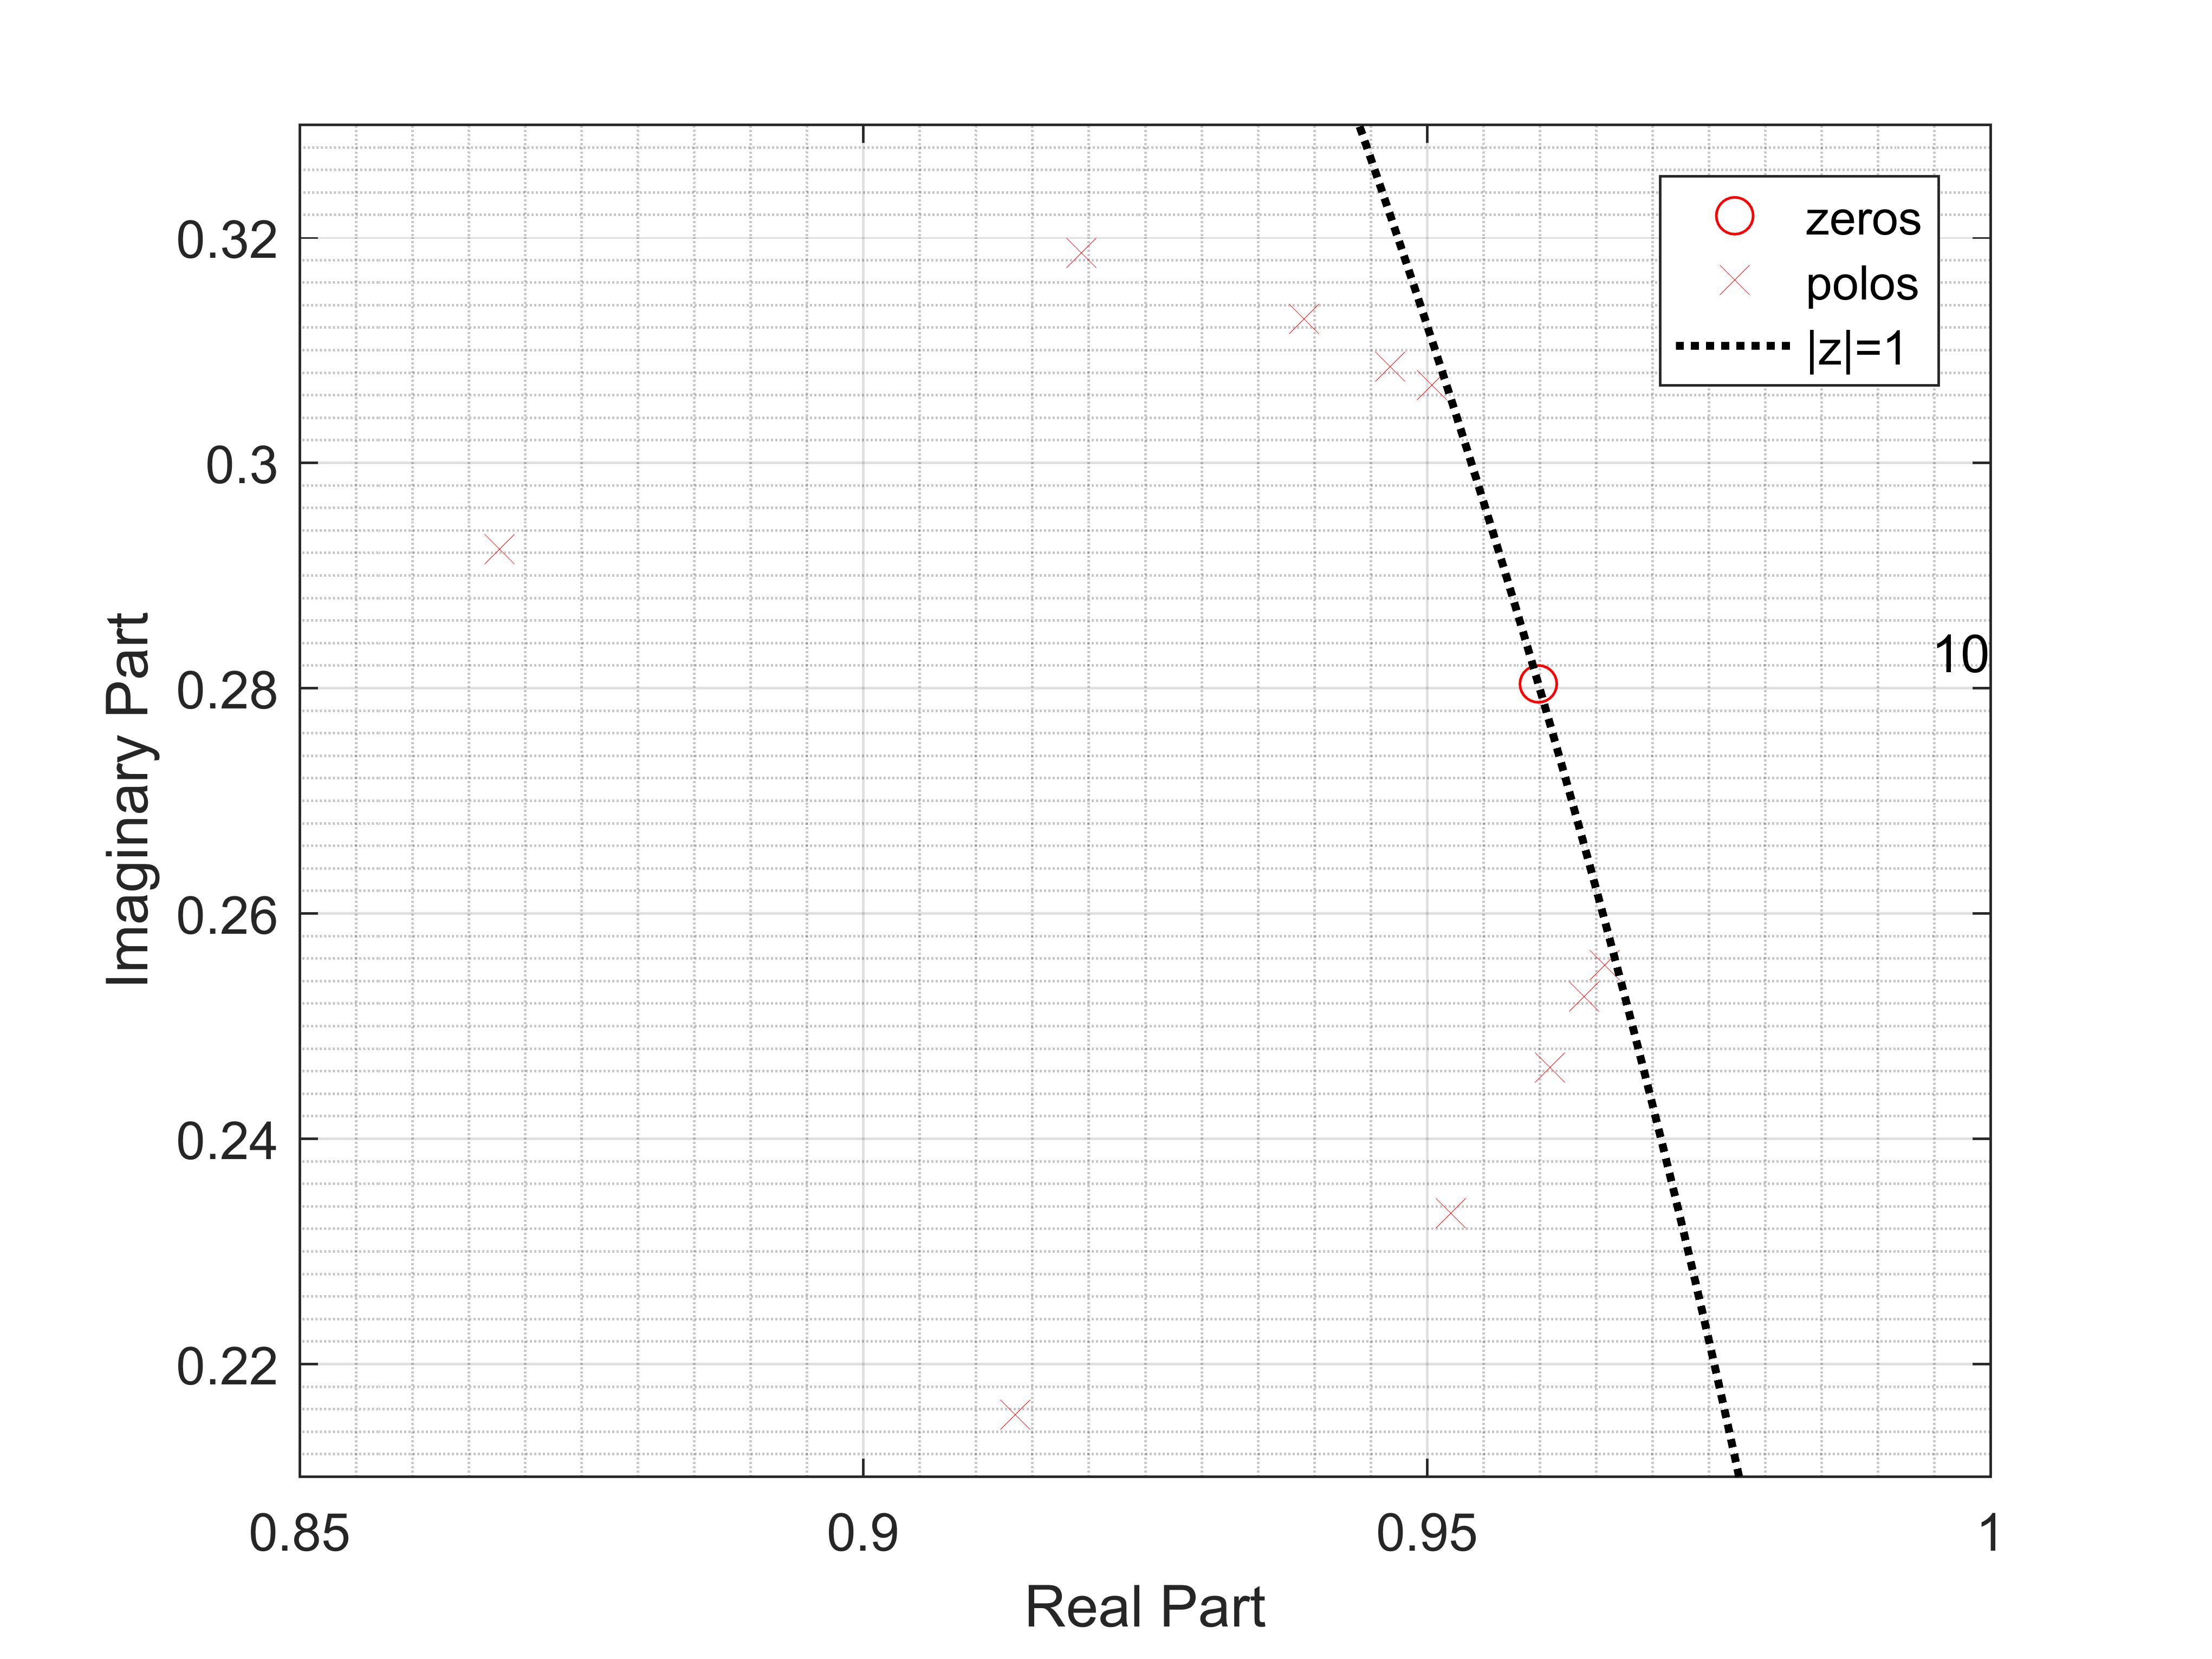
\includegraphics[width=0.7\textwidth]{graficos/zp_c1.png}
    \end{figure}
\end{frame}

\begin{frame}{Resposta em Magnitude e Fase - Chebyshev II}
    \begin{figure}
        \centering
        \includegraphics[width=1.1\textwidth]{graficos/mag_pha_c2.png}
    \end{figure}
\end{frame}

\begin{frame}{Pólos e Zeros - Chebyshev II}
    \begin{figure}
        \centering
        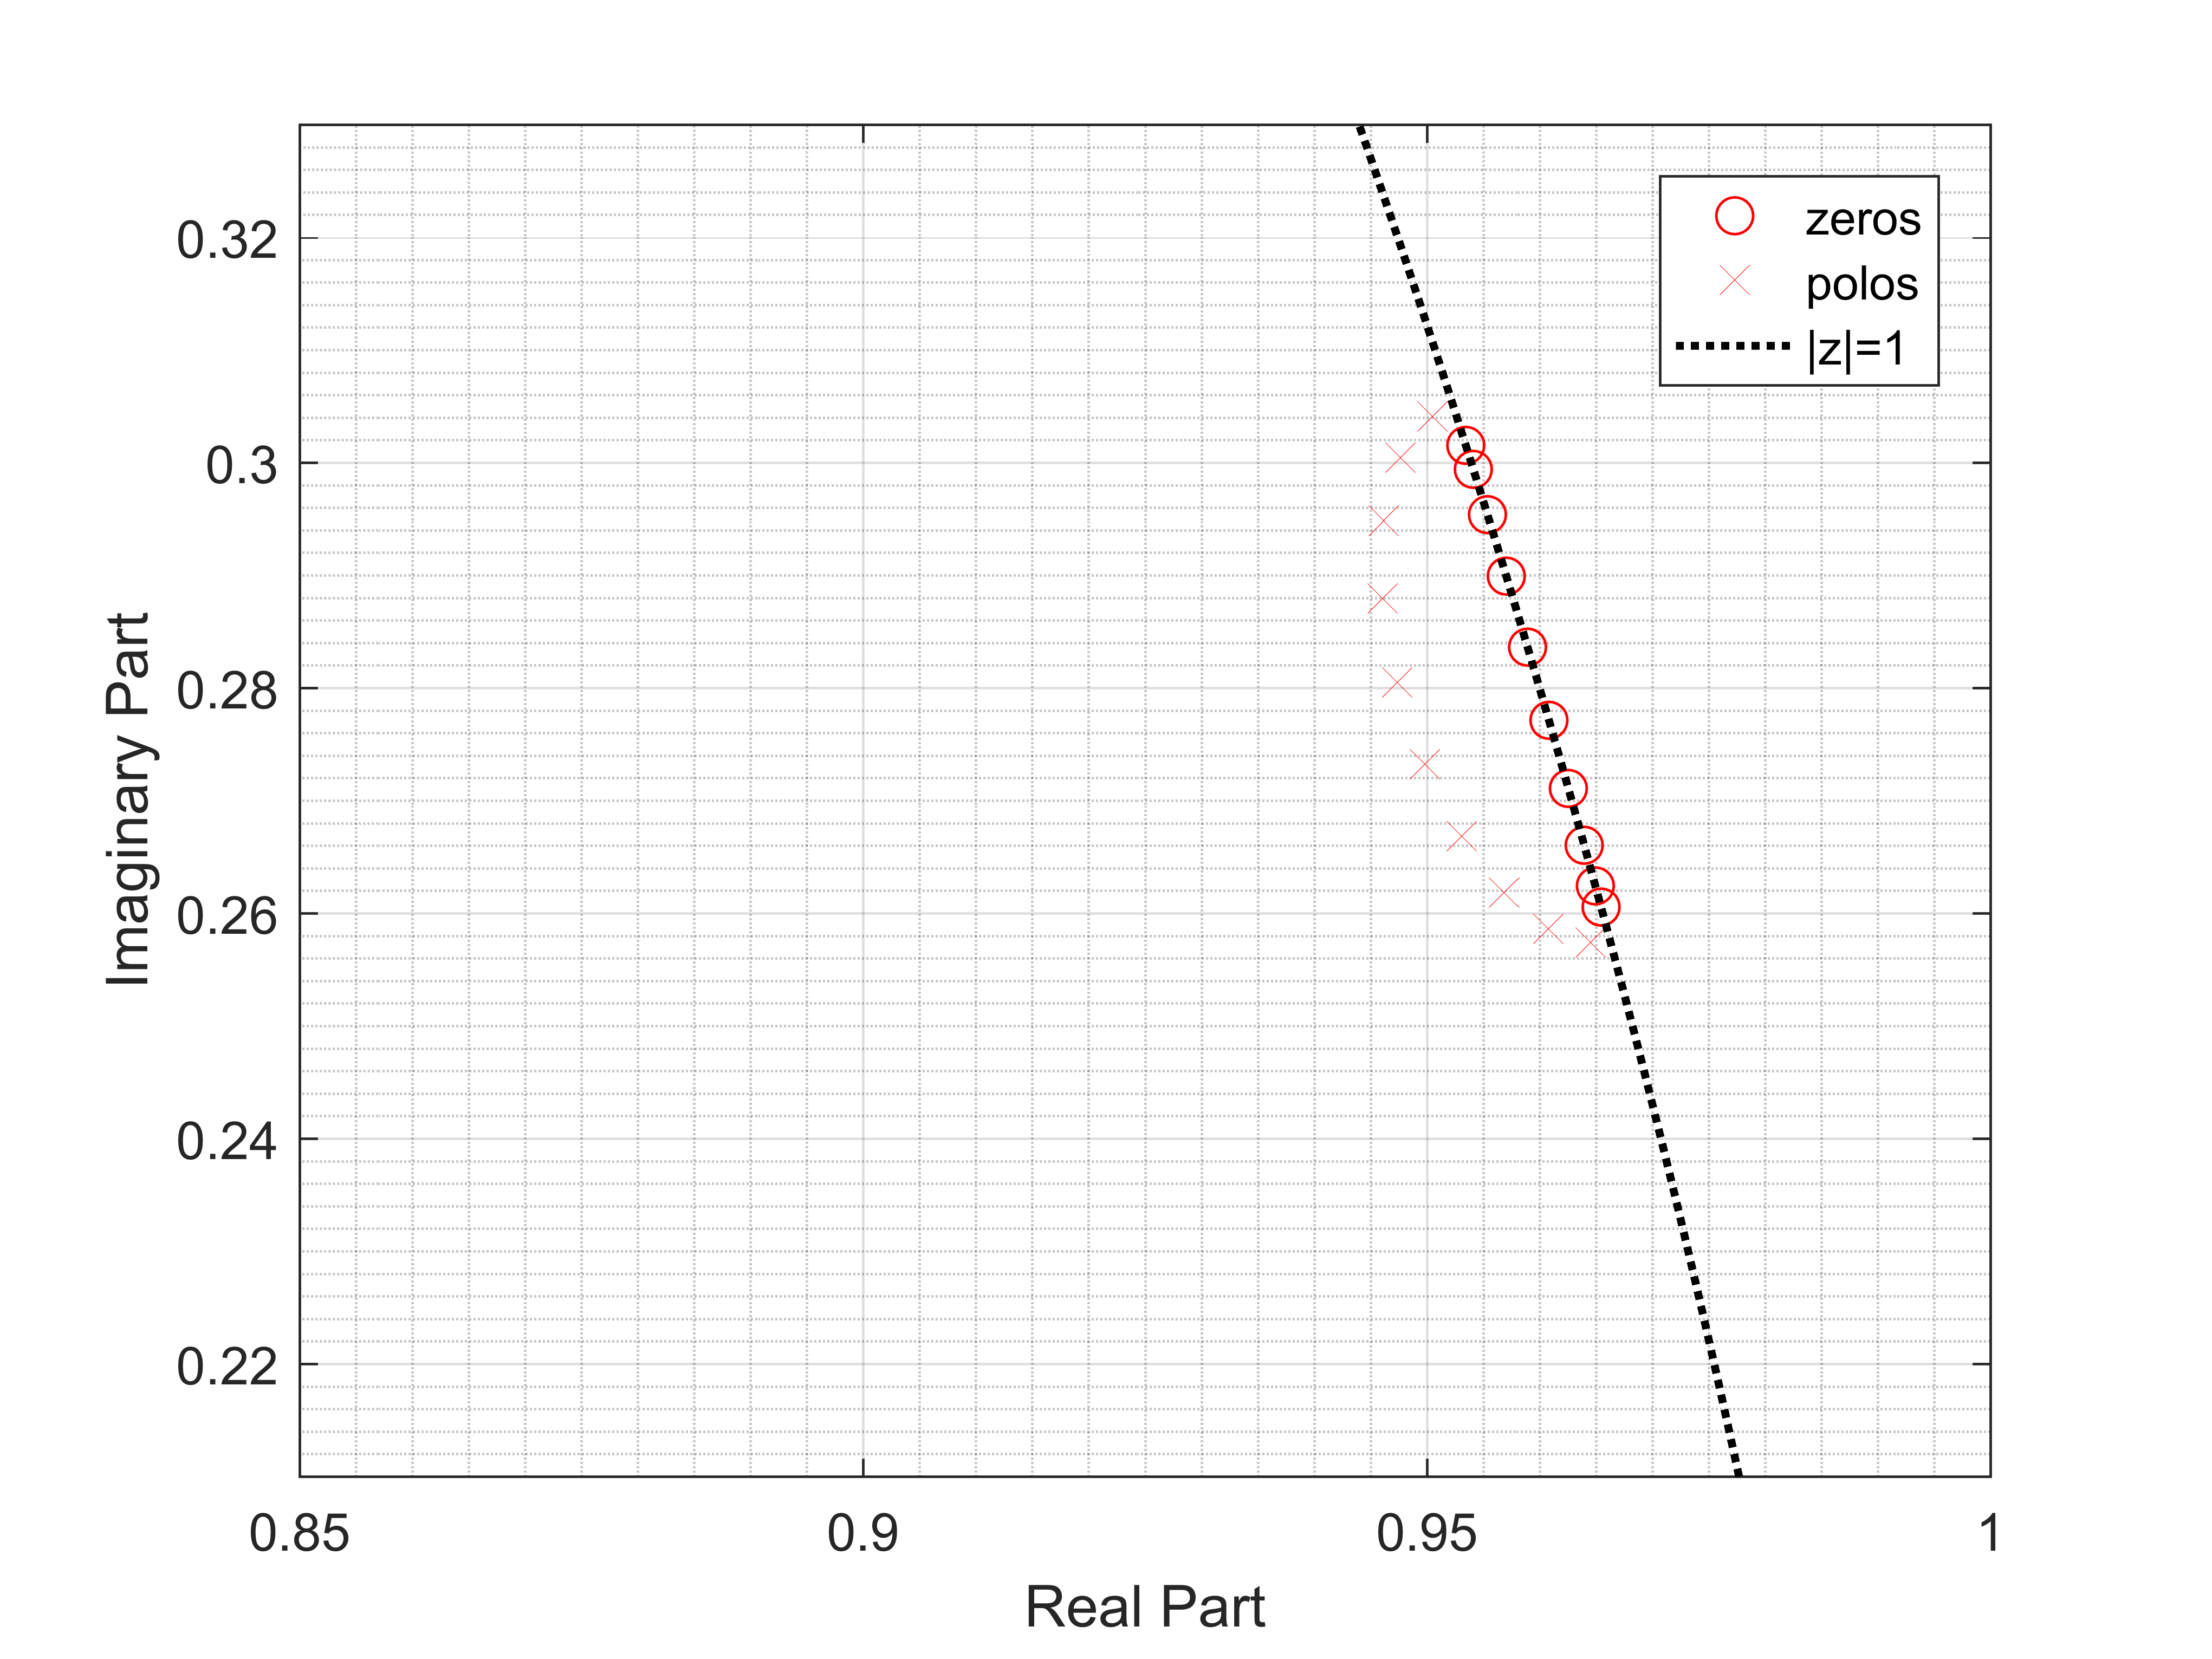
\includegraphics[width=0.7\textwidth]{graficos/zp_c2.png}
    \end{figure}
\end{frame}

\begin{frame}{Resposta em Magnitude e Fase - Elíptico}
    \begin{figure}
        \centering
        \includegraphics[width=1.1\textwidth]{graficos/mag_pha_e.png}
    \end{figure}
\end{frame}

\begin{frame}{Pólos e Zeros - Elíptico}
    \begin{figure}
        \centering
        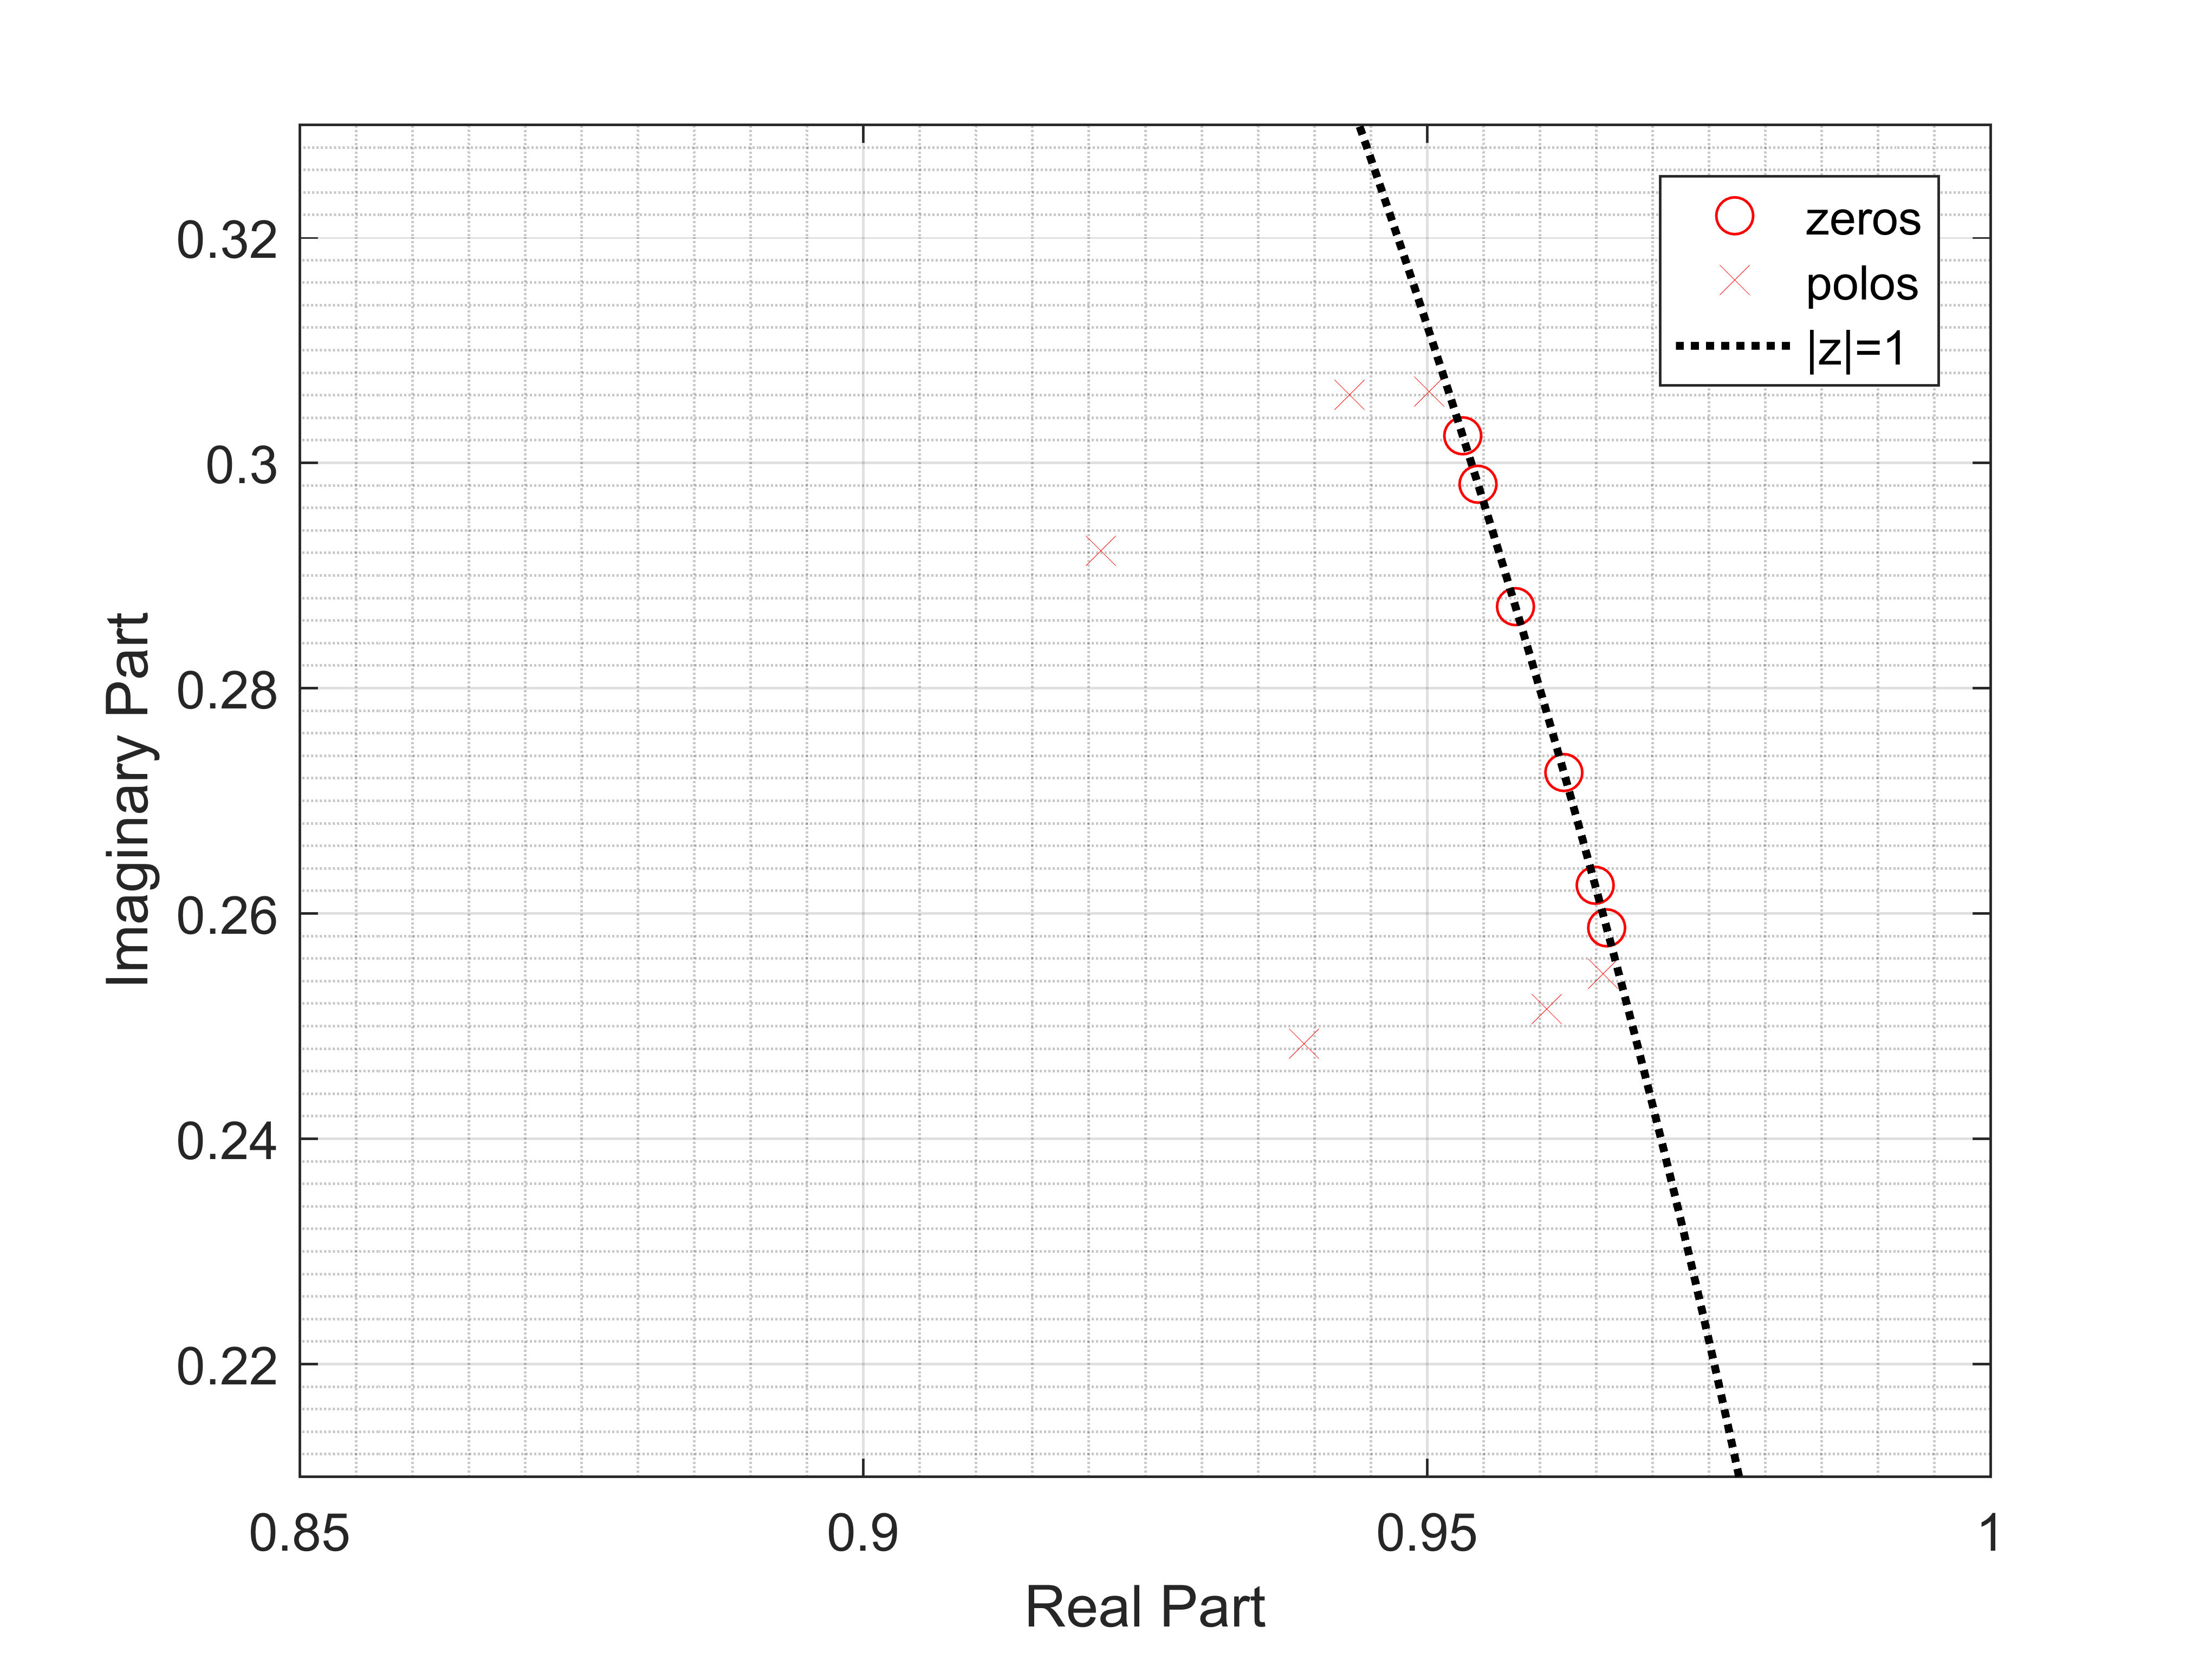
\includegraphics[width=0.7\textwidth]{graficos/zp_e.png}
    \end{figure}
\end{frame}

\begin{frame}{Sinais no tempo - Butterworth}
    \begin{figure}
        \centering
        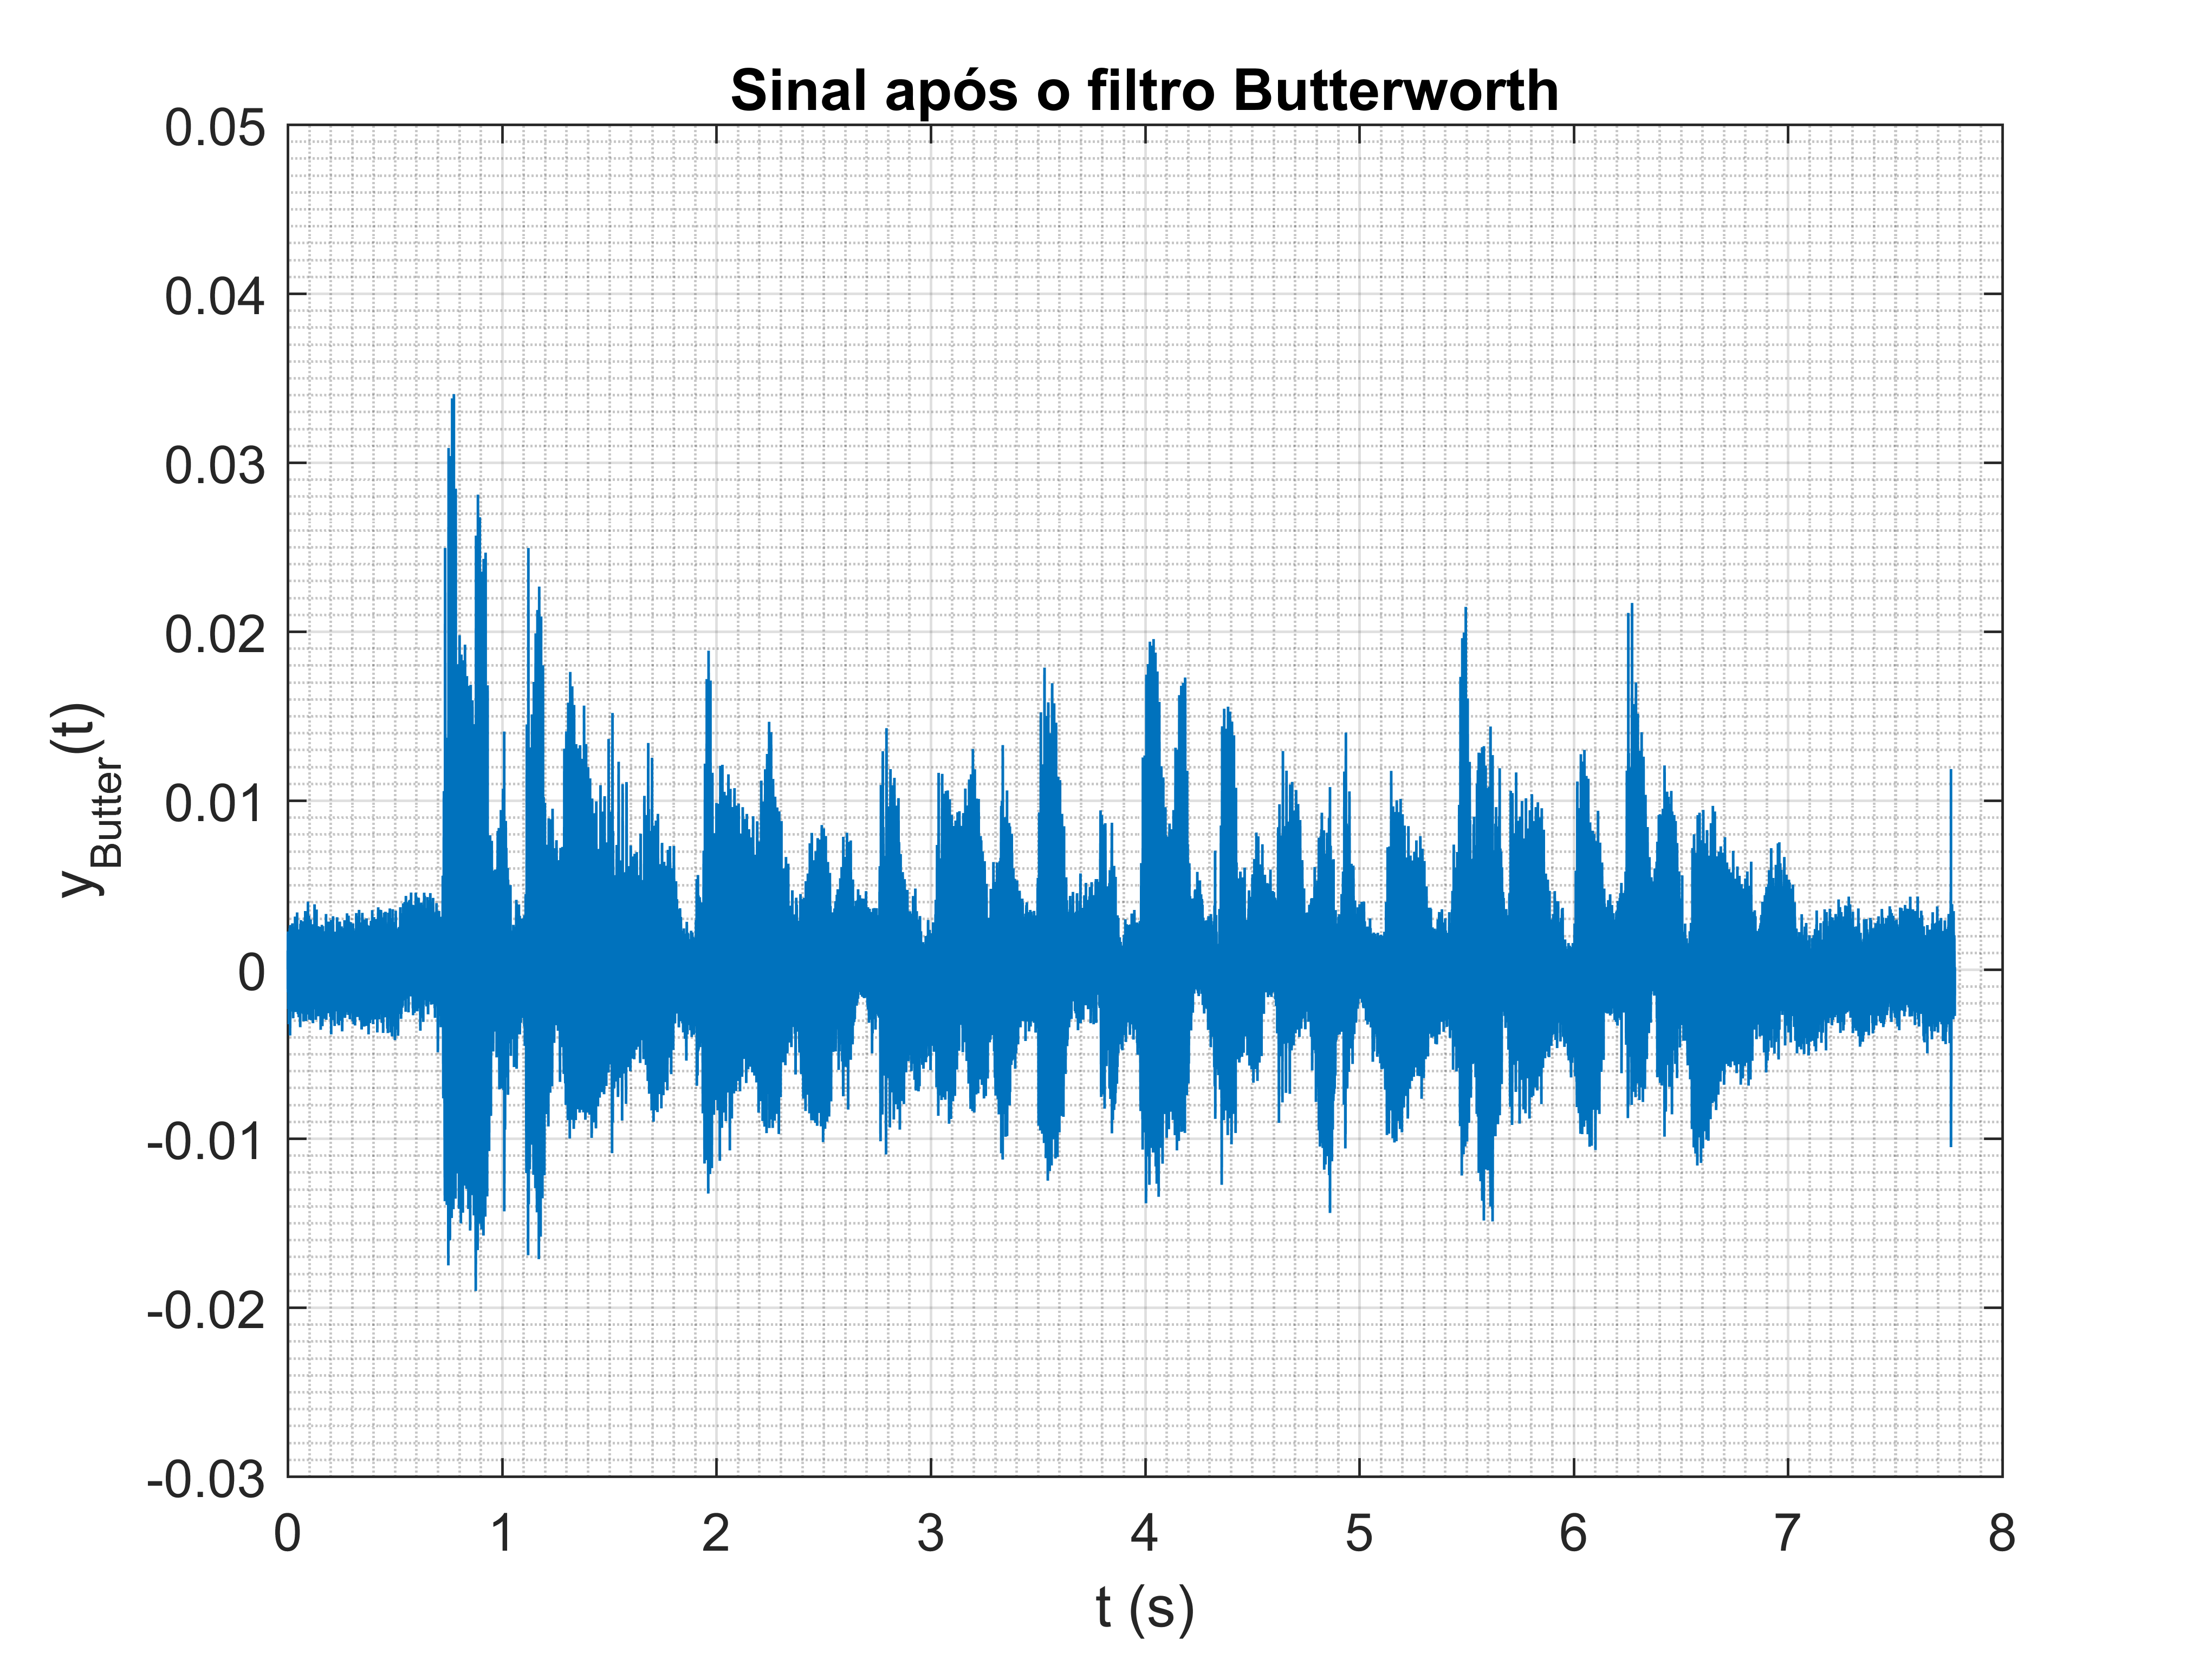
\includegraphics[width=0.7\textwidth]{graficos/filtrados_t_b.png}
    \end{figure}
\end{frame}
\begin{frame}{Sinais no tempo - Chebyshev I}
    \begin{figure}
        \centering
        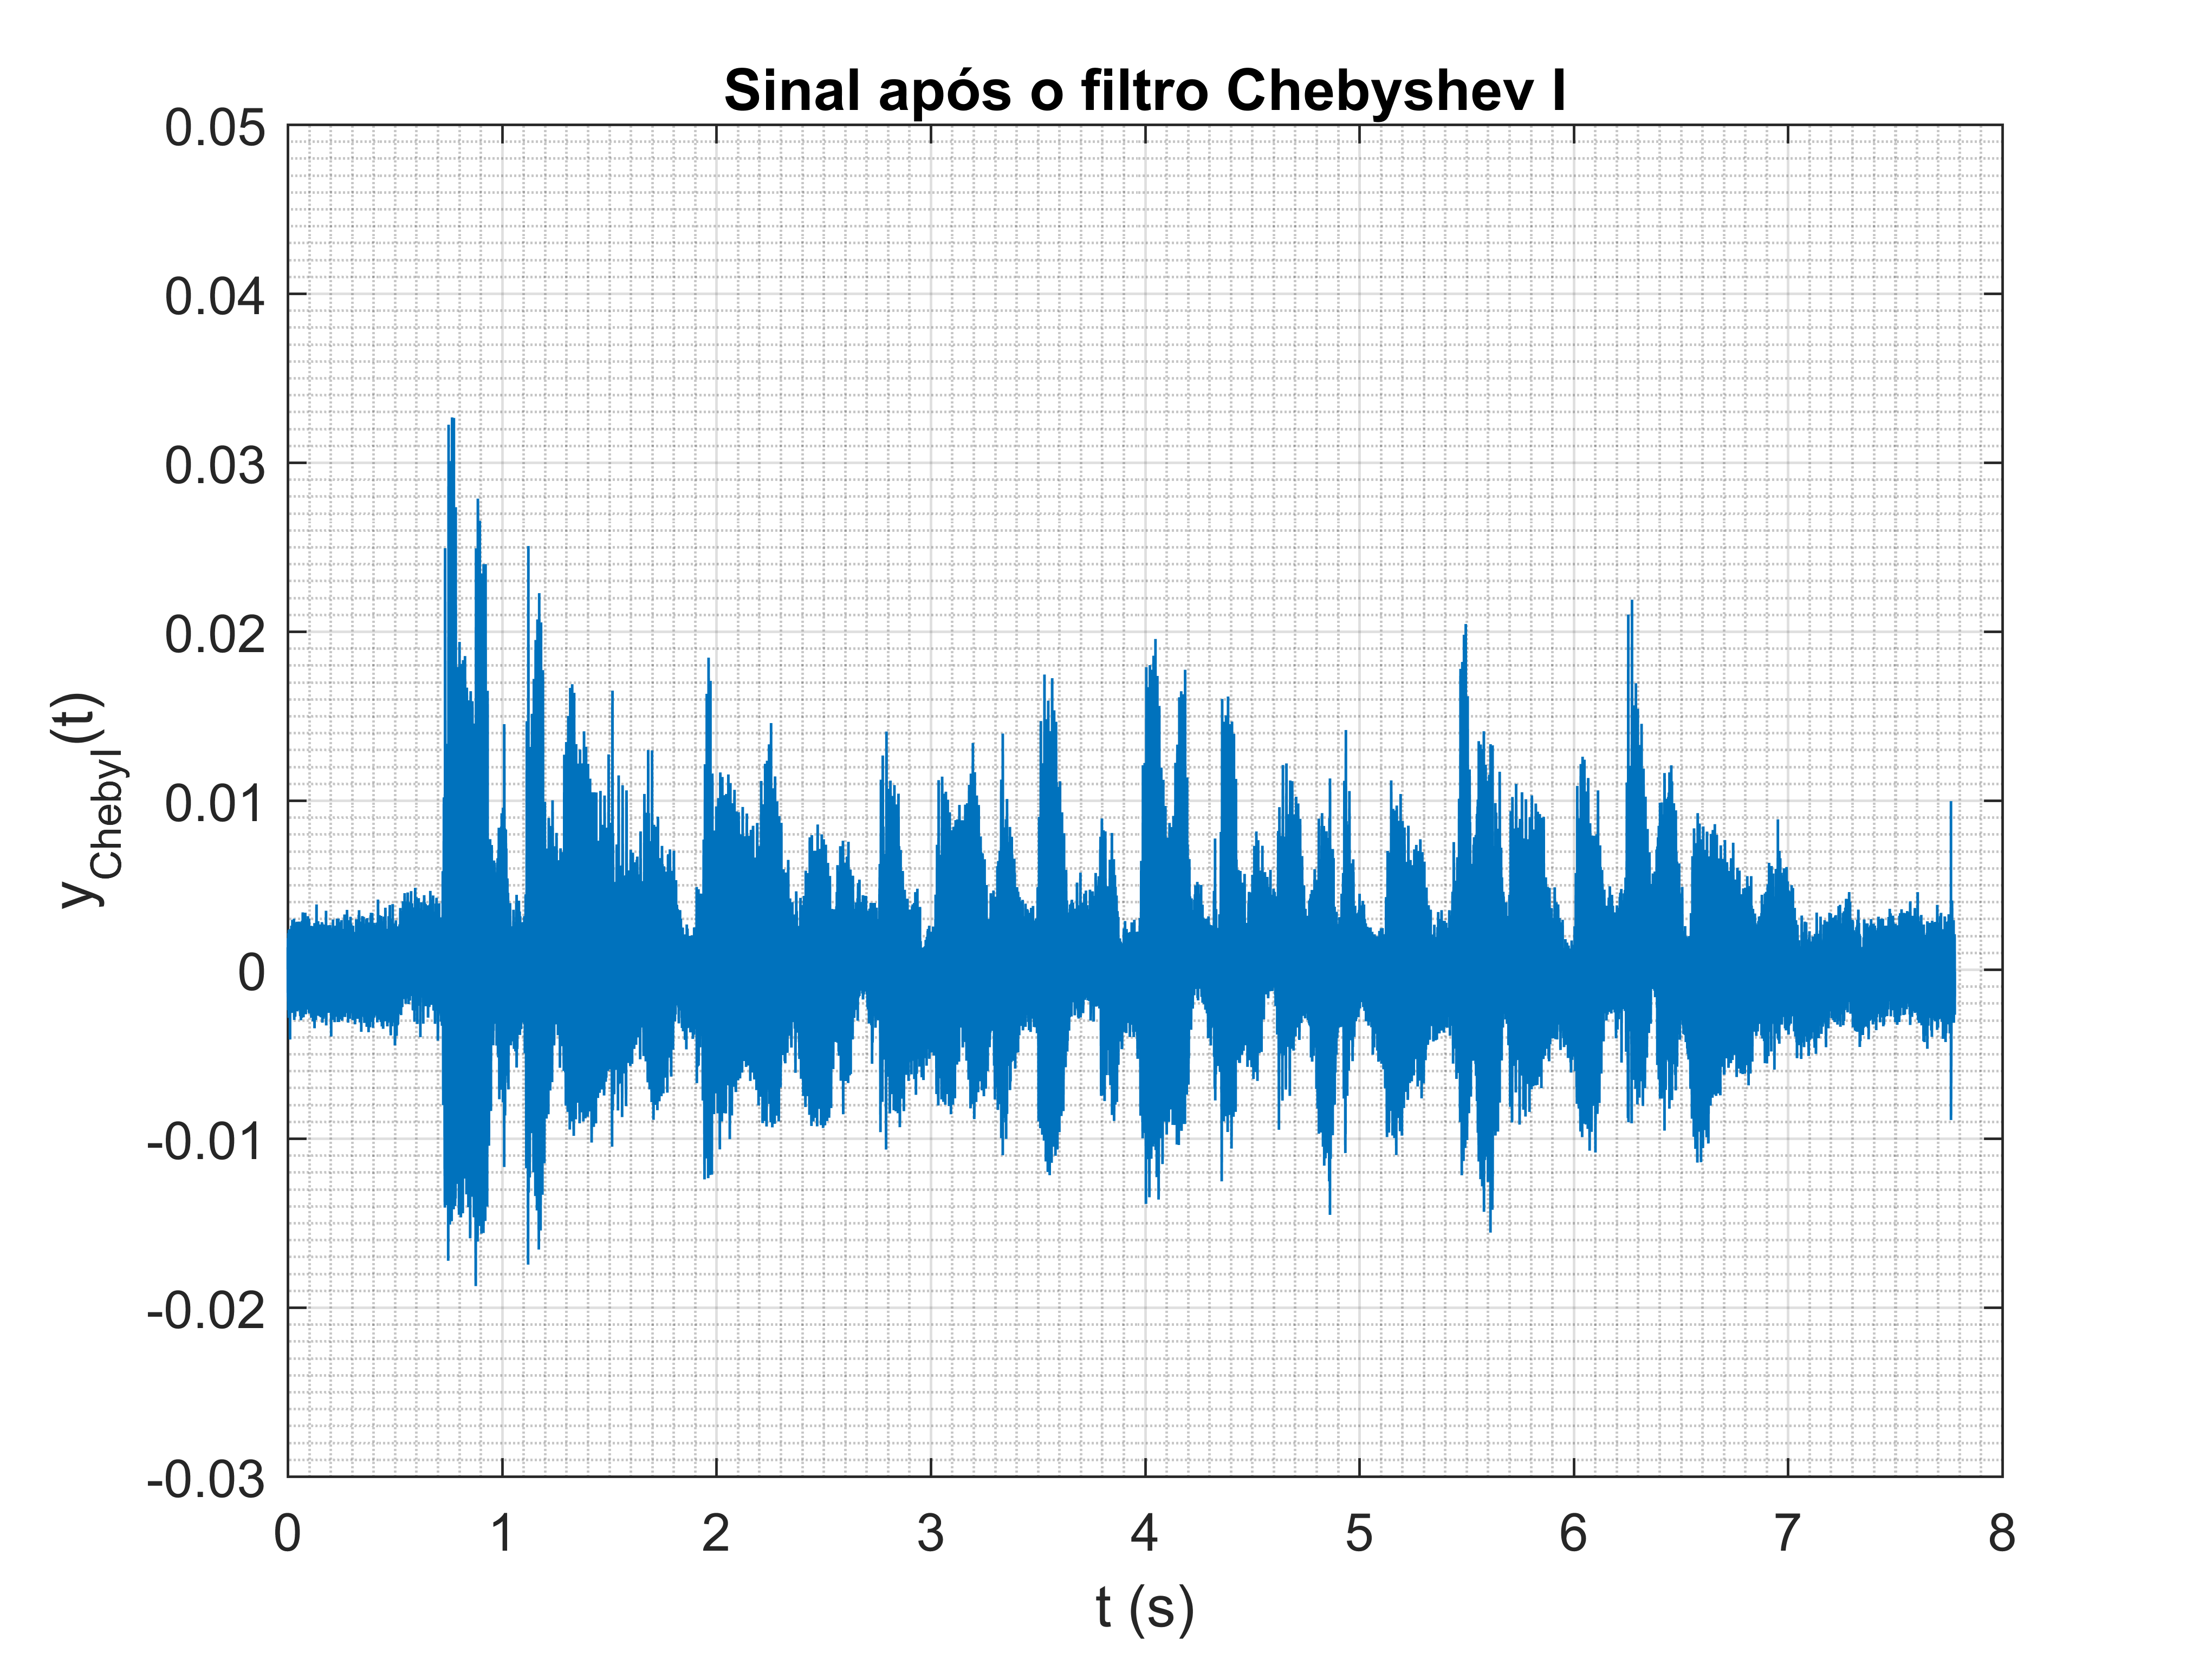
\includegraphics[width=0.7\textwidth]{graficos/filtrados_t_c1.png}
    \end{figure}
\end{frame}
\begin{frame}{Sinais no tempo - Chebyshev II}
    \begin{figure}
        \centering
        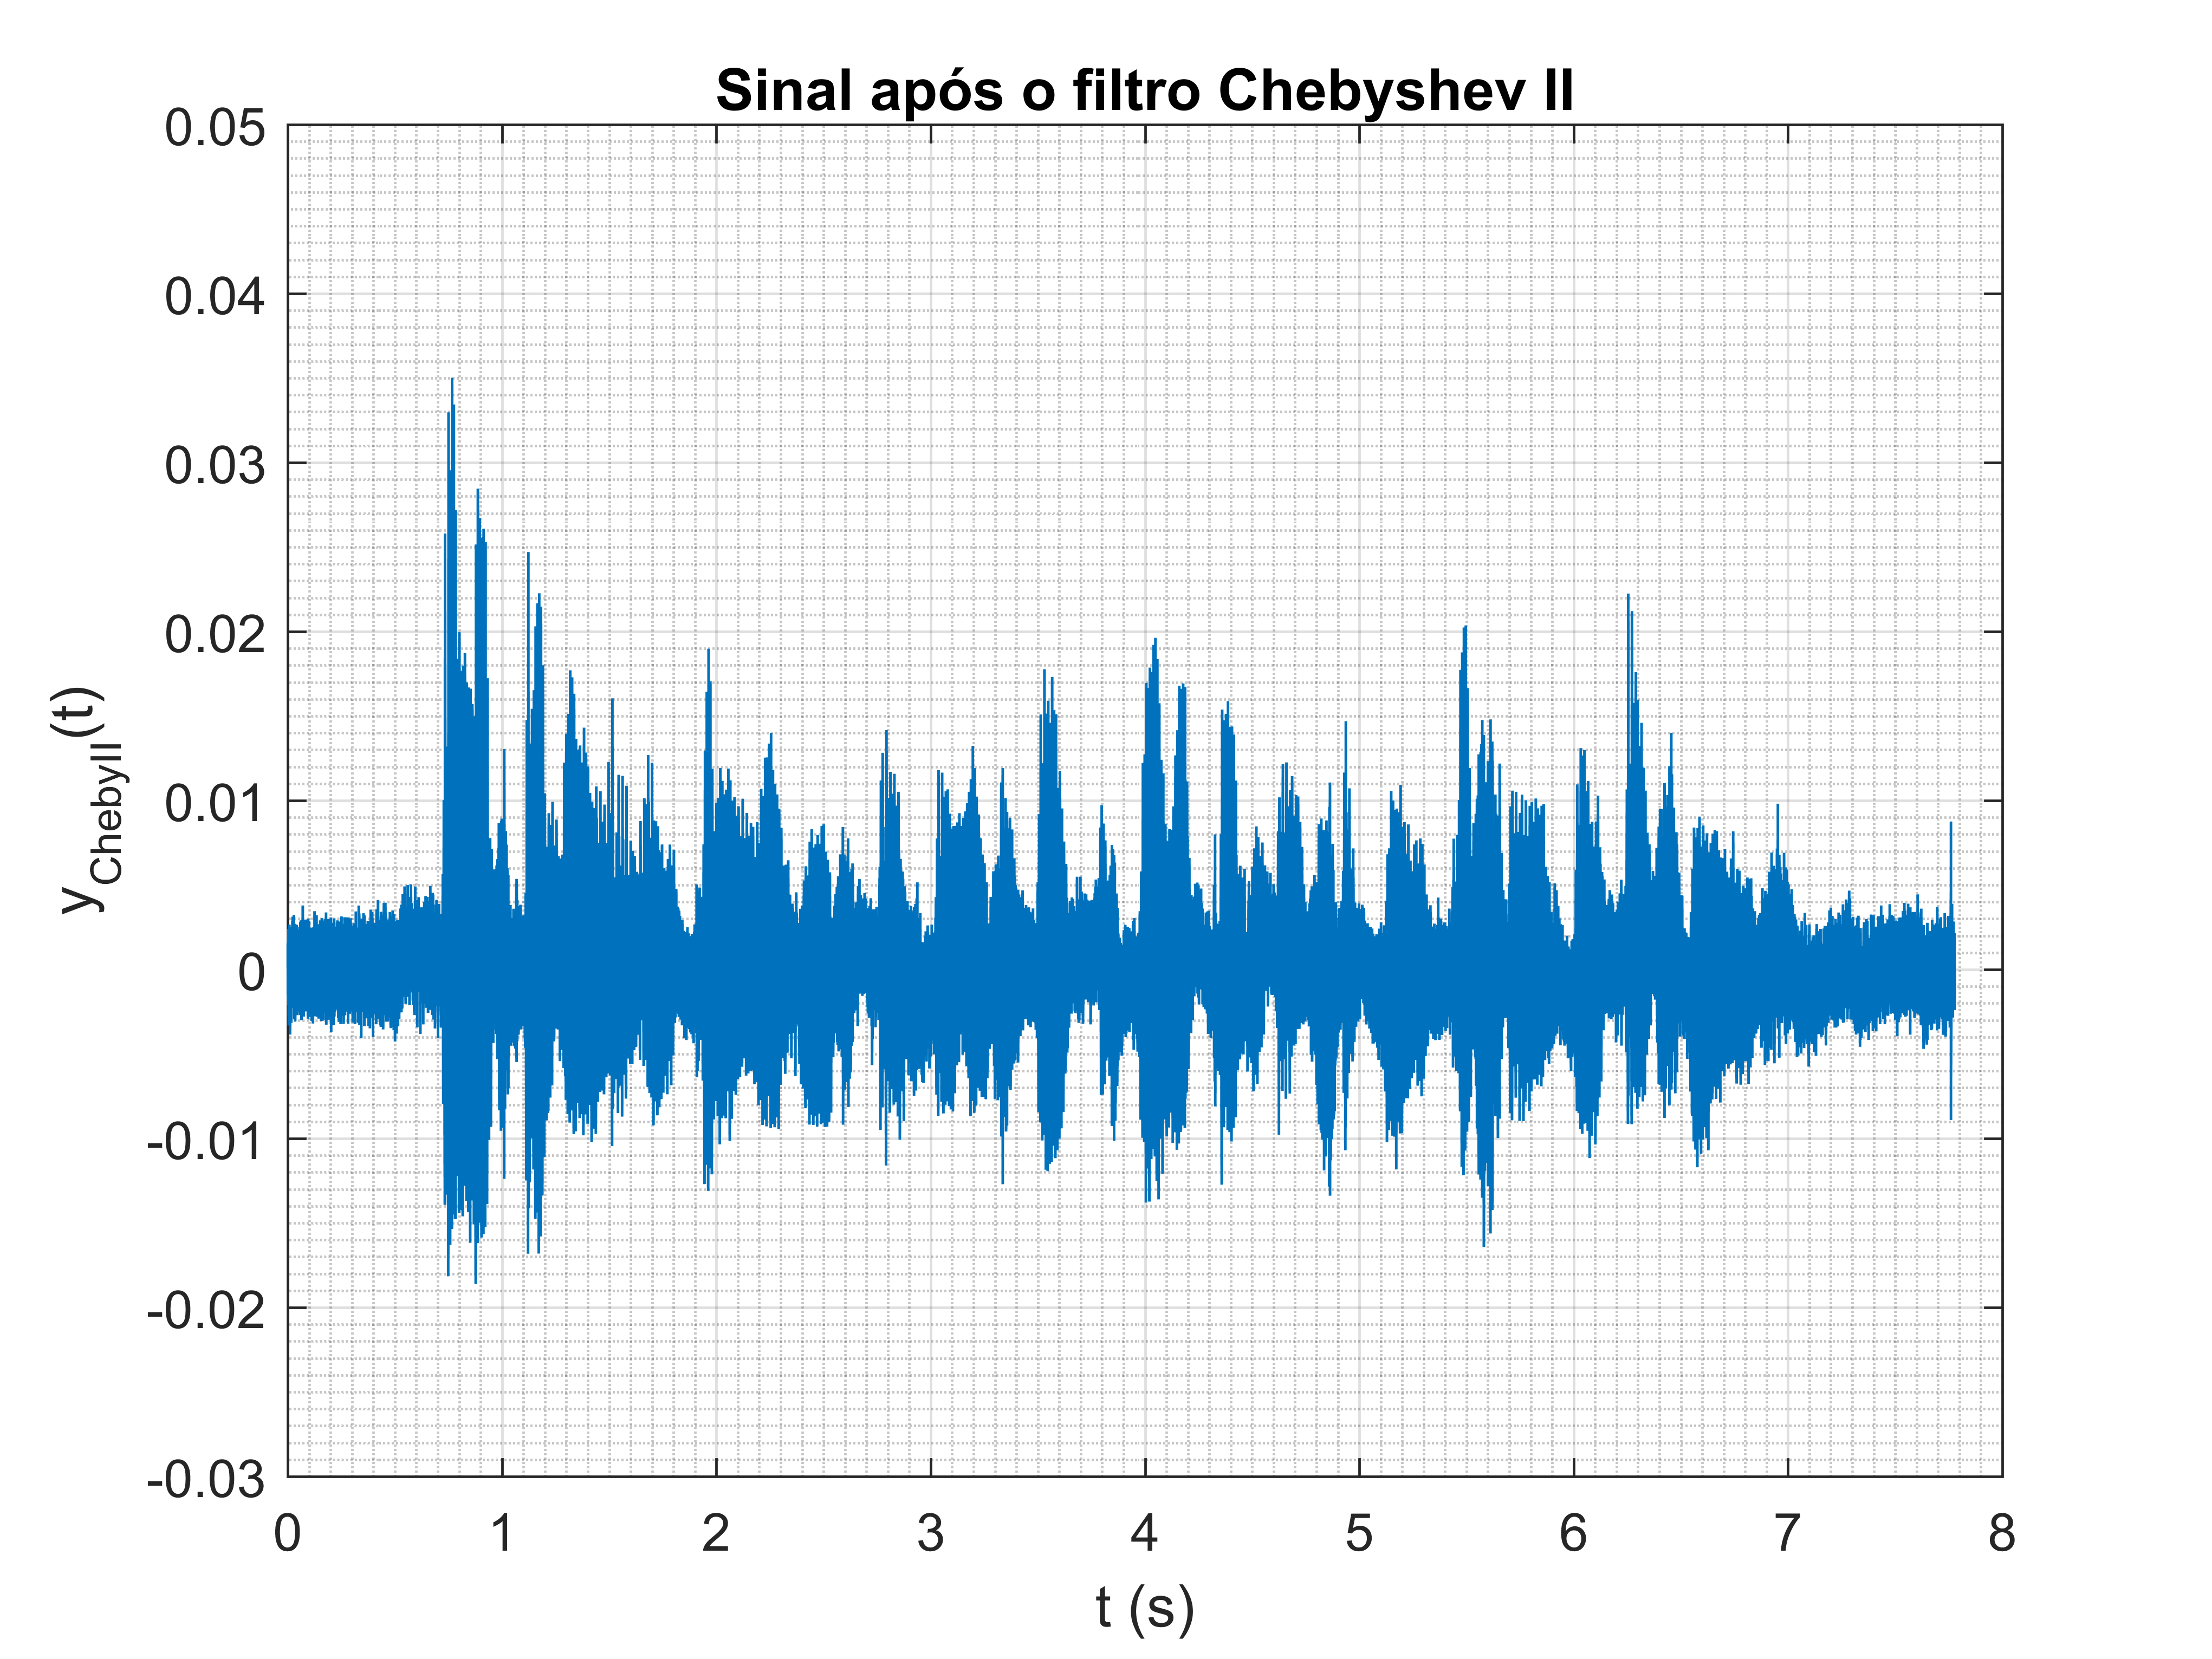
\includegraphics[width=0.7\textwidth]{graficos/filtrados_t_c2.png}
    \end{figure}
\end{frame}
\begin{frame}{Sinais no tempo - Elíptico}
    \begin{figure}
        \centering
        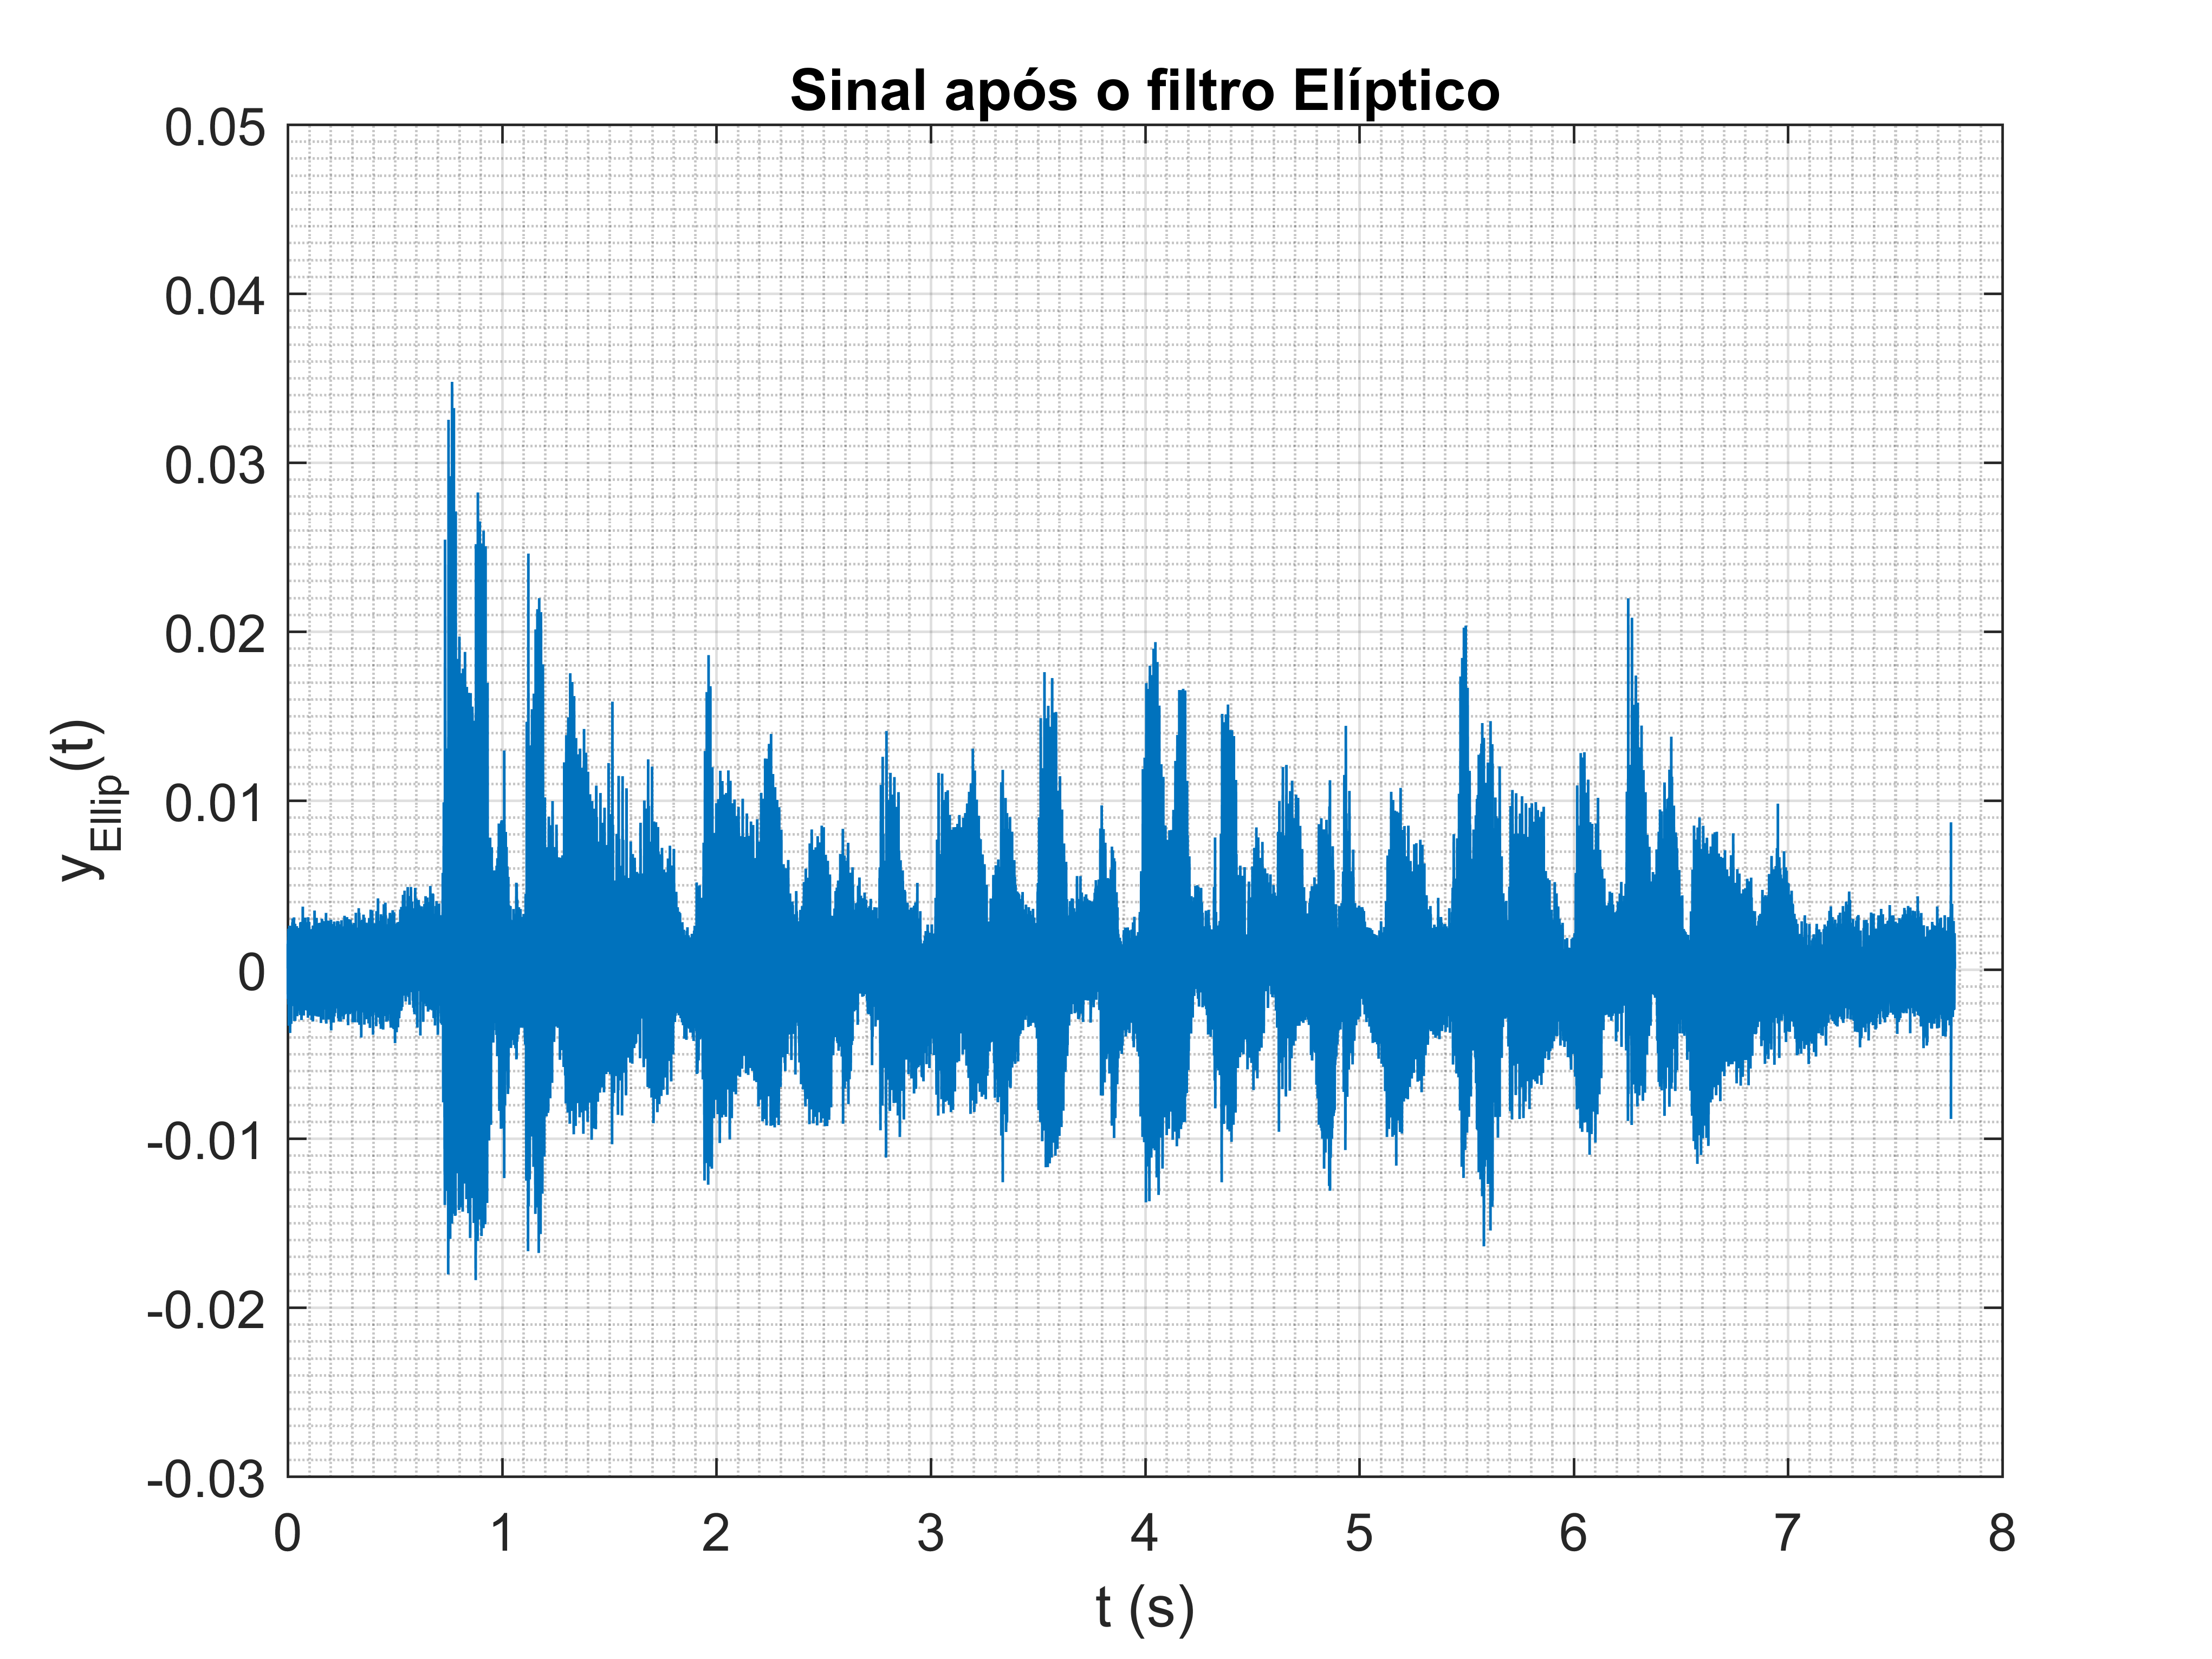
\includegraphics[width=0.7\textwidth]{graficos/filtrados_t_e.png}
    \end{figure}
\end{frame}

\begin{frame}{Sinais na frequência - Butterworth}
    \begin{figure}
        \centering
        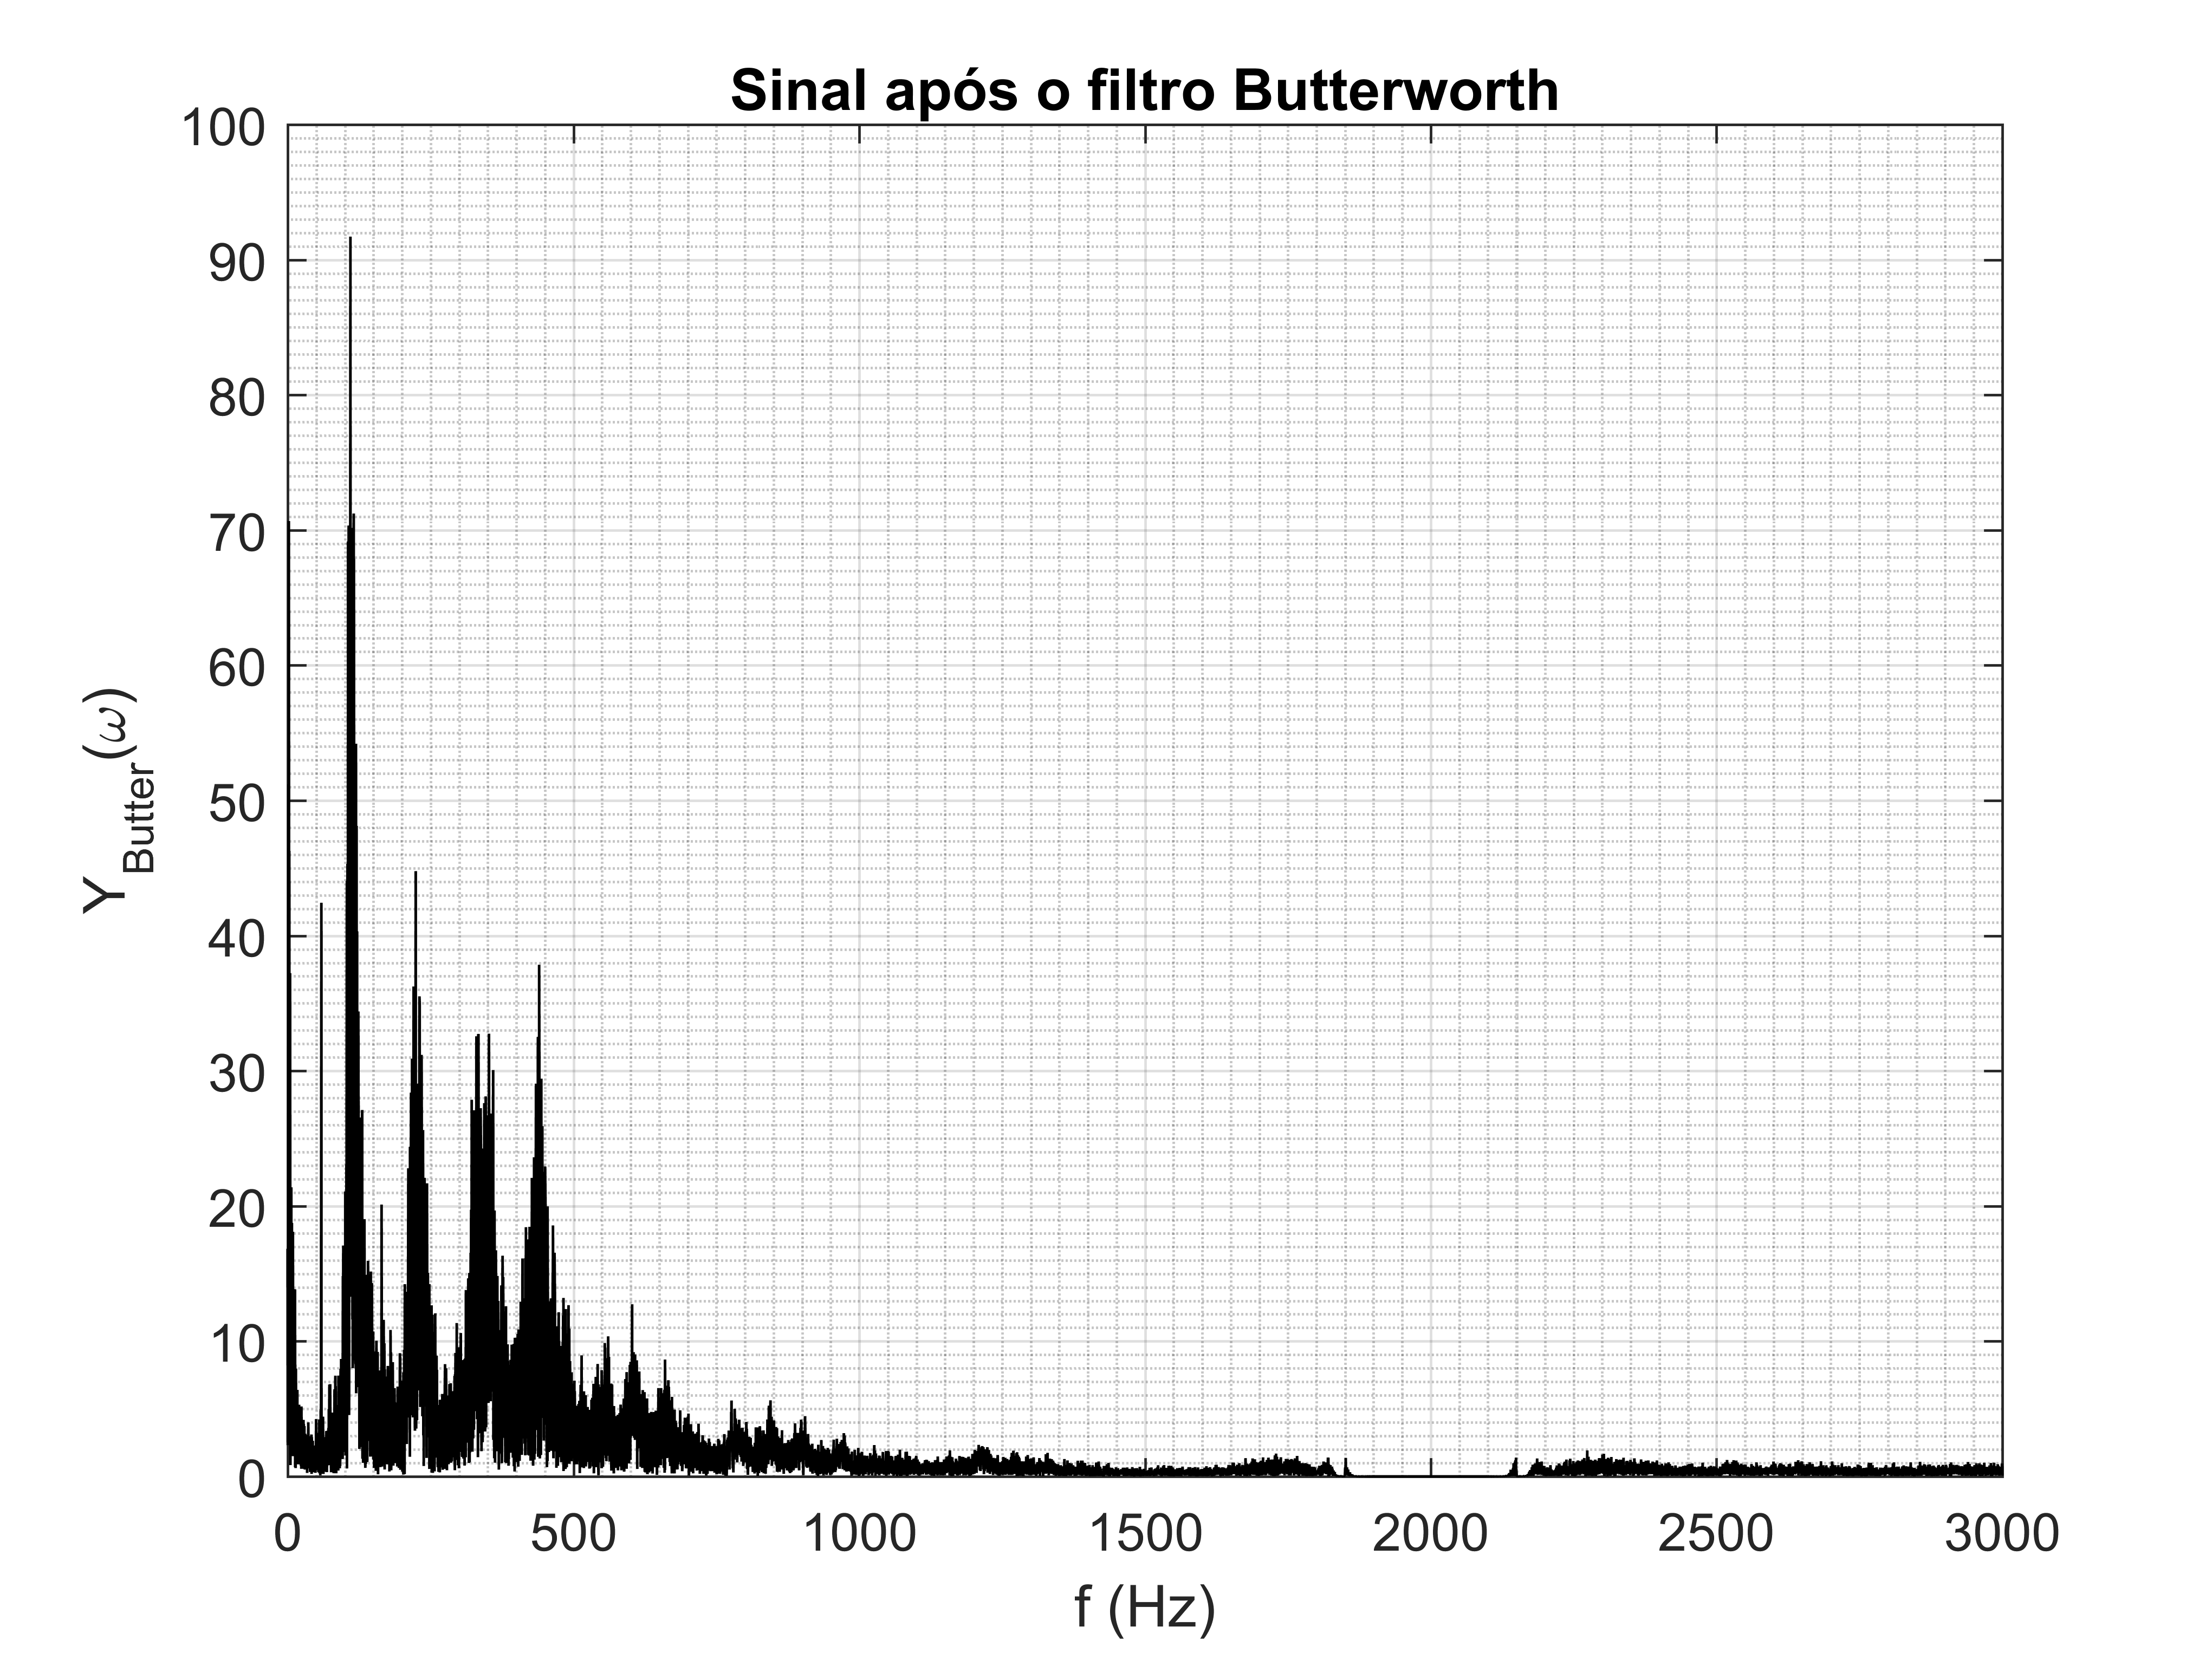
\includegraphics[width=0.7\textwidth]{graficos/filtrados_f_b.png}
    \end{figure}
\end{frame}
\begin{frame}{Sinais na frequência - Chebyshev I}
    \begin{figure}
        \centering
        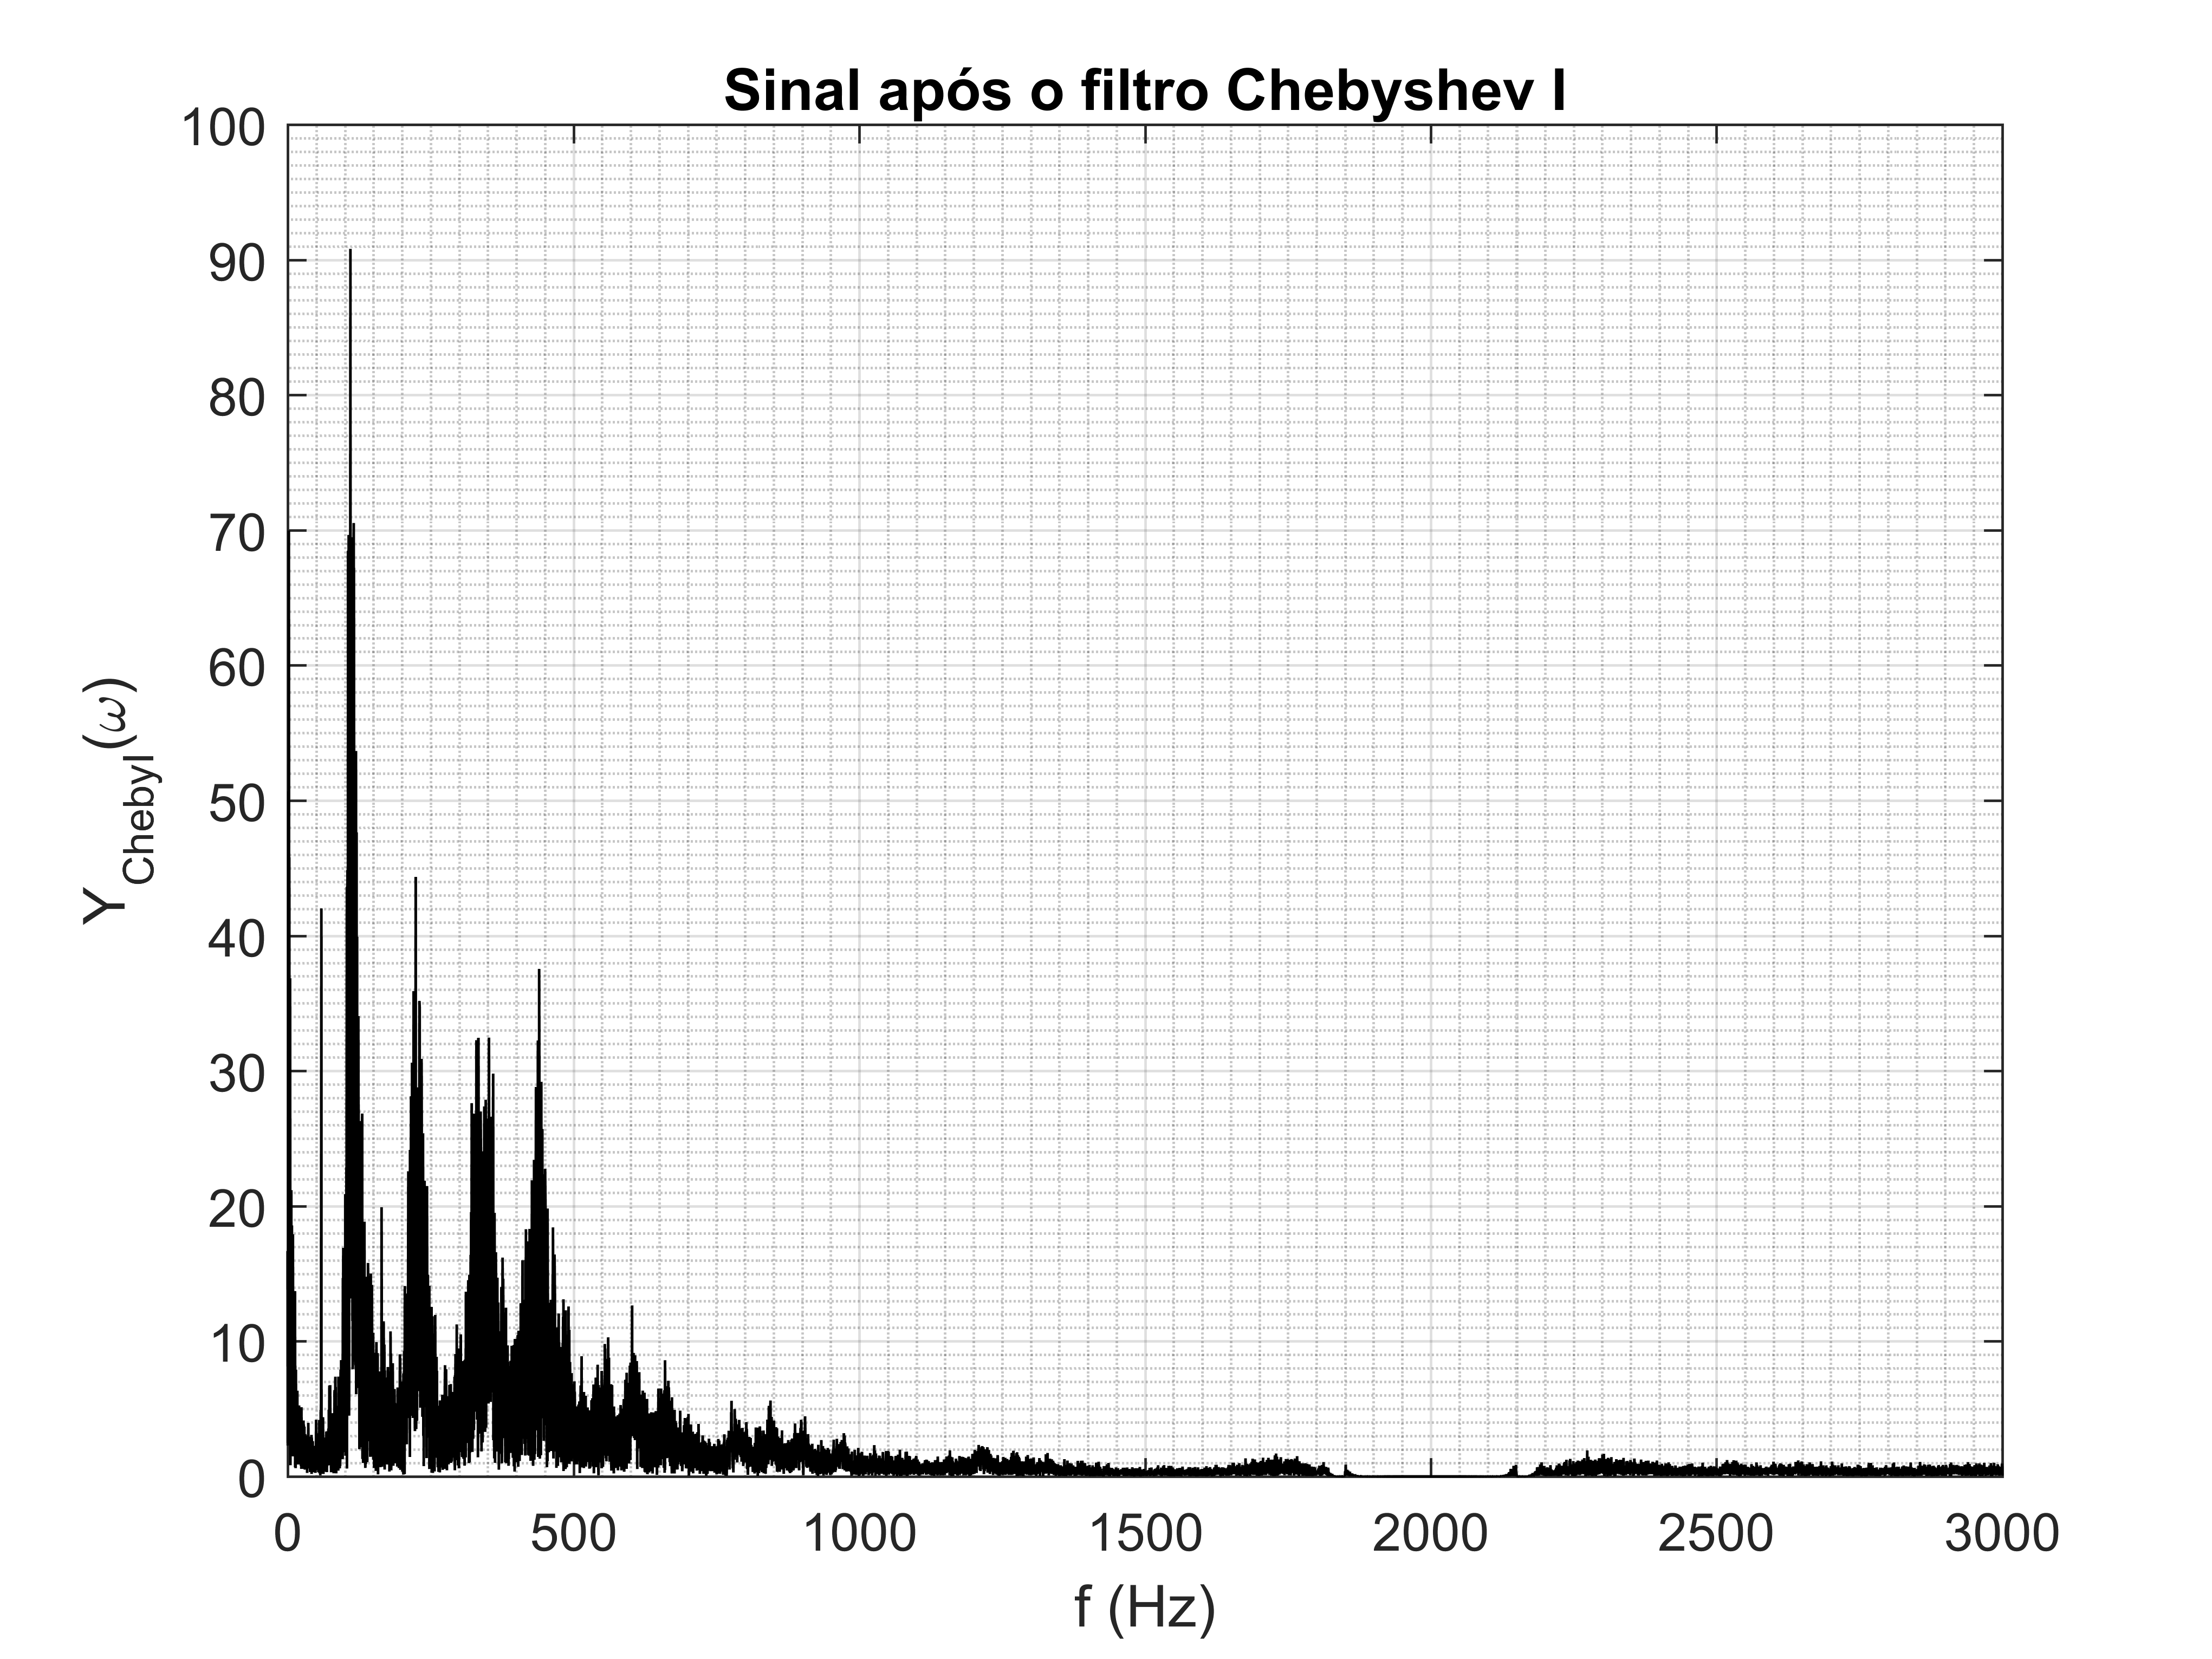
\includegraphics[width=0.7\textwidth]{graficos/filtrados_f_c1.png}
    \end{figure}
\end{frame}
\begin{frame}{Sinais na frequência - Chebyshev II}
    \begin{figure}
        \centering
        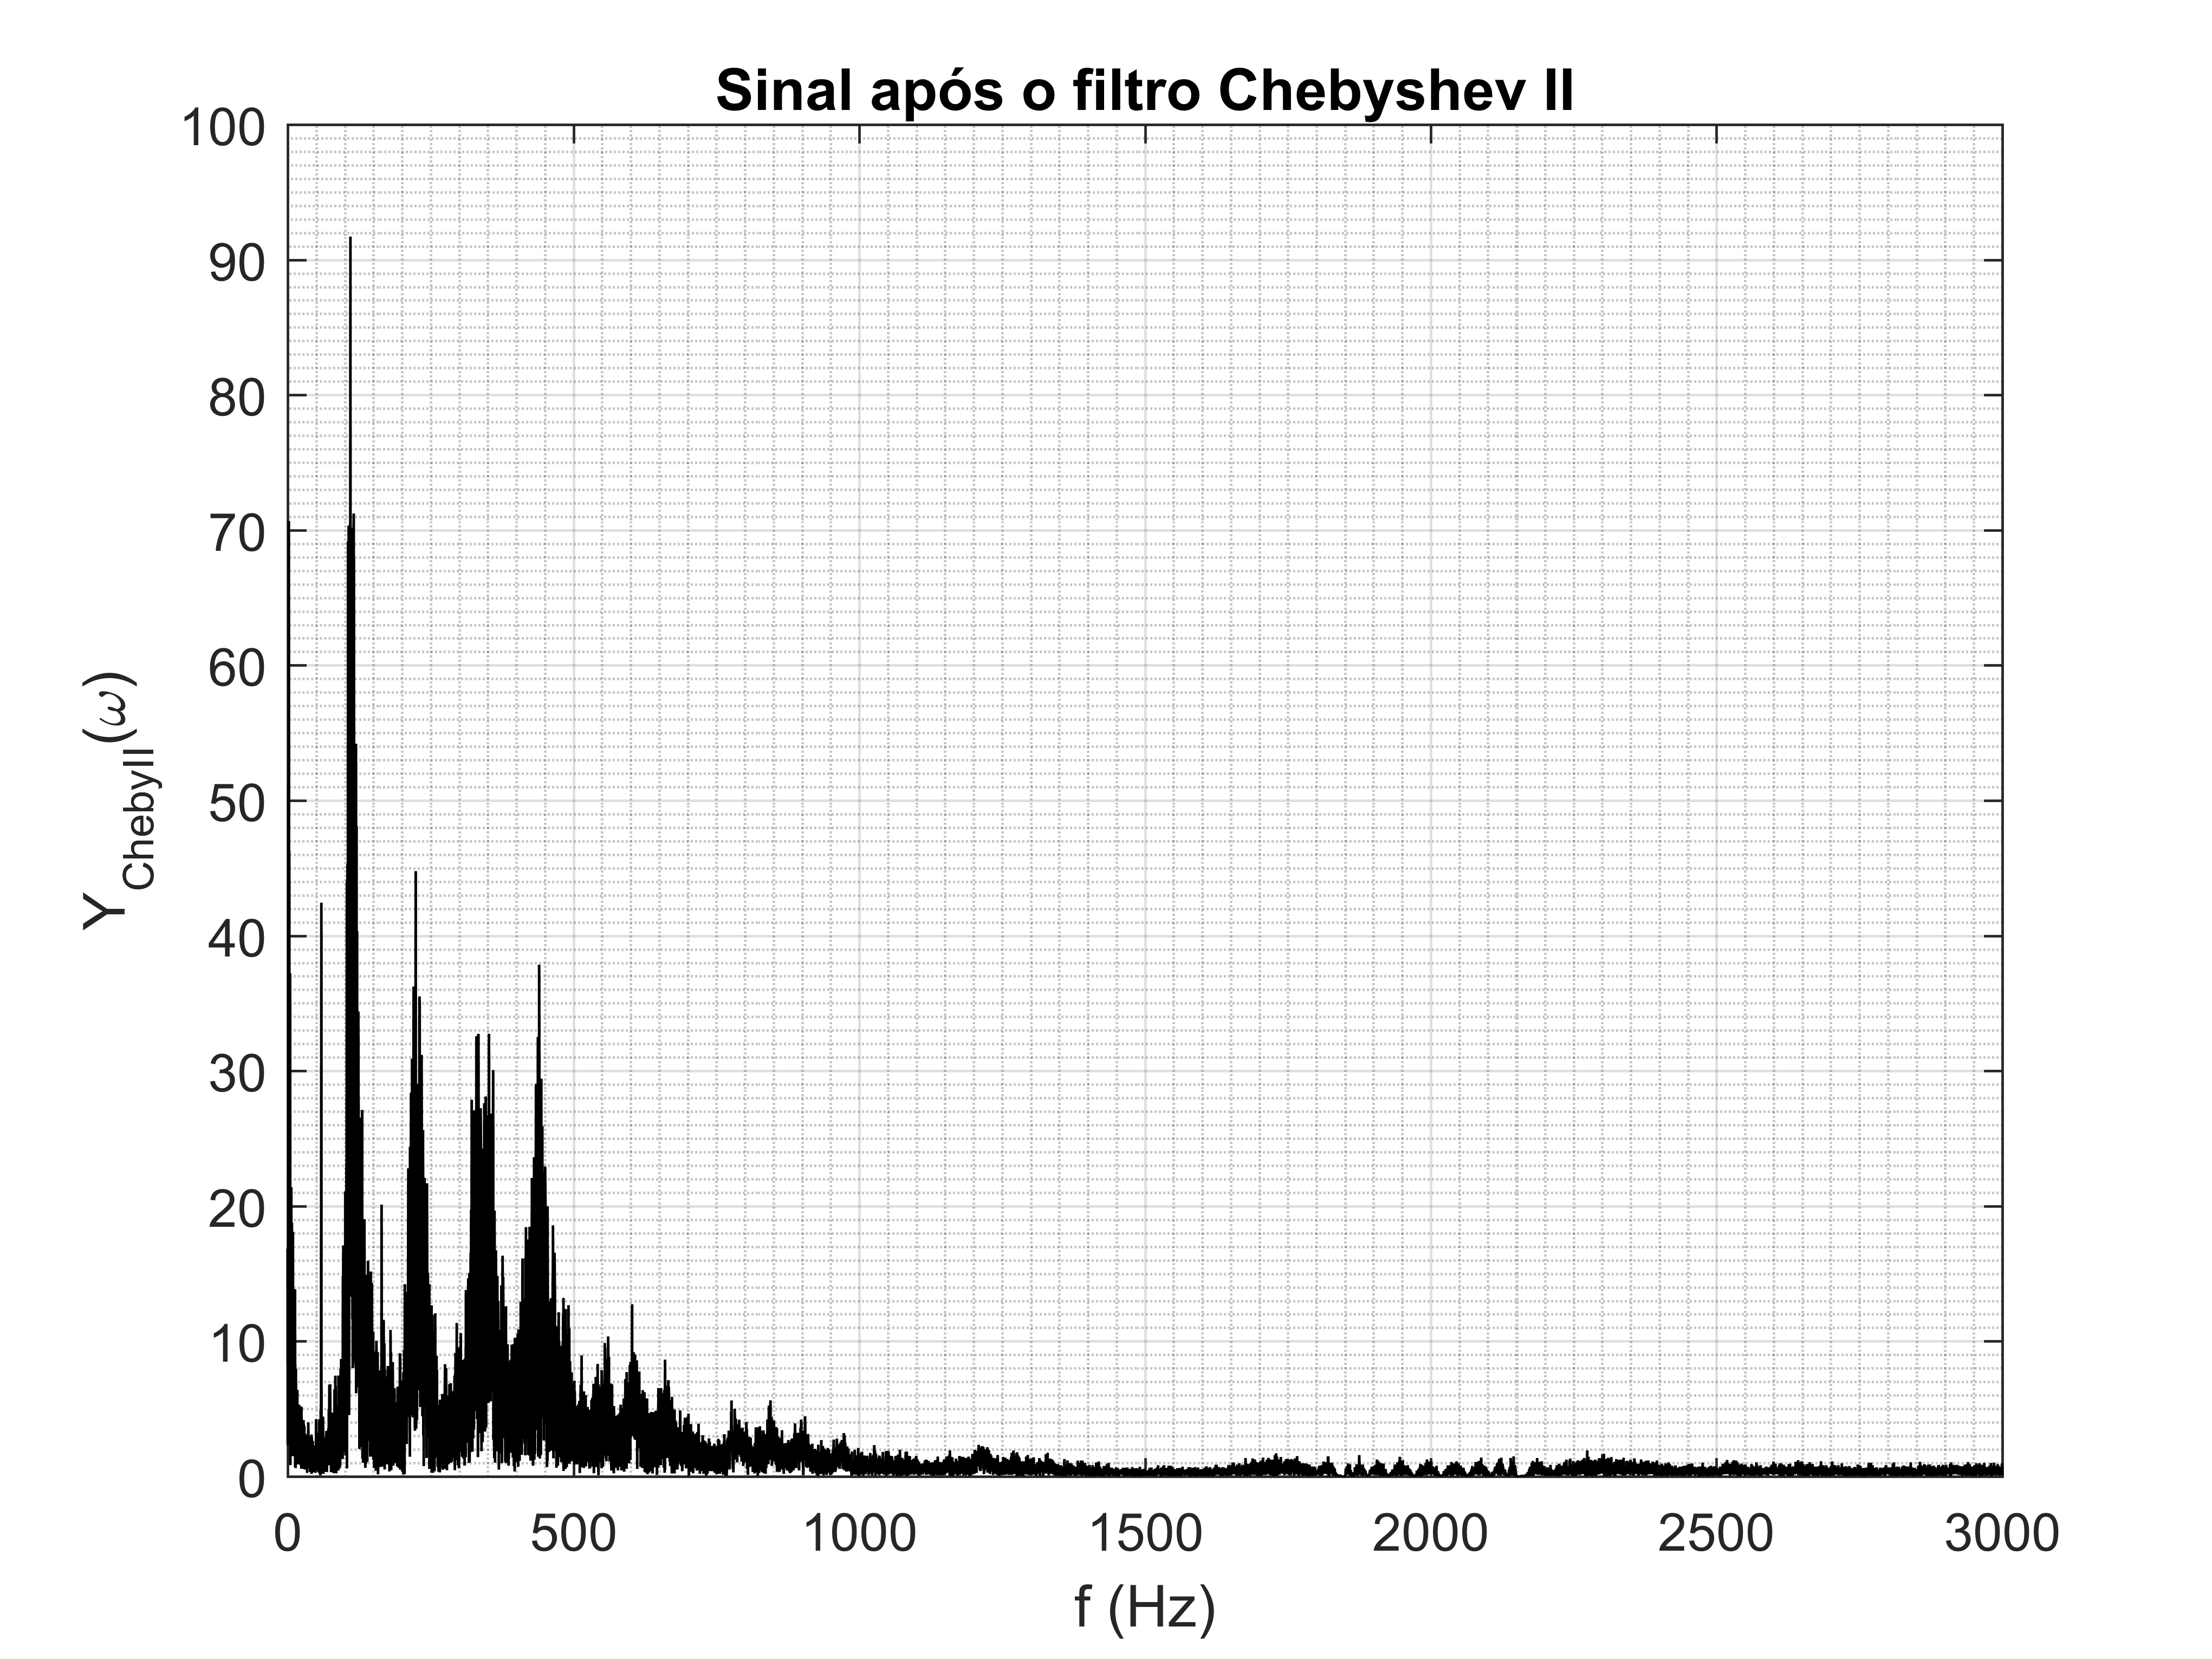
\includegraphics[width=0.7\textwidth]{graficos/filtrados_f_c2.png}
    \end{figure}
\end{frame}
\begin{frame}{Sinais na frequência - Elíptico}
    \begin{figure}
        \centering
        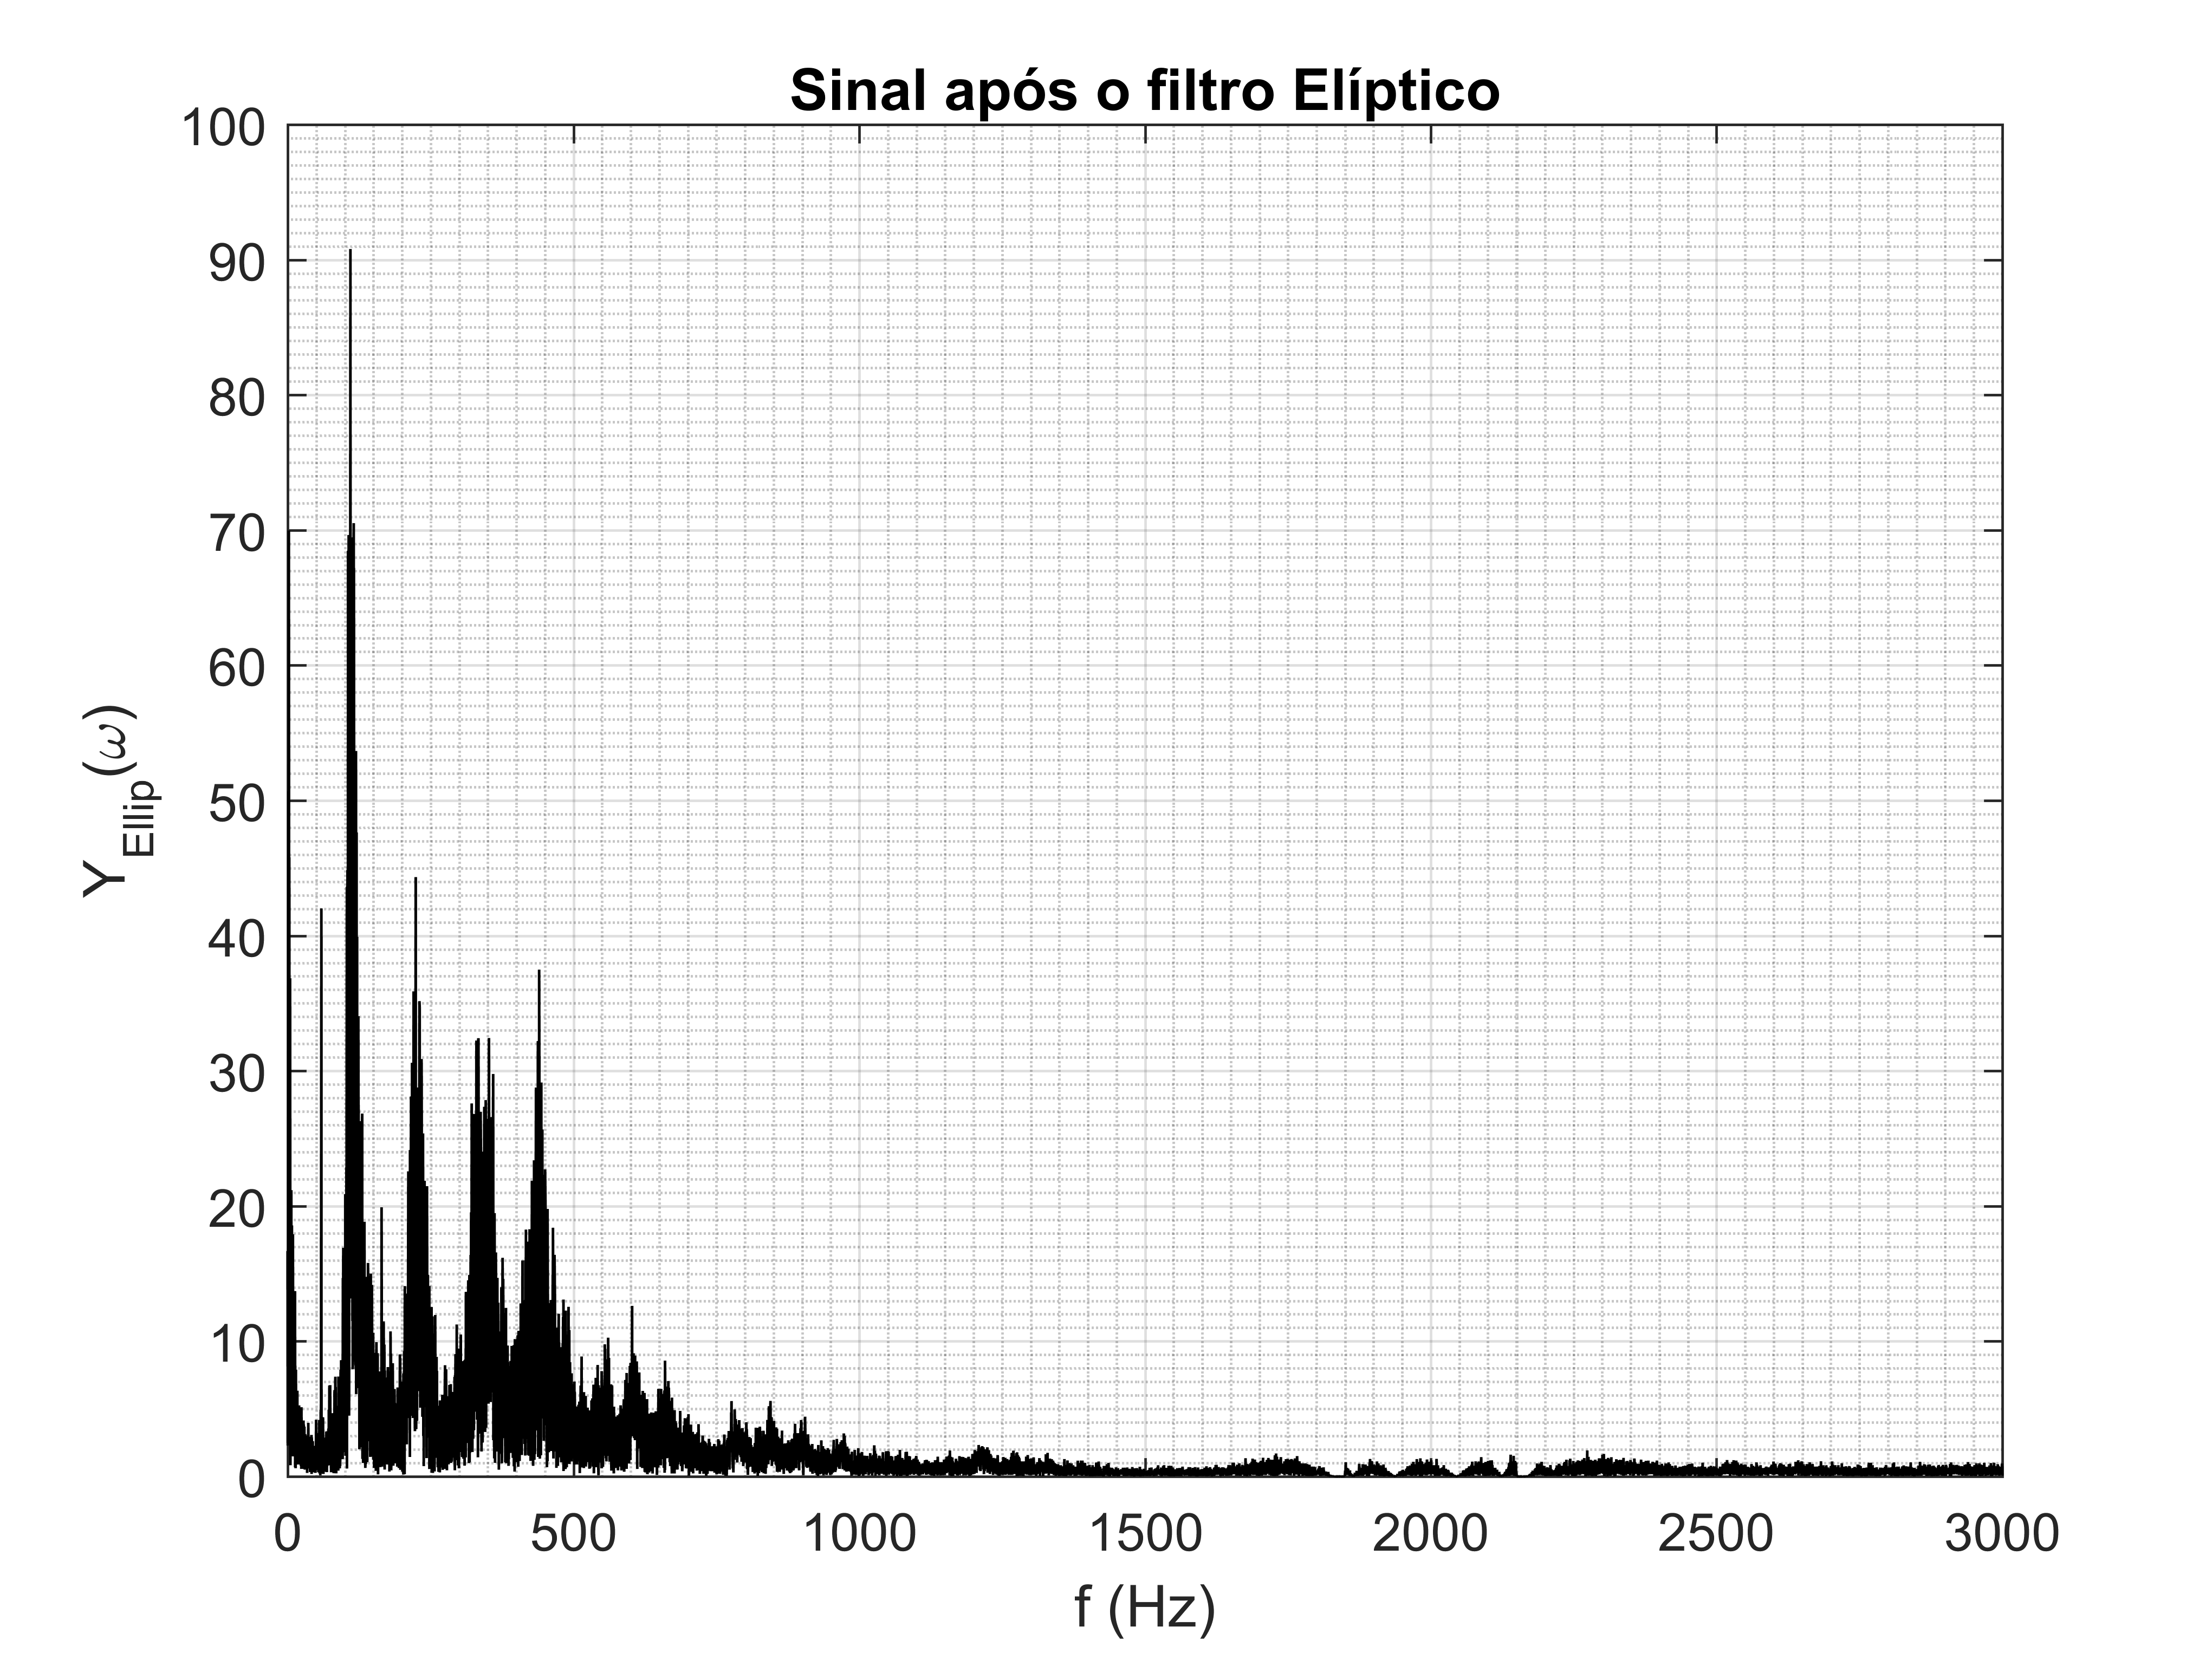
\includegraphics[width=0.7\textwidth]{graficos/filtrados_f_e.png}
    \end{figure}
\end{frame}

% Conclusao
\section{Conclusão}
\begin{frame}{Conclusão}
	\begin{itemize}
	    \item Respostas em magnitude mais próximas da ideal para um filtro foram obtidas com ordens bem menores no IIR que no FIR; 
	    \item Além das equações de projeto, a implementação de filtros IIR demanda algum conhecimento das limitações na representação numérica em computadores;
	    \item Mesmo para baixas ordens a imprecisão numérica pode mudar completamente as características de um filtros;
	    \item Representar o filtro usando seções de segunda ordem resolveu a maior parte dos problemas de imprecisão numérica;
	\end{itemize}
	
\end{frame}

% Referencias
\section{Referencias}
\begin{frame}{Referências}
	Suas referencias bibliográficas aqui, siga o modelo ABNT.
	\bibliography{bib/bibliografia}
\end{frame}

% Agradecimentos
%\section{}
%\begin{frame}{Agradecimentos}
%	Agradeço a todos. 	
%\end{frame}

\end{document}